\documentclass[a4paper,fleqn,review]{cas-sc}

\usepackage{listings}
\usepackage{latexsym}
\usepackage{amsthm}
\usepackage{longtable}
\usepackage{chemarr}
\usepackage{rotating}
\usepackage[english]{babel}
\usepackage{bm}
\usepackage{microtype}
\usepackage{csquotes}
\usepackage[authoryear,longnamesfirst]{natbib}
\bibpunct{(}{)}{;}{a}{,}{,}
\let\parencite\citep

\definecolor{celblue}{HTML}{32a2f2}
\definecolor{celgreen}{HTML}{127212}
\definecolor{ergreen}{HTML}{6eb775}
\definecolor{wsgreen}{HTML}{40FF00}
\definecolor{connred}{HTML}{ff0e0e}
\definecolor{teal}{HTML}{027979}
\definecolor{shuffleorange}{HTML}{FF5100}
\definecolor{sampledsalmon}{HTML}{ff6565}
\definecolor{connorange}{HTML}{ff9752}
\definecolor{deepblue}{HTML}{002CF1}
\definecolor{purple}{HTML}{AF7DF5}
\definecolor{lightcyan}{HTML}{8ADEF3}

\begin{document}
\let\WriteBookmarks\relax
\def\floatpagepagefraction{1}
\def\textpagefraction{.001}

\shorttitle{Hyperparameter invariance in connectome reservoirs}
\shortauthors{Churchland}

\title [mode = title]{Determinants of Hyperparameter Invariance in Connectome Reservoir Computing}

\author[1]{Miles Walter Churchland}
\credit{Conceptualization, methodology, software, formal analysis, visualization, writing - original draft, writing - review and editing}
\author[2]{Raul de Palma Aristides}
\credit{}
\author[3]{Miguel Soriano}
\credit{}
\author[4]{Anna Ritz}
\credit{}
\author[5]{Greg Anderson}
\credit{}


\affiliation[1]{organization={Department of Computer Science, Reed College},
                city={Portland},
                state={OR},
                country={United States}}

\begin{abstract}
Biological neural circuits maintain functional computation despite substantial variation in synaptic strengths, membrane properties, and inputs. Reservoir computing provides an artificial framework for studying this robustness: input signals are projected into a high-dimensional space by a fixed nonlinear dynamical system, called the reservoir. Unlike biological circuits, these systems can be highly sensitive to hyperparameters such as spectral radius, input scaling, leak rate, and bias. This paper asks which reservoir-network features support invariance to those parameter changes. Using the \textit{C.\ elegans} connectome as a biologically grounded reservoir, we measure computational capability with four task-agnostic metrics---memory capacity (MC), information processing capacity (IPC), kernel rank (KR), and generalization rank (GR)---and define hyperparameter invariance as the coefficient of variation of these metrics across sweeps of spectral radius, input scaling, leak rate, and neuron bias.

To isolate contributors to invariance, we construct controlled perturbations that separately modify connectivity topology, weight-magnitude distributions, magnitude placement, and excitatory/inhibitory sign structure while preserving the remaining properties. Across these experiments, the empirical connectome consistently occupies a relatively low-variance regime. 

The central result is a performance--invariance tradeoff: perturbations that raise task-agnostic computational capacity tend to make those capacities more dependent on reservoir hyperparameters. The controls rule out a simple explanation based on any single network feature. In the reservoir abstraction studied here, global excitatory/inhibitory sign imbalance is an important control parameter, but its effect is conditional on the topology on which signs are placed and on the distribution and placement of weight magnitudes. Thus, the biological sign structure is not interpreted as an optimum for reservoir performance; instead, it participates in a broader structural regime that favors lower hyperparameter sensitivity. These findings suggest that robust reservoir computation arises from coordinated constraints on sign balance, topology, and synaptic-weight organization, rather than from a universally primary determinant.
\end{abstract}

\begin{highlights}
\item The \textit{C.\ elegans} connectome occupies a low hyperparameter-sensitivity regime as a reservoir.
\item Higher task-agnostic capacity often coincides with higher sensitivity to reservoir hyperparameters.
\item E/I sign imbalance is a strong but conditional control, interacting with topology and weight placement.
\end{highlights}

\begin{keywords}
reservoir computing \sep connectomics \sep hyperparameter robustness \sep E/I balance \sep \textit{C.\ elegans}
\end{keywords}

\maketitle

\section{Introduction}
Reservoir computing uses a fixed recurrent dynamical system to project input histories into a high-dimensional state space, after which only a readout is trained \parencite{jaeger_echo_state_2001,maass_lsm_2002}. This separation makes reservoir models useful for studying how recurrent architecture shapes computation. It also exposes a persistent design problem: reservoir behavior can depend strongly on hyperparameters such as spectral radius, input scaling, leak rate, and neuronal bias. A reservoir that performs well only under a narrow set of choices is less useful as a robust computational substrate.

Most reservoir-computing theory and practice treats random recurrent networks as a strong generic baseline. Random reservoirs can provide diverse, weakly correlated nonlinear features and can be tuned near dynamical regimes that support memory and separability \parencite{Lukosevicius2012PracticalESN}. From that perspective, a small, sparse, structured, signed biological circuit should not be expected to maximize generic task-agnostic capacity. The \textit{C.\ elegans} connectome was shaped by developmental, metabolic, behavioral, and stability constraints, not by the objective of serving as an optimized random feature map. Its value here is therefore not as a presumed best reservoir, but as a structured biological prior for asking which constraints change the relationship between performance and sensitivity.

This distinction matters because biological neural systems often remain functional across variable internal and environmental conditions, whereas artificial systems can be brittle outside the regime in which they were tuned or trained \parencite{recht2019,geirhos_jacobsen_michaelis_zemel_brendel_bethge_wichmann_2020}. In reservoir computing terms, this suggests a question that is different from peak-performance optimization: which structural properties make computational statistics stable across hyperparameter variation? The present study addresses that question by treating hyperparameter invariance as a metric of reservoir architectures.

We use the signed chemical-synapse \textit{C.\ elegans} connectome as a biologically grounded reservoir and compare it with controlled perturbations that isolate topology, excitatory/inhibitory sign structure, weight-magnitude distribution, magnitude placement, and sign placement. Reservoir behavior is evaluated with four task-agnostic metrics: memory capacity (MC), information processing capacity (IPC), kernel rank (KR), and generalization rank (GR). Hyperparameter invariance is quantified as the coefficient of variation of these metrics across a full factorial sweep of spectral radius, input scaling, leak rate, and neuron-bias range.

The results identify a performance--invariance tradeoff rather than a biological optimum for reservoir performance. Perturbations that increase task-agnostic capacity often also increase sensitivity to hyperparameter choice. Global excitatory/inhibitory sign imbalance strongly influences low-variance regime observed in the \textit{C.\ elegans} model studied here, but it is not a universal determinant acting alone: its effect depends on topology, local sign placement, weight-magnitude distribution, and magnitude placement. 

\section{Methods}
\label{sec:methods}
\subsection{Reservoir model}
We use echo state networks, a discrete-time reservoir-computing model in which recurrent weights are fixed and only linear readouts are fit when a metric requires reconstruction \parencite{jaeger_echo_state_2001,Lukosevicius2012PracticalESN}. Let \(u_t \in \mathbb{R}^{d}\) be the input, \(x_t \in \mathbb{R}^{N}\) the reservoir state, and \(y_t \in \mathbb{R}^{p}\) the readout. With leak rate \(\alpha \in (0,1]\), the state update is
\begin{align}
\tilde{x}_{t+1} &= \tanh\!\left(W^{\mathrm{res}} x_t + s_{\mathrm{in}}W^{\mathrm{in}} u_{t+1} + b + \xi_t\right), \\
x_{t+1} &= (1-\alpha)\,x_t + \alpha\,\tilde{x}_{t+1}, \\
y_t &= W^{\mathrm{out}}\,x_t.
\end{align}
Here \(W^{\mathrm{res}}\in\mathbb{R}^{N\times N}\) is the sparse recurrent reservoir matrix, \(W^{\mathrm{in}}\) is the input matrix, \(s_{\mathrm{in}}\) scales the input drive, \(b\in\mathbb{R}^{N}\) is a fixed per-neuron bias vector, and \(\xi_t\) denotes optional noise. Noise is not included in the experiments. The readout dimension is \(p=3\) for IPC so that multiple polynomial orders can be solved in a single batch; otherwise \(p=1\).

Only \(W^{\mathrm{out}}\) is fit during metric calculations. The recurrent matrix is fixed after the architecture is instantiated, so the experiments isolate how reservoir structure and global hyperparameters shape the state matrix available to the readout. Architectures are rescaled to a target spectral radius before rollout, as described below. This keeps the comparison focused on relative structure rather than raw matrix scale.

\subsection{Reservoir hyperparameters}
The experiments sweep four hyperparameters that control the reservoir's operating regime. The spectral radius \(\rho(W^{\mathrm{res}})\) controls the strength of recurrent feedback, where
\[
\rho(W) = \max_{1 \le i \le N} |\lambda_i|.
\]
The leak rate \(\alpha\) controls the effective timescale of the reservoir by interpolating between the previous state and the newly computed activation. Input scaling \(s_{\mathrm{in}}\) controls the strength of the external drive relative to recurrent feedback. The neuron-bias half-range \(\beta\) controls static activation offsets: when \(\beta=0\), \(b=0\); when \(\beta>0\), each neuron is sampled independently as \(b_i\sim\mathcal{U}(-\beta,\beta)\) and then held fixed during trials. These parameters do not alter the trained readout directly; they change the dynamics of the reservoir whose stability is evaluated by the invariance analysis.
\subsection{Connectome data and preprocessing}
\label{sec:connectome_dataset}
A connectome is a description of the neural wiring of an organism. It encodes which neurons are connected, the direction of each connection, and often additional biological metadata such as the number of synaptic terminals and the neurotransmitter associated with each connection.

In this work, we treat the connectome as the foundation for a graph: each neuron is represented as a node, and each synapse as a directed, weighted edge. Two \textit{C.\ elegans} connectome sources are used. The main experiments use the signed chemical-synapse connectome derived from EleganSign \parencite{fenyves_szilágyi_zsolt_vassy_csaba_2020,elegansign_web}. We analyze two preprocessing versions of this dataset. In the signed-only version, unknown or complex-sign connections are removed, leaving 297 nodes and 1740 directed signed edges. In the augmented random-sign version, the 1864 unknown or complex-sign edges are retained and assigned signs randomly with a 4:1 excitatory-to-inhibitory ratio. The older c302-derived connectome \parencite{c302} is retained only for the supplemental architecture visualizations and legacy schematic controls; it is not the source of the main results figures.

The signed-only graph contains 1740 directed chemical-synapse edges over 297 neurons after preprocessing. These signs are treated as the empirical excitatory/inhibitory partition for the invariance experiments. The augmented random-sign graph adds the 1864 unknown or complex-sign connections back into the topology and assigns each such edge a random sign under a 4:1 excitatory-to-inhibitory prior. This assignment is used as a sensitivity analysis rather than as a claim that those individual signs are known. Both versions remain \emph{working abstractions}: they do not attempt to capture receptor-specific, context-dependent, developmental, or neuromodulatory effects. Because this study examines how coarse sign structure and weight statistics influence task-agnostic reservoir metrics across hyperparameter sweeps, incorporating detailed synapse-type dynamics is beyond the scope of the analysis and computationally expensive at the current scope of our experiments.

When edge magnitudes are required, the number of synaptic contacts from neuron \(i\) to neuron \(j\) is used as a weight proxy, \(W_{ij}=c_{ij}\). Treating contact number as a proxy weight is standard in \emph{C.\ elegans} modeling \parencite{c302,Casal2020,churchland_garcia-ojalvo_2026} and provides the biologically informed magnitude prior for the reservoir.

\subsubsection{Omitted and isolated nodes}
\label{sec:omission}
The final analysis graph contains 297 nodes after preprocessing. Nodes or entries with no neuronal in- or out-edges are dynamically inert in this reservoir model and therefore do not influence the dynamics of the connected network. Formally, if neuron \(i\) satisfies \(W_{ij}=0\) and \(W_{ji}=0\) for all \(j\), then its state does not contribute to the state update of any other neuron. Consequently, adding or removing such isolated nodes does not alter the dynamics of the remaining recurrent network. They may still receive an input-driven internal signal, but that signal provides no graph-mediated recurrent features to the readout layer. The omission of isolated or non-neuronal entries is therefore a preprocessing step rather than a biological claim about their importance in the animal.
\subsection{Task-agnostic reservoir metrics}
Task-agnostic reservoir statistics measure computational properties of the reservoir before training it on a specific downstream task. This study uses four such metrics: kernel rank (KR), generalization rank (GR), memory capacity (MC), and information processing capacity (IPC), following prior work on reservoir/neural-microcircuit diagnostics and benchmarking \parencite{maass_comp_power_2004,Jaeger2002STMESN,dambre_ipc_2012,pilati_ceni_michieletti_gallicchio_ricciardi_milano_2026}. For each architecture and hyperparameter setting, the reservoir is driven by an i.i.d. input sequence and the resulting state matrix is used to compute these metrics. Higher MC, IPC, and KR indicate greater task-agnostic computational capability. GR measures sensitivity to small input perturbations; throughout the results it is analyzed alongside the other metrics as a reservoir response statistic.

\subsubsection{Kernel Rank}
Kernel rank measures how many effectively independent reservoir activity dimensions are produced by the input drive \parencite{maass_comp_power_2004}. We collect the post-washout state matrix \(X\in\mathbb{R}^{T\times N}\), center it over time, compute singular values \(S=\{\sigma_i\}\), normalize them as \(p_i=\sigma_i/\sum_j\sigma_j\), and compute effective rank:
\[
\mathrm{KR}
=
\exp\left(-\sum_i p_i\ln p_i\right).
\]
This effective-rank formulation captures the spread of activity across orthogonal modes rather than exact linear independence alone \parencite{roy_effective_rank_2007}.

\subsubsection{Generalization Rank}
Generalization rank measures how reservoir states change under small input perturbations \parencite{maass_comp_power_2004}. Let \(u_t\sim\mathcal{U}(-1,1)\) be the clean input and \(u'_t=u_t+\kappa\varepsilon_t\), where \(\varepsilon_t\sim\mathcal{N}(0,1)\) and \(\kappa=0.01\). If \(X\) and \(X'\) are the corresponding post-washout state matrices, then
\[
\mathrm{GR}
=
\mathrm{erank}(X'-X).
\]

\subsubsection{Memory Capacity}
Memory capacity measures how well a linear readout can reconstruct past inputs from the current reservoir state \parencite{Jaeger2002STMESN}. For each delay \(d\), a ridge-regression readout is trained to predict \(u(t-d)\) from \(x(t)\), and the squared Pearson correlation between predicted and true delayed input is recorded. We approximate total memory capacity by summing over delays:
\[
\mathrm{MC}
=
\sum_{d=1}^{D_{\max}}
r_{\mathrm{score}}(u(t-d),\hat{u}_d(t))^2.
\]
We use \(D_{\max}=30\). Validation sweeps over \(D_{\max}\in\{30,50,80\}\) showed that this cutoff preserved essentially the full measured MC in the models tested.

\subsubsection{Information Processing Capacity}
\label{sec:ipc}
Information processing capacity measures how well the reservoir can reconstruct nonlinear functions of delayed inputs \parencite{dambre_ipc_2012}. For Legendre polynomial orders \(K=\{1,3,5\}\), we compute
\[
\mathrm{IPC}
=
\sum_{d=1}^{D_{\max}}
\sum_{k\in K}
\max\!\left(0,\,
r_{\mathrm{score}}\!\left(P_k(u(t-d)),\widehat{P_k(u(t-d))}\right)^2
\right).
\]
We use \(D_{\max}=30\). Validation against longer delay windows and polynomial orders \(1\) through \(10\) showed that this truncated IPC closely matched the larger computation while reducing runtime.





\subsection{Hyperparameter-invariance metric}
We quantify hyperparameter invariance by measuring how much each task-agnostic metric changes across the hyperparameter grid. Because MC, IPC, KR, and GR have different numerical scales, we use the coefficient of variation (CV) rather than raw variance:

\[CV = \frac{\text{std}(a)}{\bar{a}}\]

where \(a\) is the set of values for a metric across the evaluated hyperparameter settings within a trial. Low CV indicates that a metric is stable under hyperparameter variation; it does not by itself imply high absolute performance. The results therefore analyze CV together with mean metric value.


\subsection{Structural perturbations and architecture controls}
To determine which topological and weight-related features influence robustness, we construct a series of controlled network variants derived from the \emph{C.~elegans} connectome. Each architecture is designed to isolate a specific property of the biological network---such as topology, weight distribution, sign structure, or magnitude placement---while holding other properties fixed. By comparing the computational behavior of these modified networks to the original connectome, we assess which features are associated with variation across hyperparameter settings.

\subsubsection{Connection shuffle}
\label{Connection-Shuffle}
We define a connection shuffle as a directed degree-preserving edge swap. Let \(W\) be the weighted adjacency matrix. We randomly select two existing directed edges \((a,b)\) and \((c,d)\), where \(a,b,c,d\) are distinct and the proposed edges \((a,d)\) and \((c,b)\) do not already exist. We then form a new matrix \(W'\) by setting
\[
W'_{ad}=W_{ab}, \qquad
W'_{cb}=W_{cd}, \qquad
W'_{ab}=0, \qquad
W'_{cd}=0,
\]
with all other entries unchanged. In this operation, the weights are carried with the original edges as they are reassigned to new targets. This preserves each node's in-degree and out-degree while shuffling the neighborhood structure.
\subsubsection{Weight shuffle}

\label{Weight-Shuffle}
Fix the synaptic connectivity pattern and randomly permute the weights assigned to existing connections. Let
\[
NZ=\{(i,j): W_{ij}\neq 0\}
\]
denote the set of nonzero entries in the weight matrix. We extract the corresponding weights into a vector,
\[
w_{NZ}=\{W_{ij}:(i,j)\in NZ\},
\]
randomly shuffle this vector using \texttt{numpy.random.shuffle}, and then reassign the shuffled weights back to the same nonzero indices. Thus, the set of existing connections is unchanged, but the weights assigned to those connections are redistributed across the fixed network topology.

For this shuffle, the probability that a given connection changes sign depends on the empirical sign ratio of the graph being shuffled. This operation is therefore not sign-preserving unless explicitly stated otherwise.

\subsubsection{Sign-preserving magnitude interpolation}
\label{sec:magnitude_interpolation_methods}
To separate the effect of weight magnitudes from the effect of excitatory/inhibitory sign balance, we also use sign-preserving magnitude interpolation. These experiments keep the biological topological and synapse signs fixed. Only the nonzero magnitudes are changed.

Let
\[
s_{ij}=\operatorname{sign}(W^{\mathrm{cel}}_{ij})
\]
for each nonzero \textit{C.\ elegans} edge. Given two nonnegative magnitude assignments \(m^{0}_{ij}\) and \(m^{1}_{ij}\) defined on the same edge set, the interpolated weight matrix at fraction \(f\in[0,1]\) is
\[
W^{f}_{ij}
=s_{ij}\left((1-f)m^{0}_{ij}+f m^{1}_{ij}\right).
\]
Thus, the sign of every edge is identical for all interpolation fractions. This differs from the weight-shuffle procedure in Section~\ref{Weight-Shuffle}: in the interpolation experiments, shuffled \textit{C.\ elegans} magnitudes are permuted as magnitudes only and are then assigned to edges whose original signs are preserved.

We evaluate three interpolation families. First, we interpolate from signed unit magnitudes to empirical \textit{C.\ elegans} magnitudes:
\[
m^{0}_{ij}=1,\qquad m^{1}_{ij}=|W^{\mathrm{cel}}_{ij}|.
\]
Second, we interpolate from signed unit magnitudes to shuffled empirical magnitudes:
\[
m^{0}_{ij}=1,\qquad m^{f1}_{ij}=m^{\pi}_{ij},
\]
where \(m^{\pi}\) is a random permutation of the empirical magnitudes \(|W^{\mathrm{cel}}|\) across the nonzero edge set. Third, we interpolate directly from empirical magnitudes to shuffled empirical magnitudes:
\[
m^{0}_{ij}=|W^{\mathrm{cel}}_{ij}|,\qquad m^{1}_{ij}=m^{\pi}_{ij}.
\]
In all three cases, topology and signs are fixed, so changes in CV or mean metric value reflect magnitude perturbation rather than sign perturbation.

\subsubsection{Spectral-radius normalization and scaling}
Spectral radius normalization and rescaling is done by scaling all weights in our weight matrix by $\frac{\rho_{target}}{\rho(W)}$. This is applied as the final step before running the architectures. Thus, normalization/scaling occur after any weight or sign perturbations.

\subsubsection{Small-world networks}
Small-world networks combine relatively high clustering with short path lengths \parencite{network_science}. They are relevant here because prior reservoir-computing work found that small-world reservoirs can maintain memory performance across a broader range of spectral radii than fully random reservoirs when input and output nodes are spatially segregated \parencite{KAWAI201915,Wssmallworld}. In this study, the small-world model is used only as a topology control: it tests whether a generic clustered-and-short-path architecture reproduces the invariance profile of the \textit{C.\ elegans} reservoir once empirical signs and magnitudes are removed.




\subsection{Network architectures}
\label{Architectures}
The experiments use controlled architecture families that isolate sign balance, topology, magnitude distribution, and magnitude placement. The main text groups these controls by the structural feature they manipulate; full architecture definitions and visualizations are provided in Supplemental Section~\ref{supp:architectures}.

\begin{table}[t]
\centering
\caption{Architecture families used in the reservoir ablations.}
\label{tab:architecture_groups}
\begin{tabular}{p{0.24\textwidth}p{0.36\textwidth}p{0.30\textwidth}}
\toprule
Architecture family & Manipulation & Main comparison \\
\midrule
Empirical baseline & Original \textit{C.\ elegans} topology, signs, and contact-count magnitudes & Defines the low-variance reference regime \\
\addlinespace
Sign-preserving simplifications & Replace magnitudes with signed unit, half-Gaussian, or uniform magnitudes while preserving the empirical sign ratio & Tests how much invariance is recovered by preserving global E/I sign imbalance \\
\addlinespace
Binary weights & Collapse all nonzero weights to positive binary values & Tests the effect of removing inhibitory signs and weight magnitudes  \\
\addlinespace
Magnitude-placement controls & Shuffle empirical magnitudes across fixed edges or interpolate toward shuffled magnitudes while preserving signs & Tests whether empirical magnitudes matter through their placement \\
\addlinespace
Degree-preserving topology controls & Rewire edges using directed degree-preserving connection shuffles, with or without magnitude shuffling & Tests topology and its interaction with heterogeneous weights \\
\addlinespace
Random-topology baselines & Use Gaussian-weight \textit{C.\ elegans}-topology, ER, and WS controls & Tests whether topology alone explains the low-variance regime \\
\bottomrule
\end{tabular}
\end{table}


\subsection{Trial definition}
\label{sec:trial_def}
A single trial of a model consists of:
\begin{enumerate}
    \item A reservoir instantiation for each trial, reset between hyperparameter combinations
    \item A performance evaluation for each hyperparameter combination, using the following parameters: \begin{itemize}
        \item \textbf{Sequence length} = 2500
        \item \textbf{Washout time steps} = 500
        \item \textbf{Perturbation standard deviation}  = 0.01 (for calculating GR)
        \item \textbf{Train time steps} = 1500
        \item \textbf{Test time steps} = 500
        \item \textbf{Memory capacity max delay} = 30
        \item \textbf{Information processing capacity max delay} = 30
        \item \textbf{Information processing capacity max polynomial order} = {1,3,5}
        \item \textbf{Ridge alpha} = 0.0001 (controls the strength of L2 regularization for ridge regression)
    \end{itemize}
\end{enumerate}
\subsection{Hyperparameter sweeps}
\label{sec:hyperparameter_sweeps}
We evaluated network performance across a full factorial sweep of spectral radius, leak rate, input scaling, and neuron-bias range. To compute our coefficient of variation (CV) metric, each trial evaluates a given network's performance across all combinations of the following hyperparameters:

\begin{itemize}
    \item Spectral radius: $sr \in \{0.6,\,0.8,\,0.95,\,1.05\}$
    \item Leak rate: $\text{leak} \in \{0.6,\,0.8,\,1.0\}$
    \item Input scaling: $\text{input scaling} \in \{0.1,\,0.5,\,1.0,\,1.5\}$
    \item Neuron bias half-range: \(\beta \in \{0.0,\,0.1\}\)
\end{itemize}
The coefficient of variation (CV) is computed across hyperparameter combinations within a trial. Each trial uses a single fixed input sequence shared across all hyperparameter combinations to ensure comparability. Reservoir instantiations are independent across trials: for each trial, the reservoir is reconstructed with a unique seed. Each reservoir instantiation in a trial uses the same input sequence; different trials use different input sequences.

This factorial design produces 96 hyperparameter settings per trial. Number of trials for architecture comparison~\ref{fig:arch}: 200 per model. Total metric evaluations per model: $\text{Trials} \times \text {hyperparameter grid} = 19,200$. Number of trials for Figures~\ref{fig:bin_cel_frac_curves},~\ref{fig:er_frac_curves}, and~\ref{fig:og_cel_frac_curves}: 50 per point. Total metric evaluations per point: $4,800$. Number of trials for Figure~\ref{fig:weights}: 50 per point. Total metric evaluations per point: $4,800$. The interpolation experiments in Figures~\ref{fig:bin_to_cel_interp},~\ref{fig:bin_to_cel_shuf_interp}, and~\ref{fig:cel_to_cel_shuf_interp} use the same hyperparameter grid and compute CV independently at each interpolation fraction \(f\in\{0,0.25,0.5,0.75,1\}\).

\subsection{Experimental pipeline}
\textbf{For each trial}:
\begin{enumerate}
    \item Instantiate reservoir computer (nodes and edges)
    \item Assign weights/signs
    \item Scale to target spectral radius
    \item Create an i.i.d.\ input sequence
    \item Run the network on the input sequence and split states into washout/train/test sets
    \item Compute task-agnostic metrics (KR, GR, IPC, MC)
    \item Repeat for each combination of hyperparameters in our hyperparameter array
\end{enumerate}
\textbf{Analysis of Trials}:
\begin{enumerate}
    \item Compute CV across hyperparameter grid
    \item Average over trials
    \item Analyze results
\end{enumerate}

\subsection{KL divergence to a fitted shifted half-normal target}
\label{sec:kl_metric}
For the weight-perturbation experiment, we quantify changes in the nonzero weight-magnitude distribution using a binned KL divergence between the empirical distribution of $|W|$ and a fitted shifted half-normal target. The magnitudes of finite nonzero weights are shifted so that the minimum value is 0 and then partitioned into $64$ equal-width bins over the observed range. The target distribution is fit by setting the location parameter to the minimum observed magnitude and the scale to the standard deviation of the shifted magnitudes. KL divergence is then computed between the empirical bin frequencies and the corresponding model bin probabilities, after clipping empty-bin probabilities by a small constant ($1 \times 10^{-12}$) and renormalizing. Smaller values indicate closer agreement with the fitted shifted half-normal target.


\subsection{Equivalence testing}
We use two one-sided tests (TOST) to test whether the difference in mean CV between architectures lies within equivalence bounds. $\Delta$ is calculated independently across experiments and metrics. Equivalence bounds are defined as:

\[
\Delta = \eta \cdot \mathrm{median}(CV_{\mathrm{all}})
\]

We test:

\[
H_0: |\mu_1 - \mu_2| \ge \Delta
\]

\[
H_1: |\mu_1 - \mu_2| < \Delta
\]

Equivalence is concluded if both one-sided tests reject $H_0$ at $\eta$ = 0.05.



\section{Results}
\label{sec:results}
\textit{C.\ elegans} reservoirs are relatively insensitive to reservoir hyperparameter choices, but the experiments below do not support a flat list of equally important causes. In the present model, global excitatory/inhibitory (E/I) sign imbalance is the strongest single control we identify: preserving the empirical sign ratio recovers much of the connectome's invariance for IPC, KR, and GR, even when exact sign placement or empirical magnitudes are simplified. This should not be read as a universal claim about E/I balance alone. The relative effect of sign imbalance depends on the surrounding architecture, including topology, sign placement, weight-magnitude distribution, and magnitude placement.

\subsection[The empirical connectome occupies a low-variance reservoir regime]{The empirical connectome occupies a low-variance reservoir regime}
Figure~\ref{fig:arch} establishes the basic phenomenon. Across sweeps of spectral radius, leak rate, input scaling, and neuron bias, the empirical \textit{C.\ elegans} connectome lies in a low-CV regime for the four task-agnostic metrics considered here. Low CV means that the metric changes relatively little as hyperparameters vary, so this regime corresponds to hyperparameter invariance rather than high absolute performance.

The architecture comparison also gives an initial ordering of possible causes within this experimental family. Gaussian-weight controls that do not preserve the empirical sign structure occupy a higher-CV regime than the empirical connectome and the sign-preserving controls. This separation indicates that topology alone is not enough to explain the connectome's invariance. Conversely, collapsing nonzero weights to signed unit magnitudes preserves much of the low-variance profile, suggesting that the detailed empirical magnitude distribution is not the first-order explanation for IPC, KR, and GR invariance in these models. The performance--CV island plot makes the same pattern visible in the joint space of mean metric value and hyperparameter sensitivity: the empirical connectome occupies a compact low-CV island, while balanced random-sign controls move toward higher performance and higher CV. These comparisons motivate the central claim tested in the following sections: global E/I sign imbalance strongly controls the connectome's low-variance behavior under the present topology and magnitude regimes, while topology, sign placement, and weight magnitudes tune the effect in metric-specific ways.

\begin{figure}
    \centering
    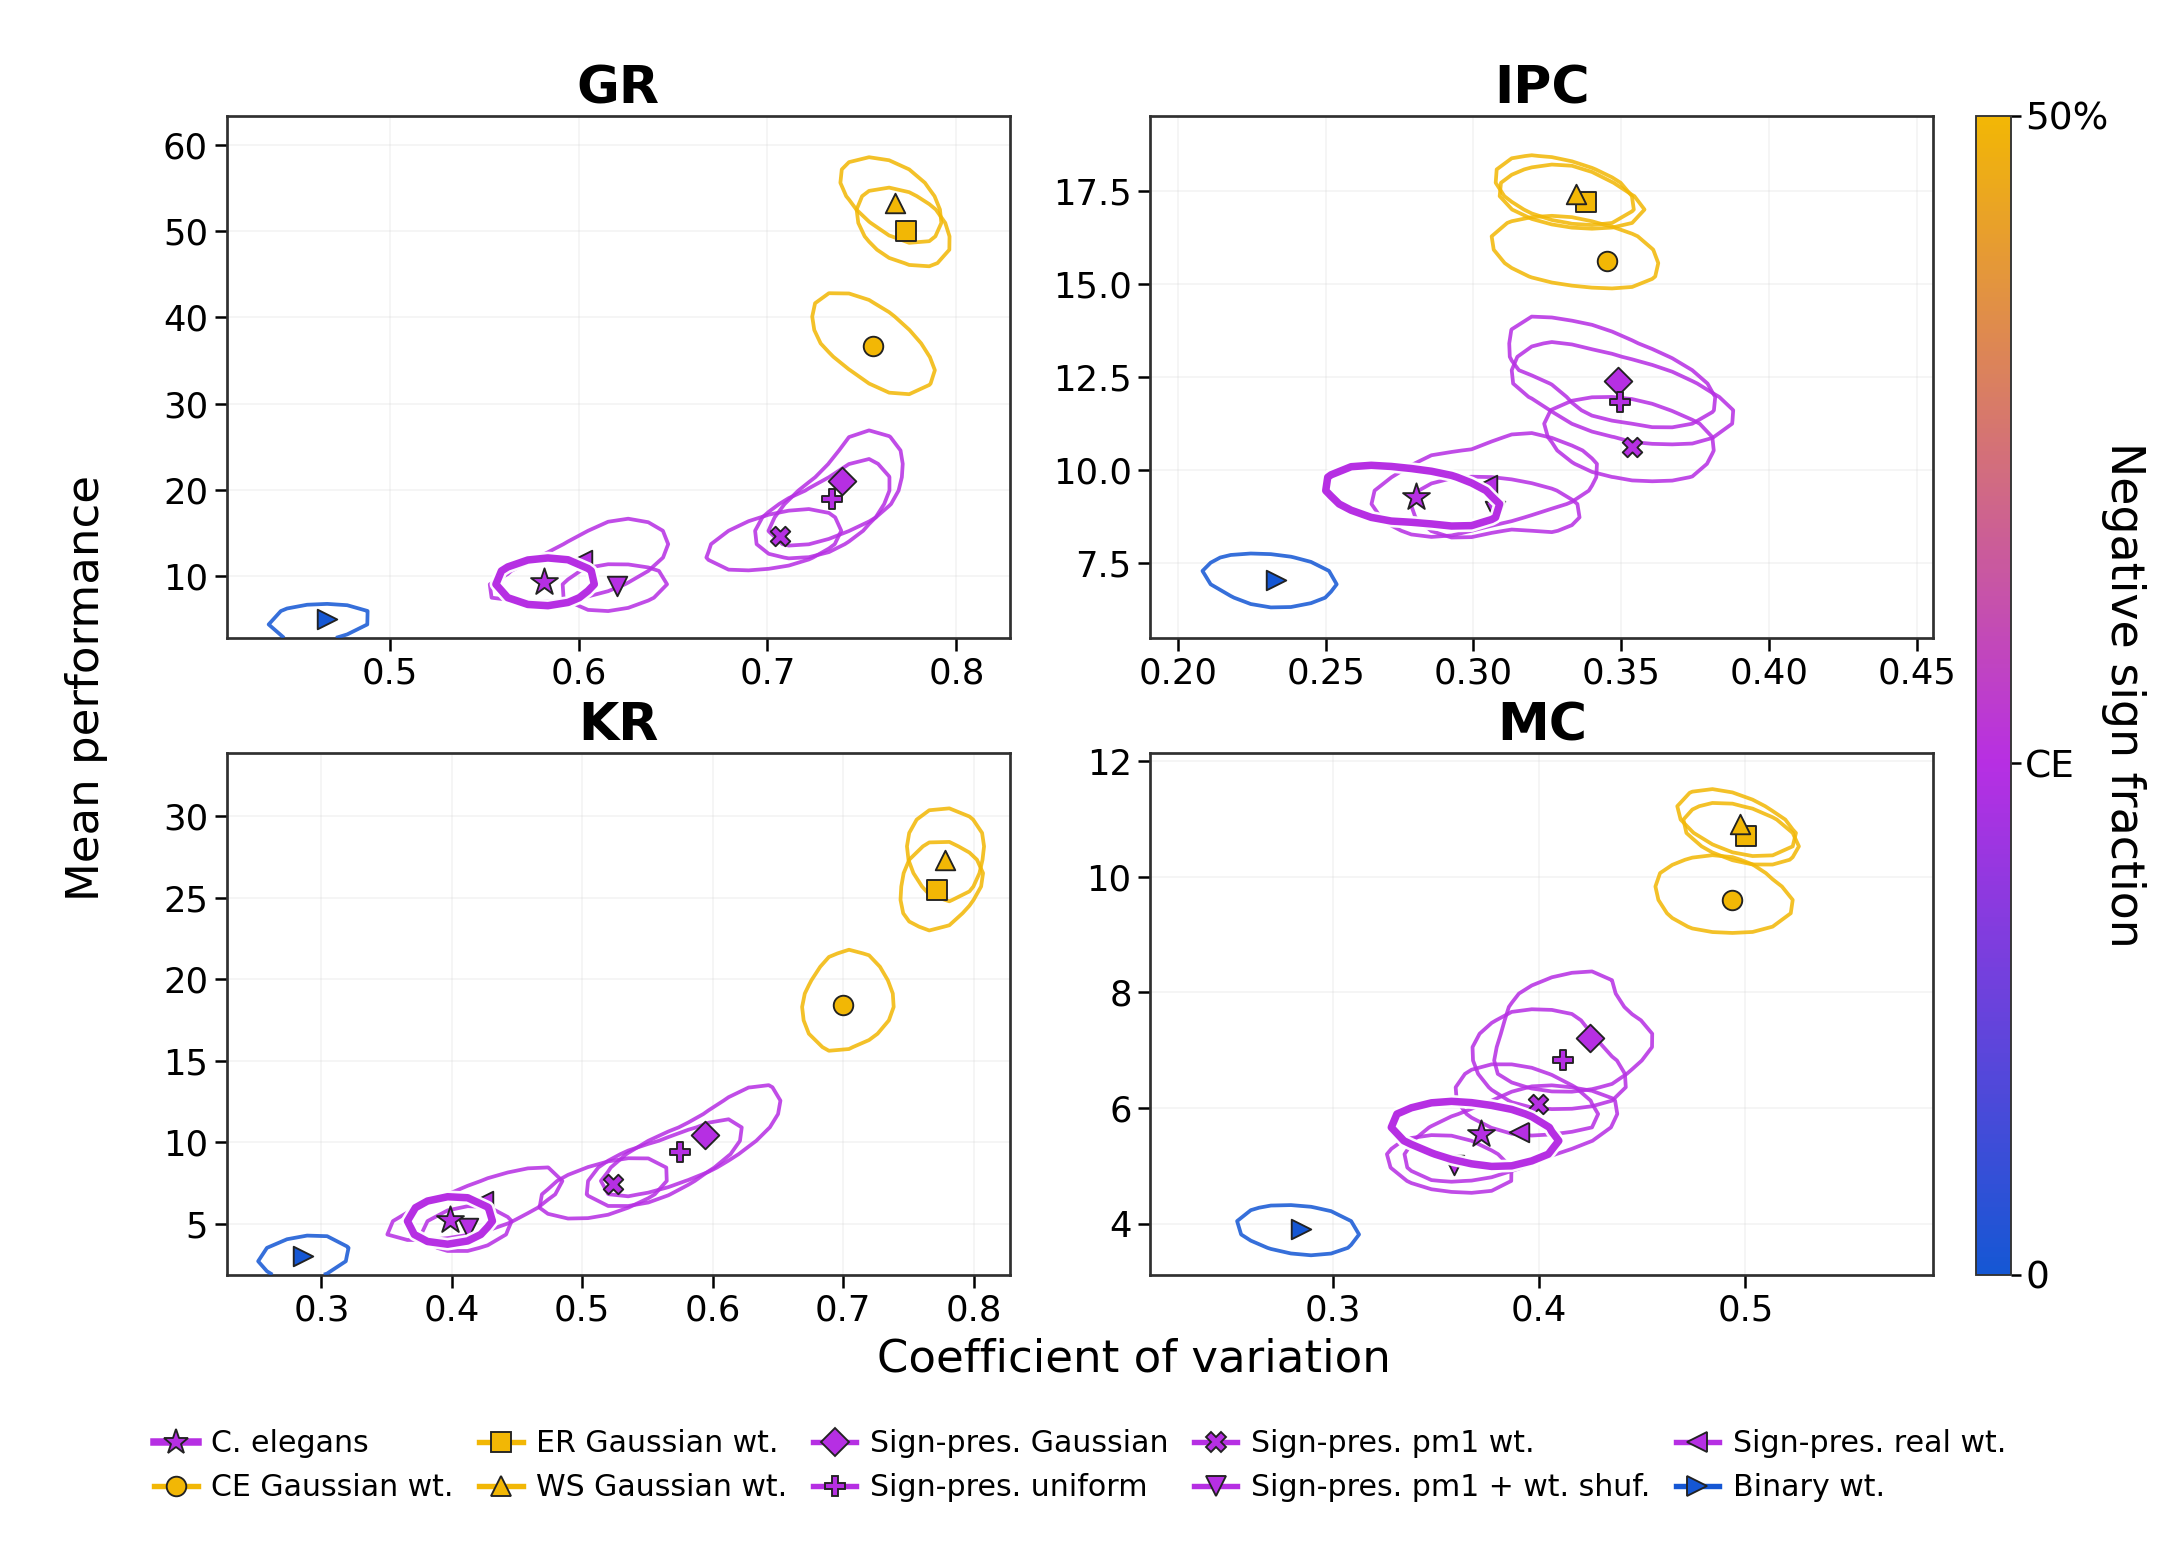
\includegraphics[width=\linewidth]{New_figs/fullv2/50per.png}
    \caption{Performance--CV island plots for the architecture comparison using 50\% density contours. Each panel shows mean performance against hyperparameter CV for one task-agnostic metric. Points mark condition centers; the black starred island marks the empirical \textit{C.\ elegans} connectome.}
    \label{fig:arch}
\end{figure}

\subsection[Global sign balance reveals a performance-invariance tradeoff]{Global sign balance reveals a performance--invariance tradeoff}
\label{balance}
To isolate global sign balance, we flipped the signs of randomly selected synapses while preserving the remaining structure of each network. This manipulation changes the inhibitory fraction while holding connectivity and, where applicable, magnitudes fixed. It therefore tests how much of the low-variance regime in Figure~\ref{fig:arch} can be recovered from the empirical network's strongly imbalanced E/I sign ratio under otherwise matched conditions.

The result is a clear performance--invariance tradeoff. In the all-positive or strongly sign-imbalanced regime, reservoirs have low CV but reduced mean computational performance. As the inhibitory fraction increases toward a more balanced E/I regime, mean metric values generally rise, but CV rises as well (Figures~\ref{fig:bin_cel_frac_curves},~\ref{fig:er_frac_curves}, and~\ref{fig:og_cel_frac_curves}). Thus, the same manipulation that increases computational capability also makes the reservoir more sensitive to spectral radius, leak rate, input scaling, and neuron bias.

This performance trend is consistent with recent reservoir studies in which balanced or slightly inhibition-dominated regimes outperform excitation-dominated regimes on memory, prediction, and locomotor-pattern tasks \parencite{srinivasan_ei_balance_2025,de_graaf_spinal_inhibition_2025}. The present result extends that framing by emphasizing not only mean performance, but also the accompanying increase in hyperparameter sensitivity.

This pattern explains why preserving the empirical sign ratio recovers much of the connectome's invariance in the architecture comparison. The empirical connectome, under the coarse neurotransmitter-to-sign mapping used here, sits on the low-variance side of the tradeoff rather than near the peak-performance region. In the reservoir-computing abstraction studied here, the approximately 4:1 excitatory-to-inhibitory balance associated with many biological networks does not prioritize peak task-agnostic performance. Instead, it places the reservoir in a lower-performance but more hyperparameter-invariant regime. Thus global E/I sign imbalance is a strong control parameter in this model, but its effect is expressed through the tested topology and magnitude regimes.

\begin{figure} 
    \centering
    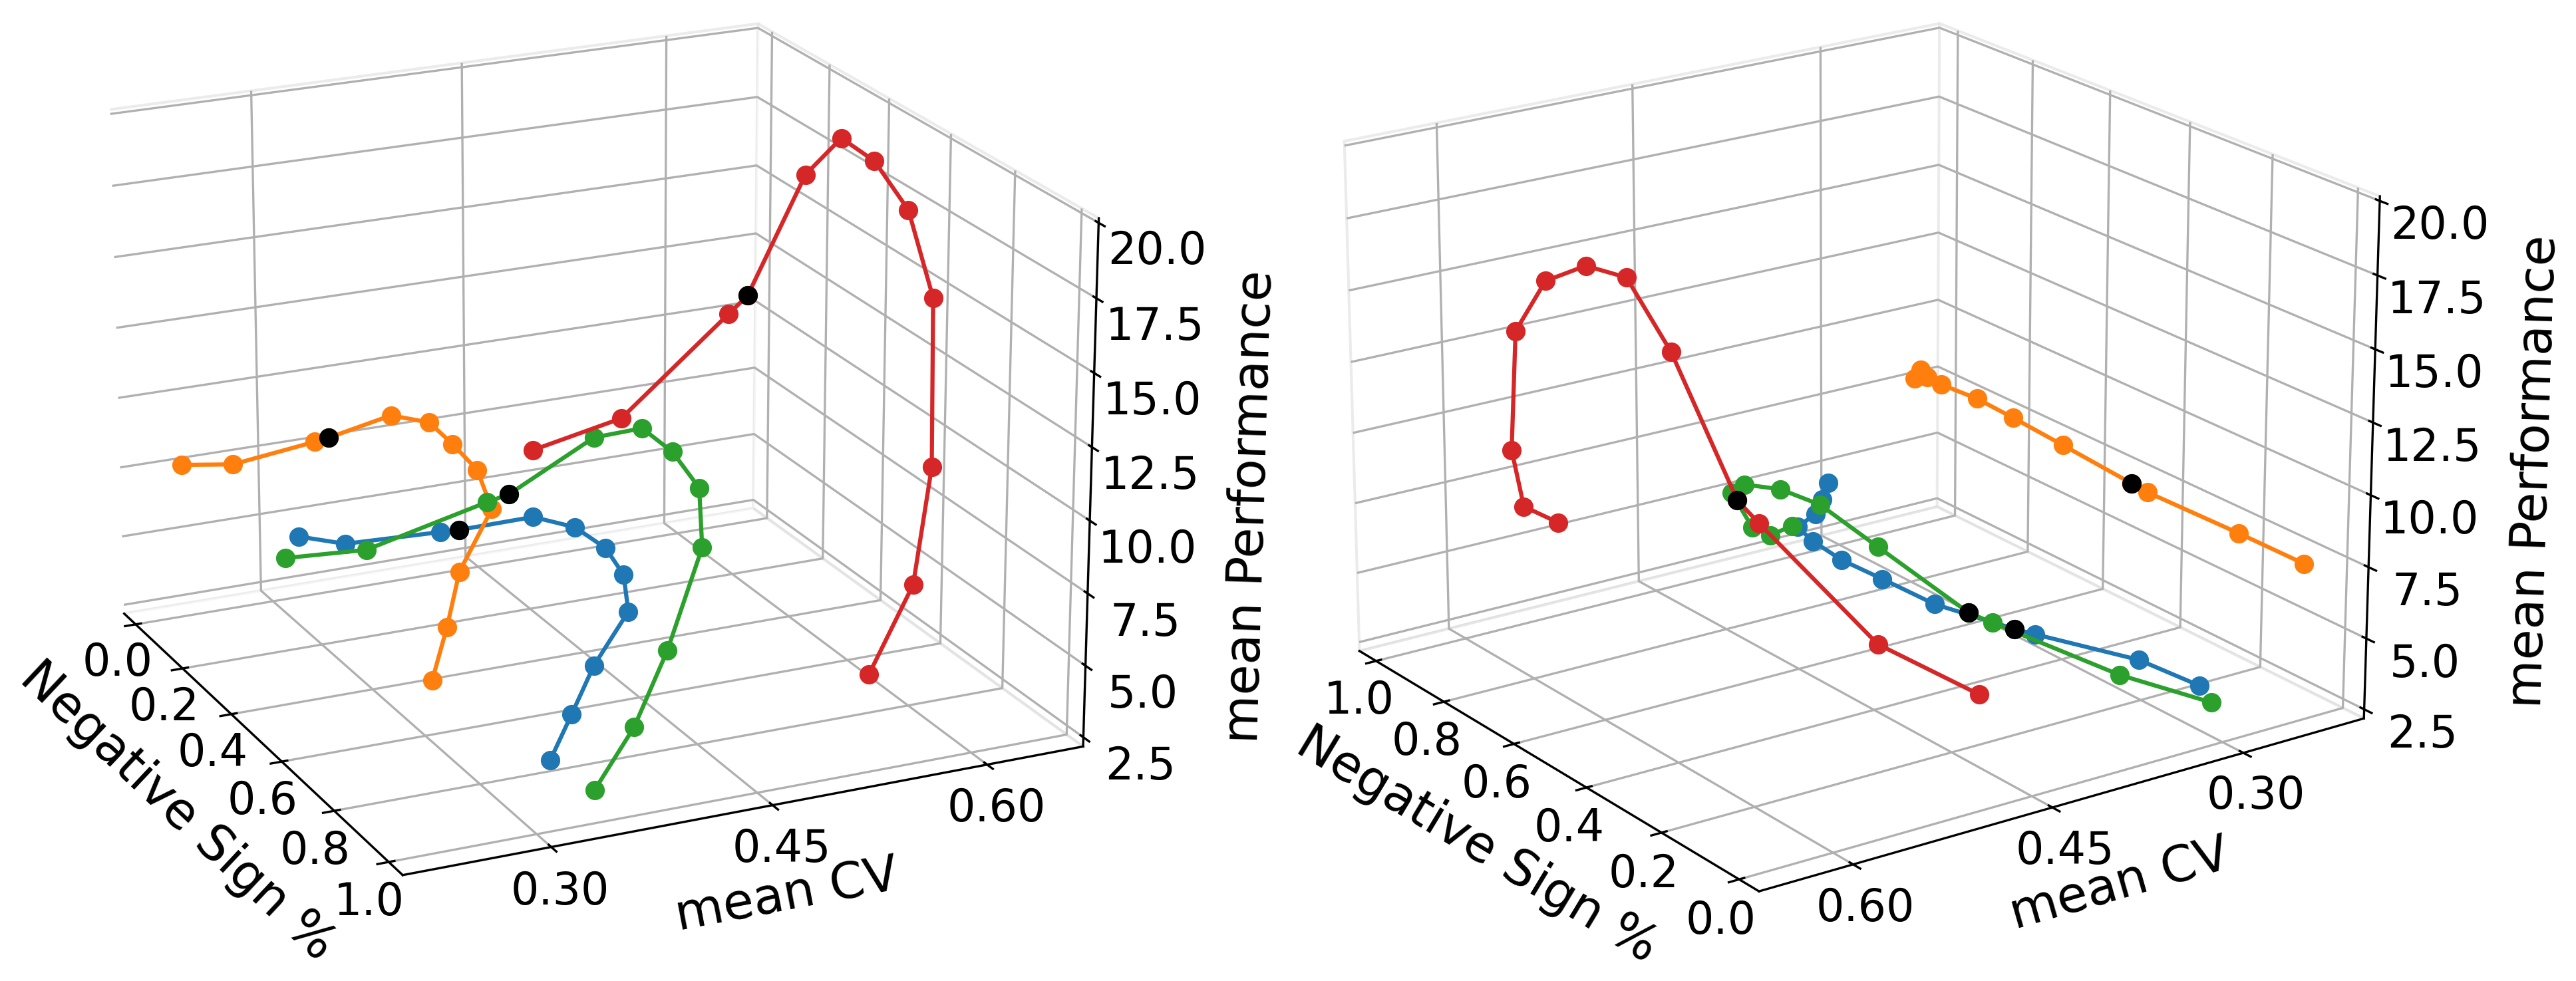
\includegraphics[width=1\linewidth]{New_figs/signtest_final_new/new_4to1/meanpoint_frac_cv_lines.png}
    \caption{Mean performance and mean hyperparameter CV as a function of negative sign percentage for the \textit{C.\ elegans} topology with real weights, using the augmented graph in which complex or unknown neurotransmitter signs are assigned under a 4:1 excitatory-to-inhibitory prior. IPC is denoted in orange, GR in red, MC in blue, and KR in green. Increasing the negative sign percentage moves the reservoir from a low-variance, low-performance regime toward a higher-performance but more hyperparameter-sensitive regime. A total of 50 trials were performed for each fraction.}
    \label{fig:bin_cel_frac_curves}
\end{figure}

\begin{figure}
    \centering
    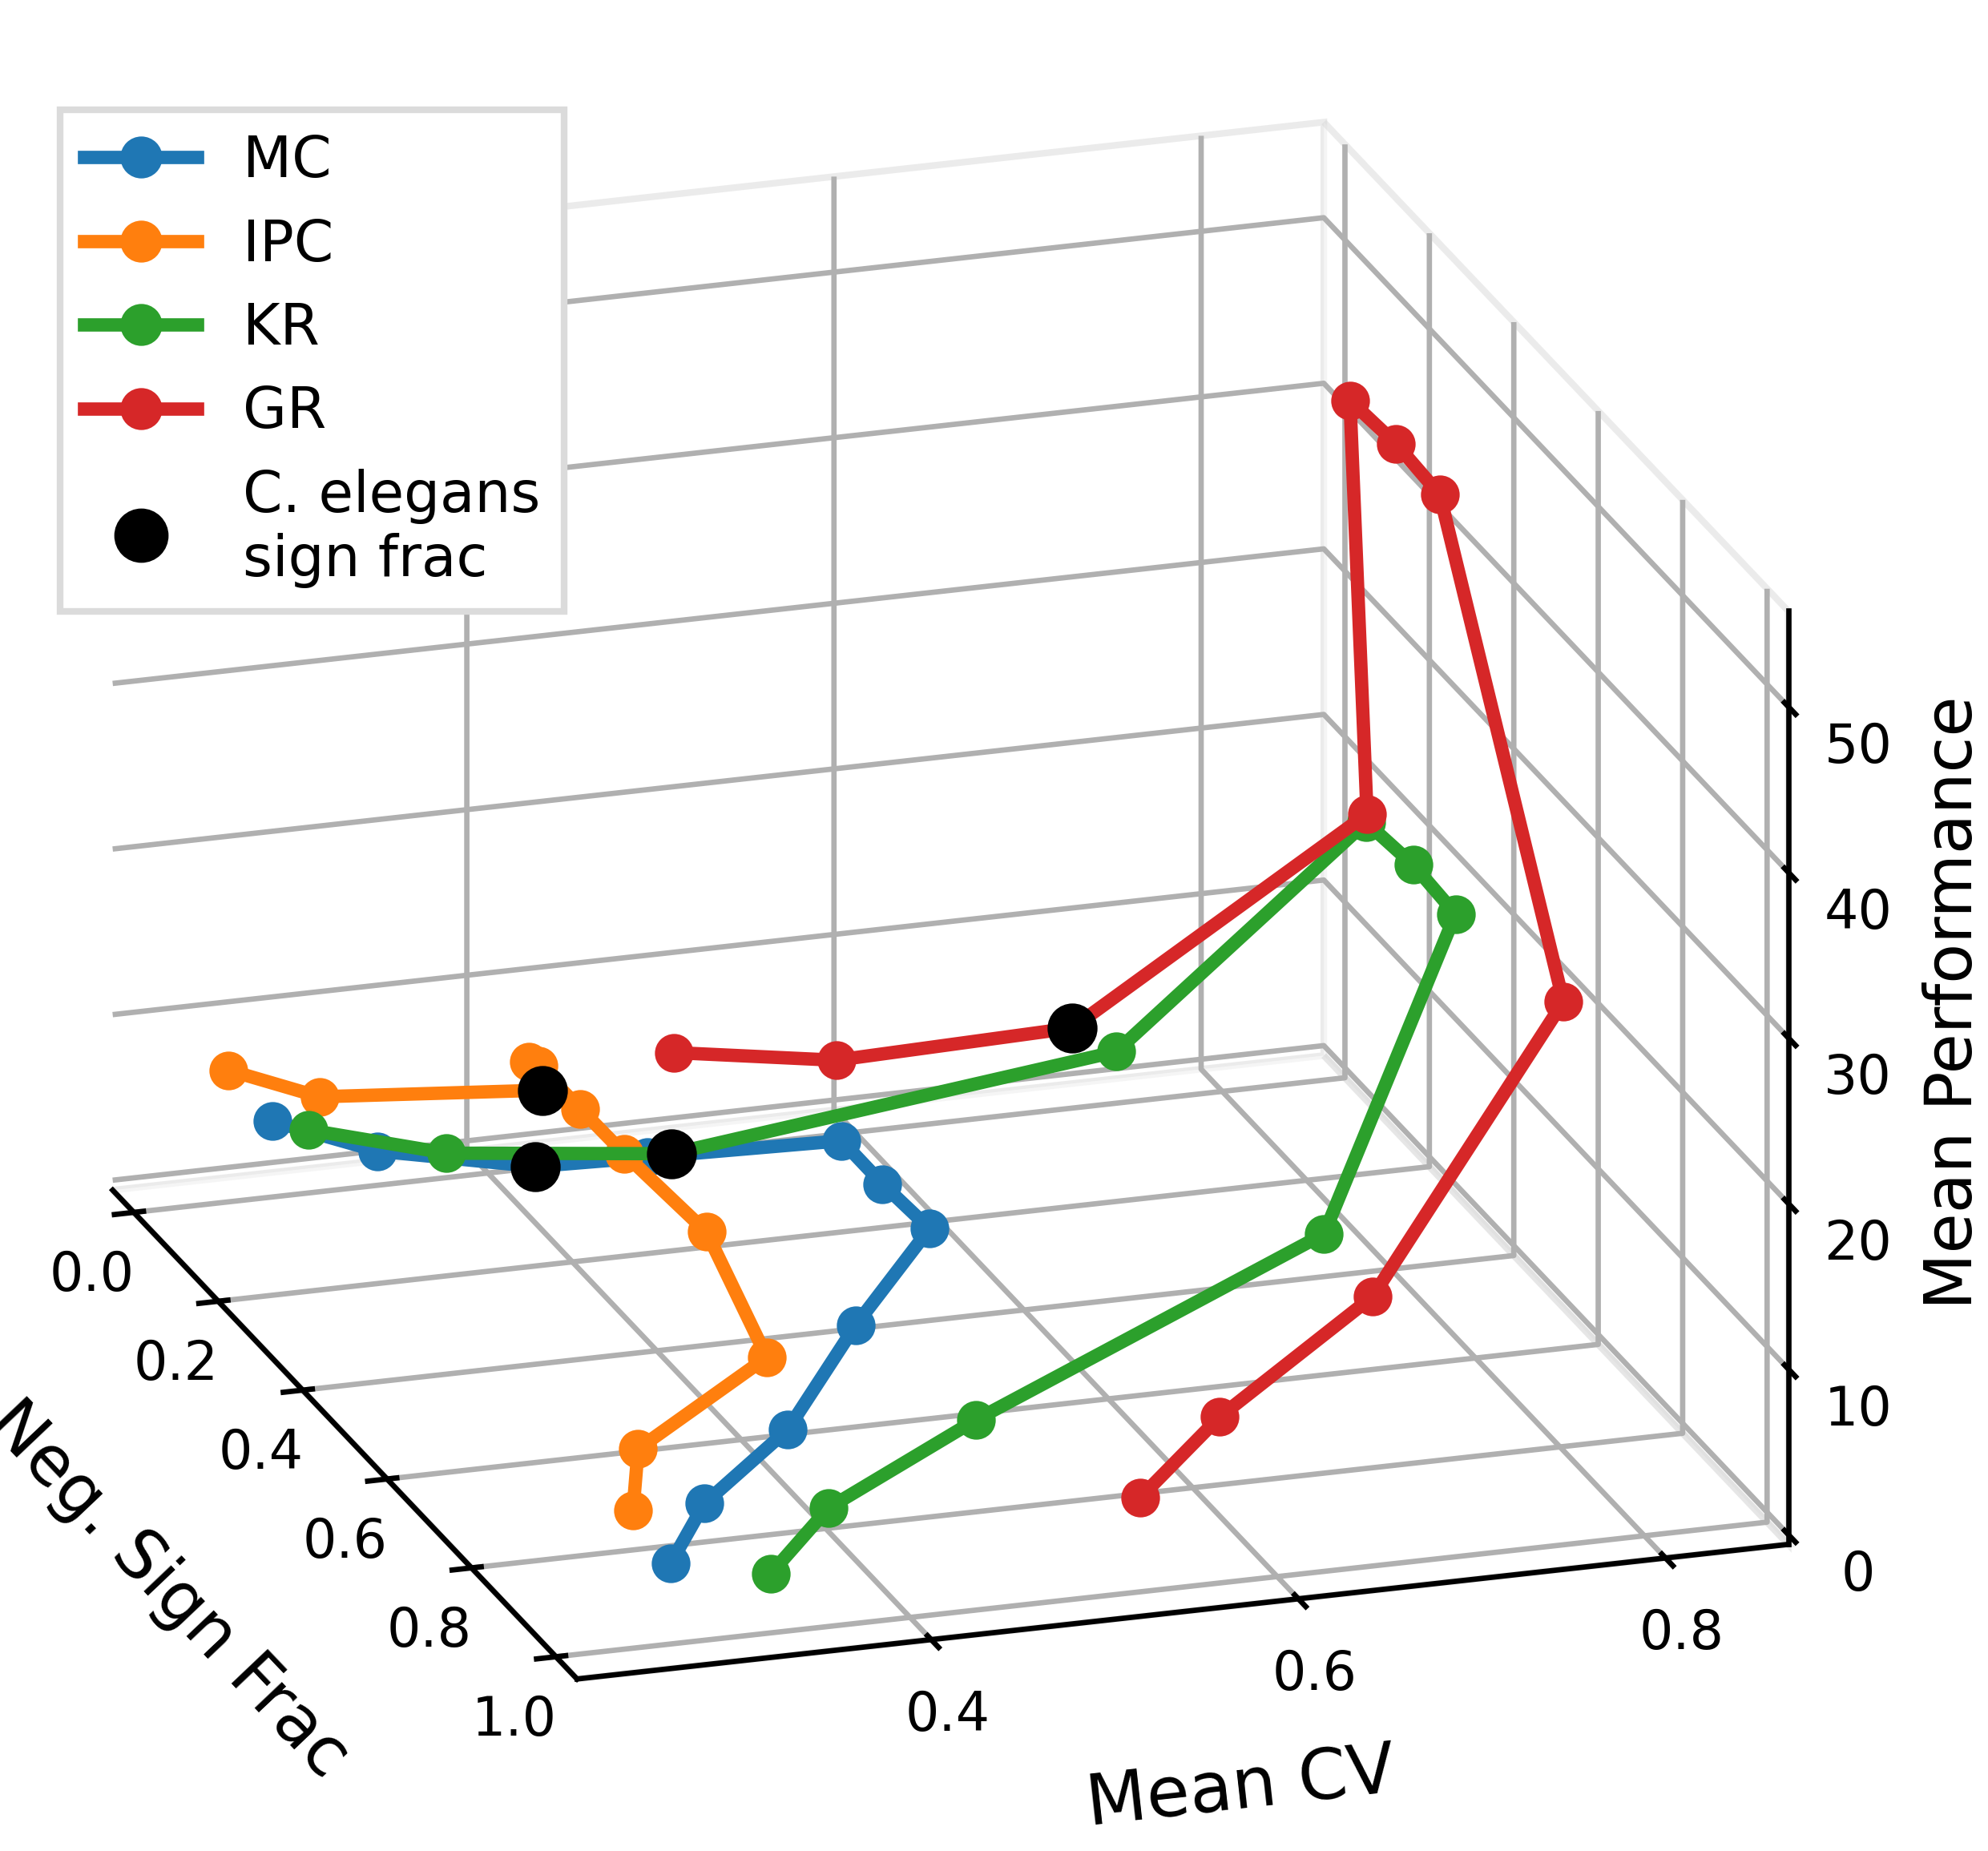
\includegraphics[width=1\linewidth]{New_figs/signtest_final_new/er_matched/meanpoint_frac_cv_lines.png}
    \caption{Mean performance and mean hyperparameter CV as a function of negative sign percentage for the \textit{C.\ elegans}-matched ER topology. IPC is denoted in orange, GR in red, MC in blue, and KR in green. The same performance--invariance tradeoff appears without the biological topology, indicating that global sign balance can act as a primary control parameter within this matched random-topology setting. A total of 50 trials were performed for each fraction.}
    \label{fig:er_frac_curves}
\end{figure}

\begin{figure}
    \centering
    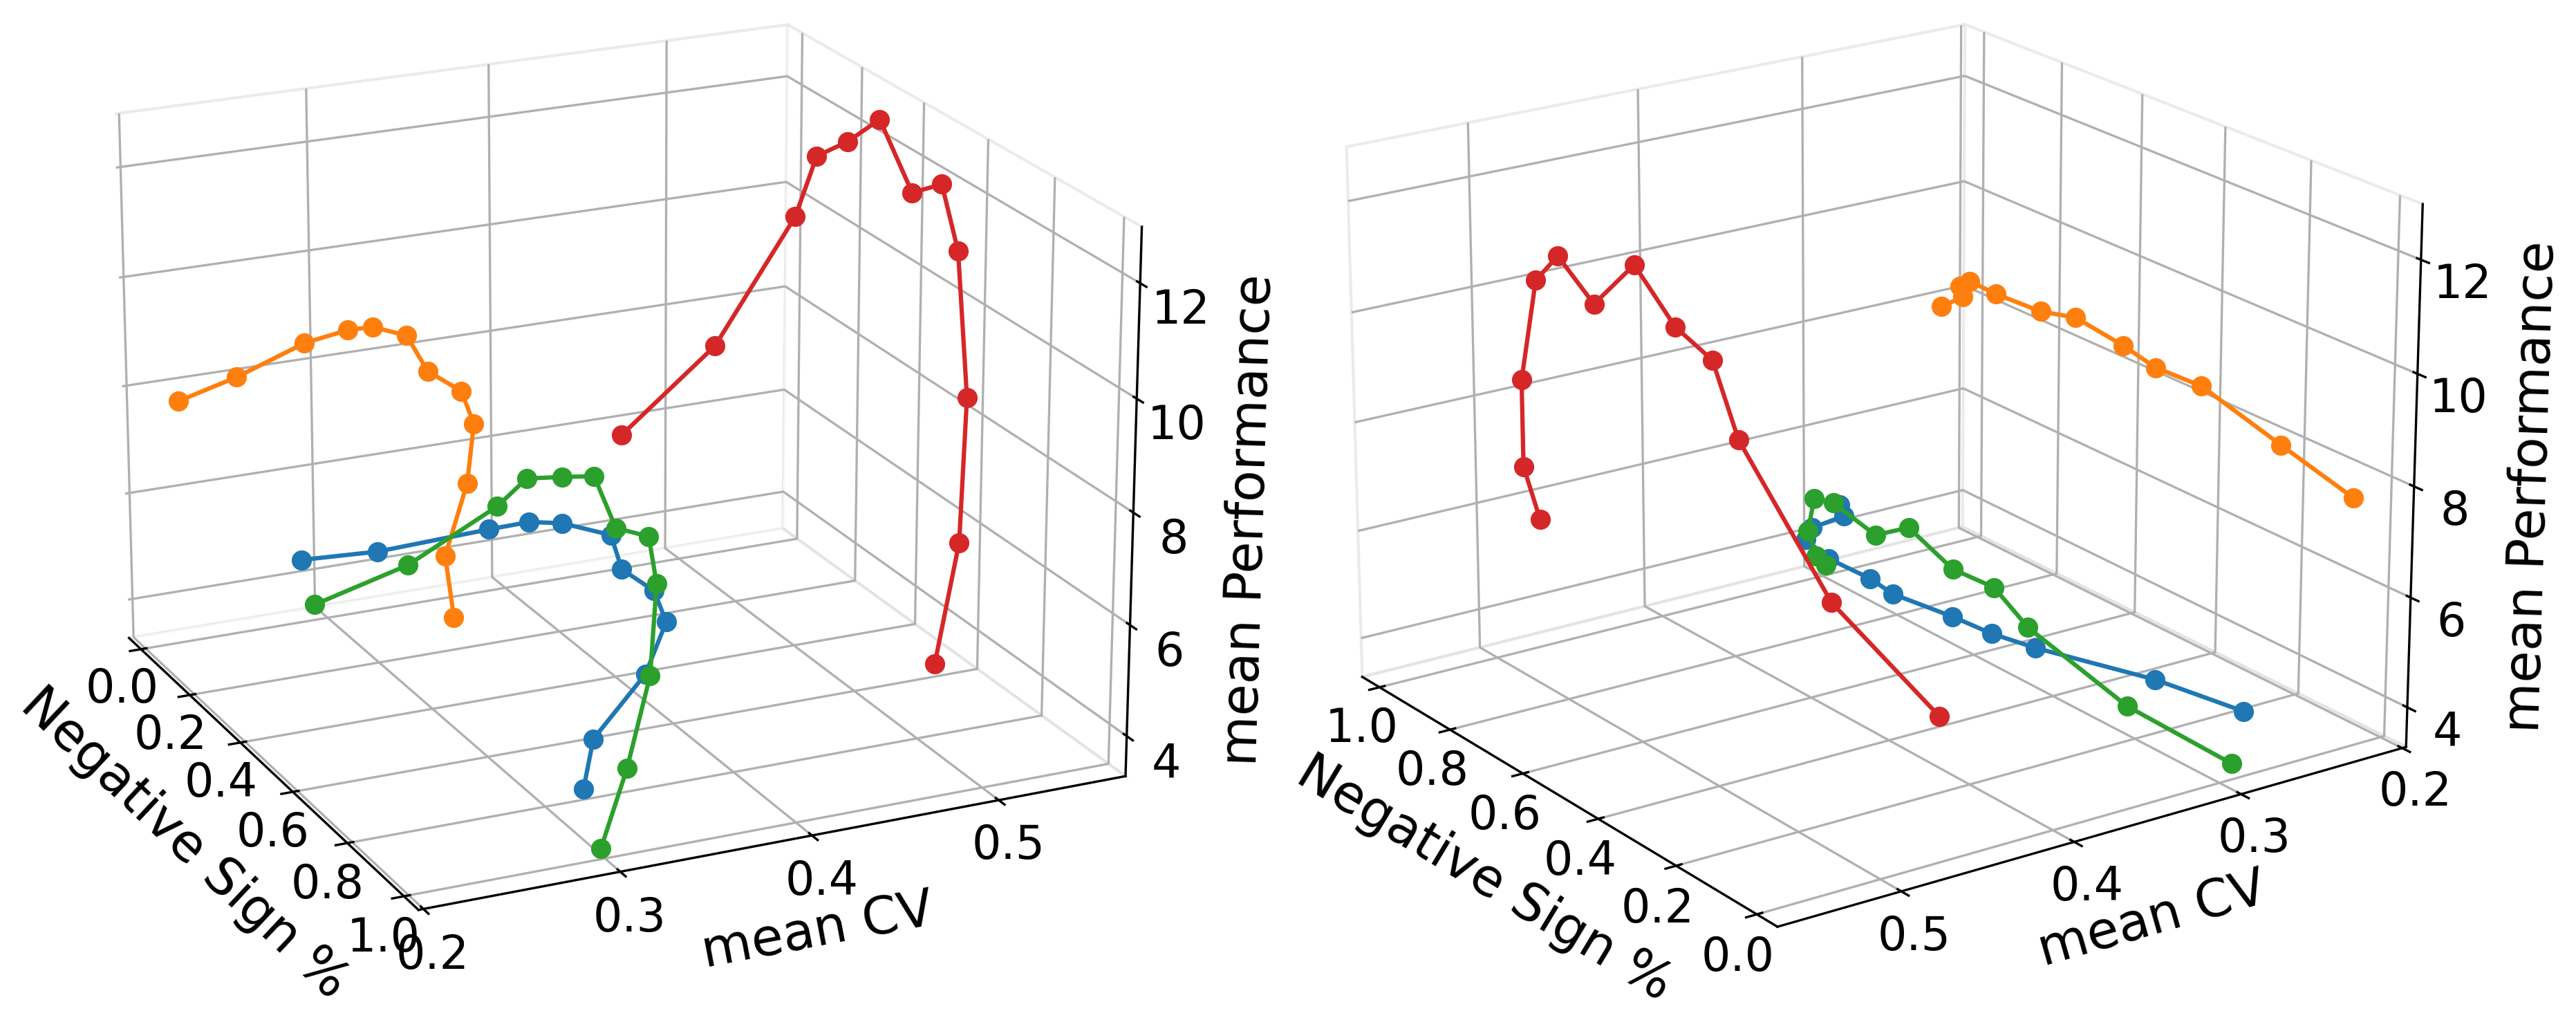
\includegraphics[width=1\linewidth]{New_figs/signtest_final_new/new_removed/meanpoint_frac_cv_lines.png}
    \caption{Mean performance and mean hyperparameter CV as a function of negative sign percentage for the empirical \textit{C.\ elegans} magnitude pattern after removing connections with unknown or complex signs. IPC is denoted in orange, GR in red, MC in blue, and KR in green. Reintroducing inhibitory signs again traces the performance--invariance tradeoff, now with empirical magnitudes held in place. A total of 50 trials were performed for each fraction.}
    \label{fig:og_cel_frac_curves}
\end{figure}

\subsection[Sign-normalization links sign balance to spectral-radius scaling]{Sign-normalization links sign balance to spectral-radius scaling}
\label{sec:sign_norm_ablation}
The sign-fraction curves can be interpreted through the way sign balance changes recurrent gain before spectral normalization. Changing the fraction of negative edges changes whether recurrent loops add coherently or cancel. This changes the raw spectral radius and therefore changes the scale factor applied when the reservoir is normalized. The sign-normalization ablations test this mechanism by comparing the usual normalization by each perturbed matrix's spectral radius, \(W/\rho(W)\), with normalization by the original matrix's spectral radius, \(W/\rho(W_{\mathrm{orig}})\).

For the \textit{C.\ elegans} signed-unit topology, the same peaked performance profile and accompanying CV increase remain visible under both normalization conventions (Figure~\ref{fig:sign_norm_matched_cel}). The ER-matched and empirical-magnitude controls show the same qualitative pattern (Figures~\ref{fig:sign_norm_matched_er} and~\ref{fig:sign_norm_removed_cel}). This does not mean spectral radius is irrelevant. Rather, it shows that sign balance changes the reservoir through the spectral structure that determines normalization and effective recurrent weight scale. Negative signs suppress runaway positive loops; more balanced sign mixtures permit stronger recurrent amplification before normalization and therefore move the reservoir along the performance--invariance tradeoff.

This interpretation is strengthened by recent reservoir-computing work on the no-strong-loops principle in cortical networks. Hadaeghi and colleagues systematically increase link and weight reciprocity and find that stronger direct loops raise the raw spectral radius and reduce memory capacity and kernel rank across synthetic and empirical directed connectomes \parencite{hadaeghi_no_strong_loops_2025}. Their key mechanistic point is directly relevant here: reciprocal motifs inflate \(\rho(W)\), so spectral-radius normalization must suppress the recurrent weights more strongly, lowering the effective average connection strength and narrowing the usable dynamical range. Their manipulation targets reciprocity rather than E/I sign balance, but the overlap is substantial. They alter spectral radius by adding strong loops; here, sign balance alters spectral radius by determining whether loops reinforce or cancel through inhibitory signs.

\begin{figure}
    \centering
    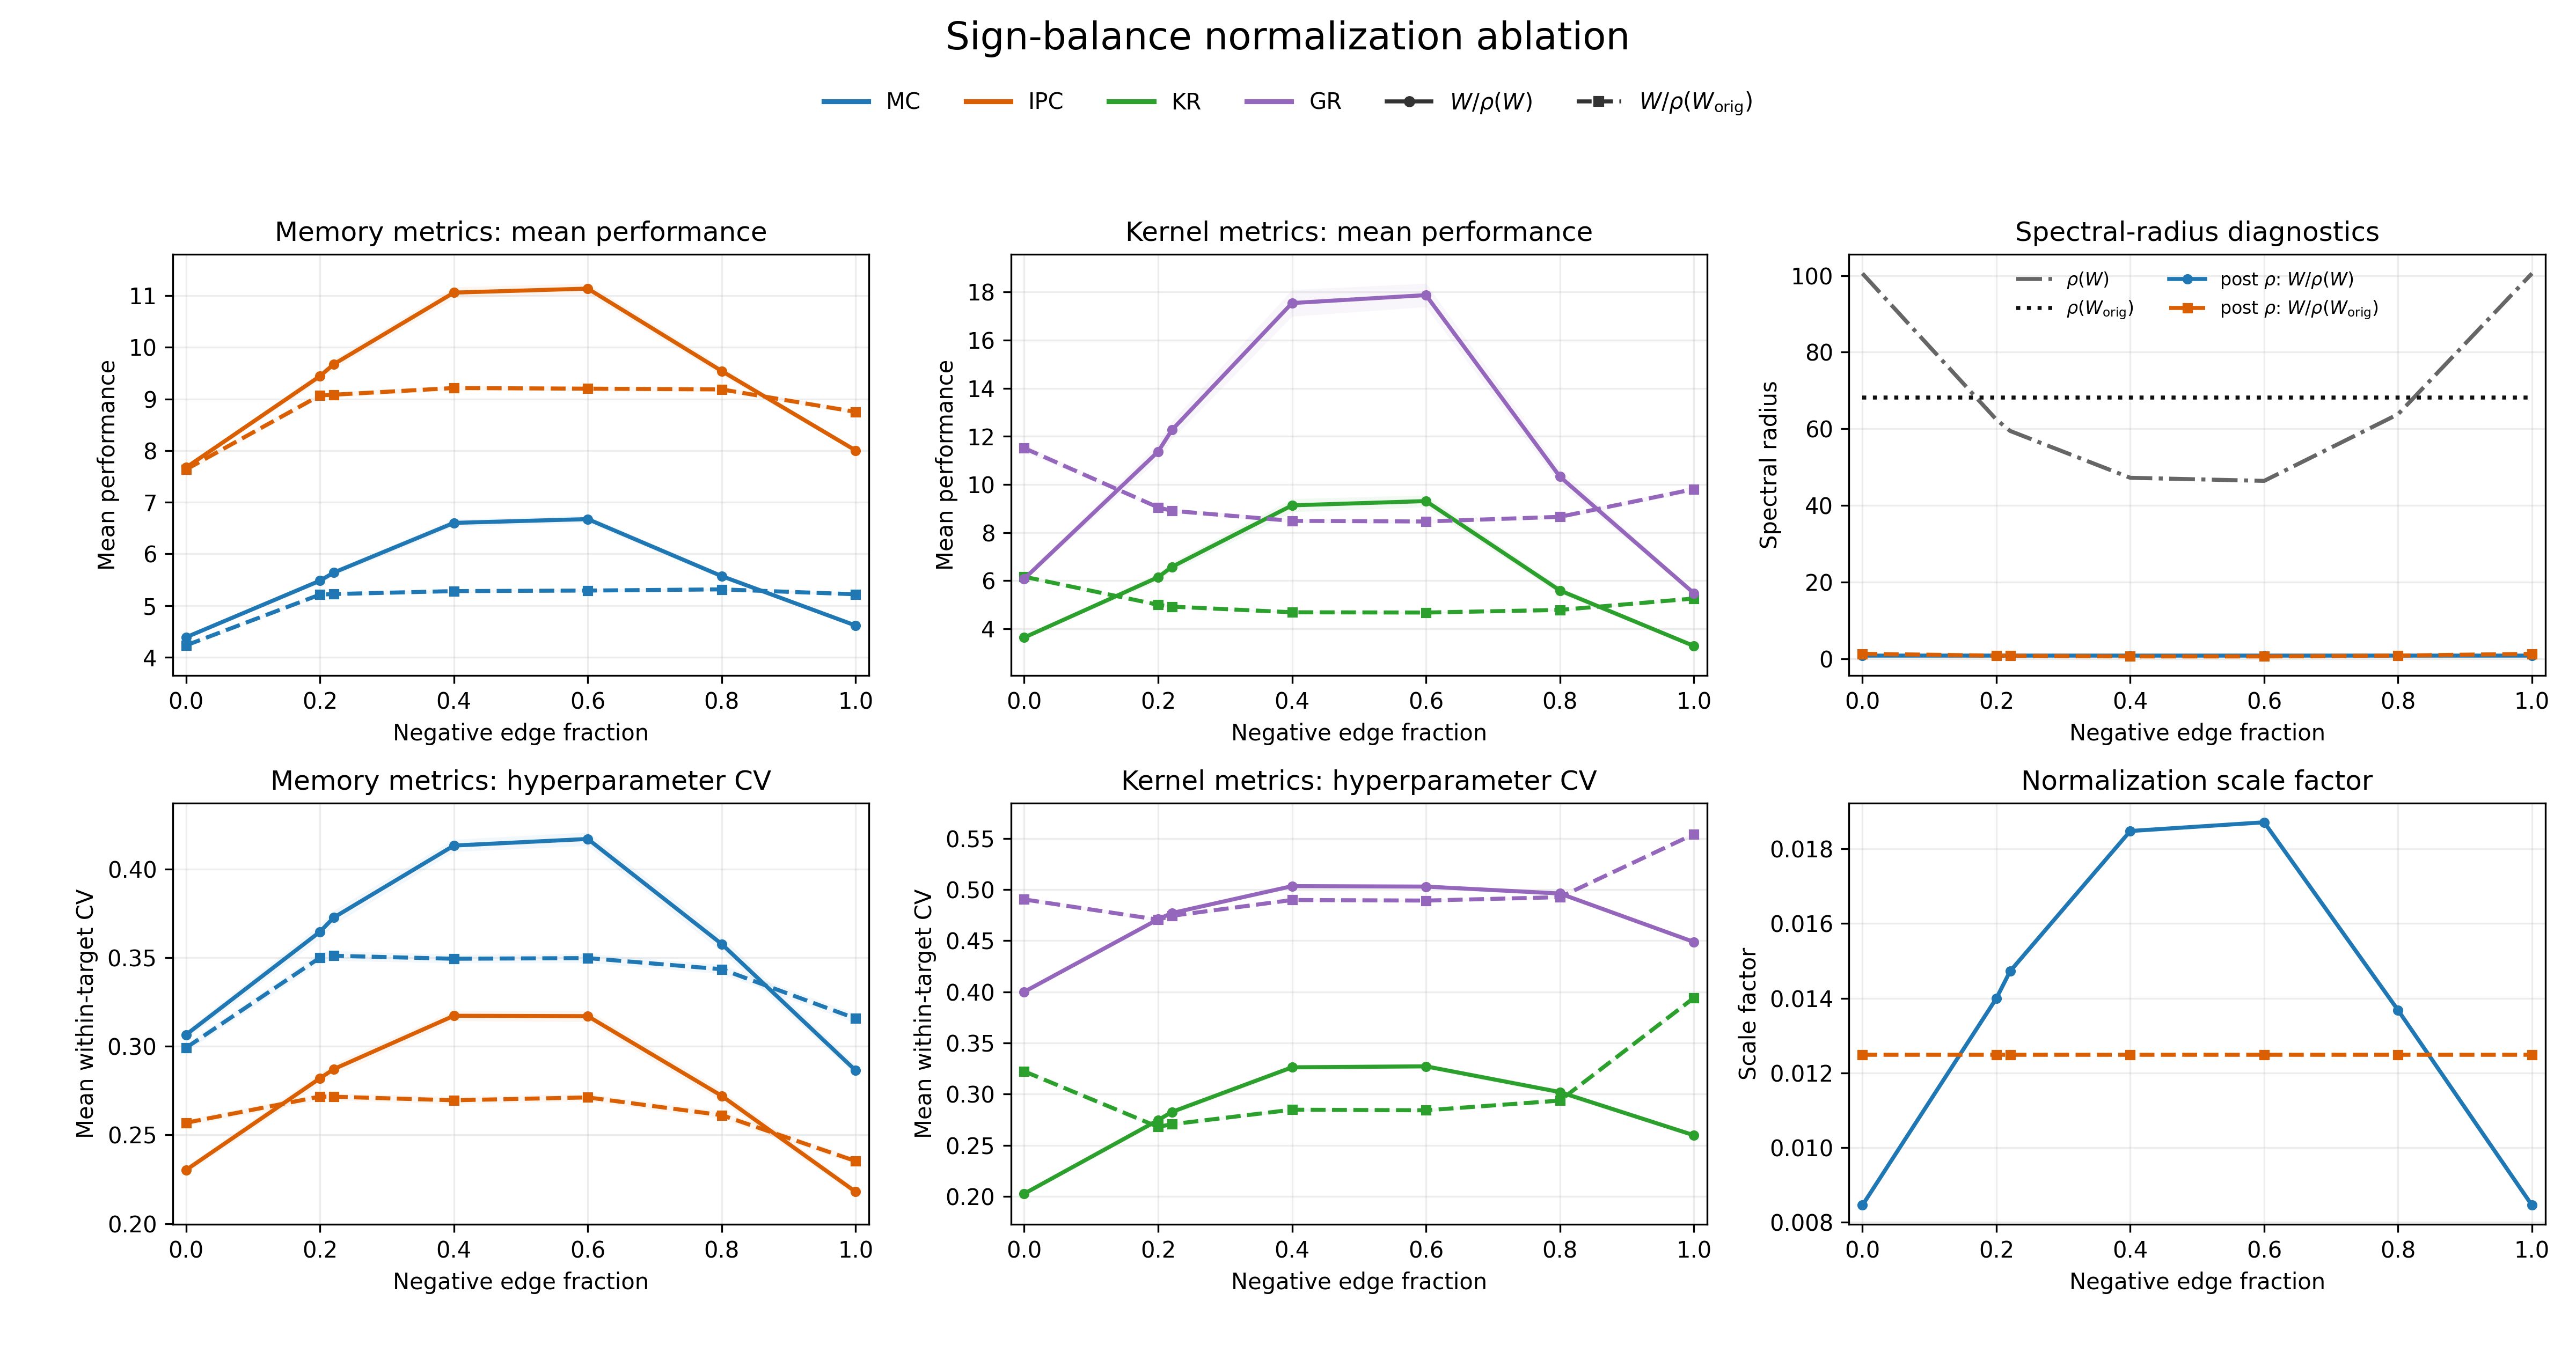
\includegraphics[width=\linewidth]{New_figs/sign_norm_abalation/matched_cel/sign_norm_ablation_combined.png}
    \caption{Sign-balance normalization ablation for the \textit{C.\ elegans} signed-unit topology. Solid curves normalize each perturbed matrix by its own spectral radius; dashed curves normalize by the original spectral radius. The performance--CV tradeoff persists under both conventions.}
    \label{fig:sign_norm_matched_cel}
\end{figure}

\begin{figure}
    \centering
    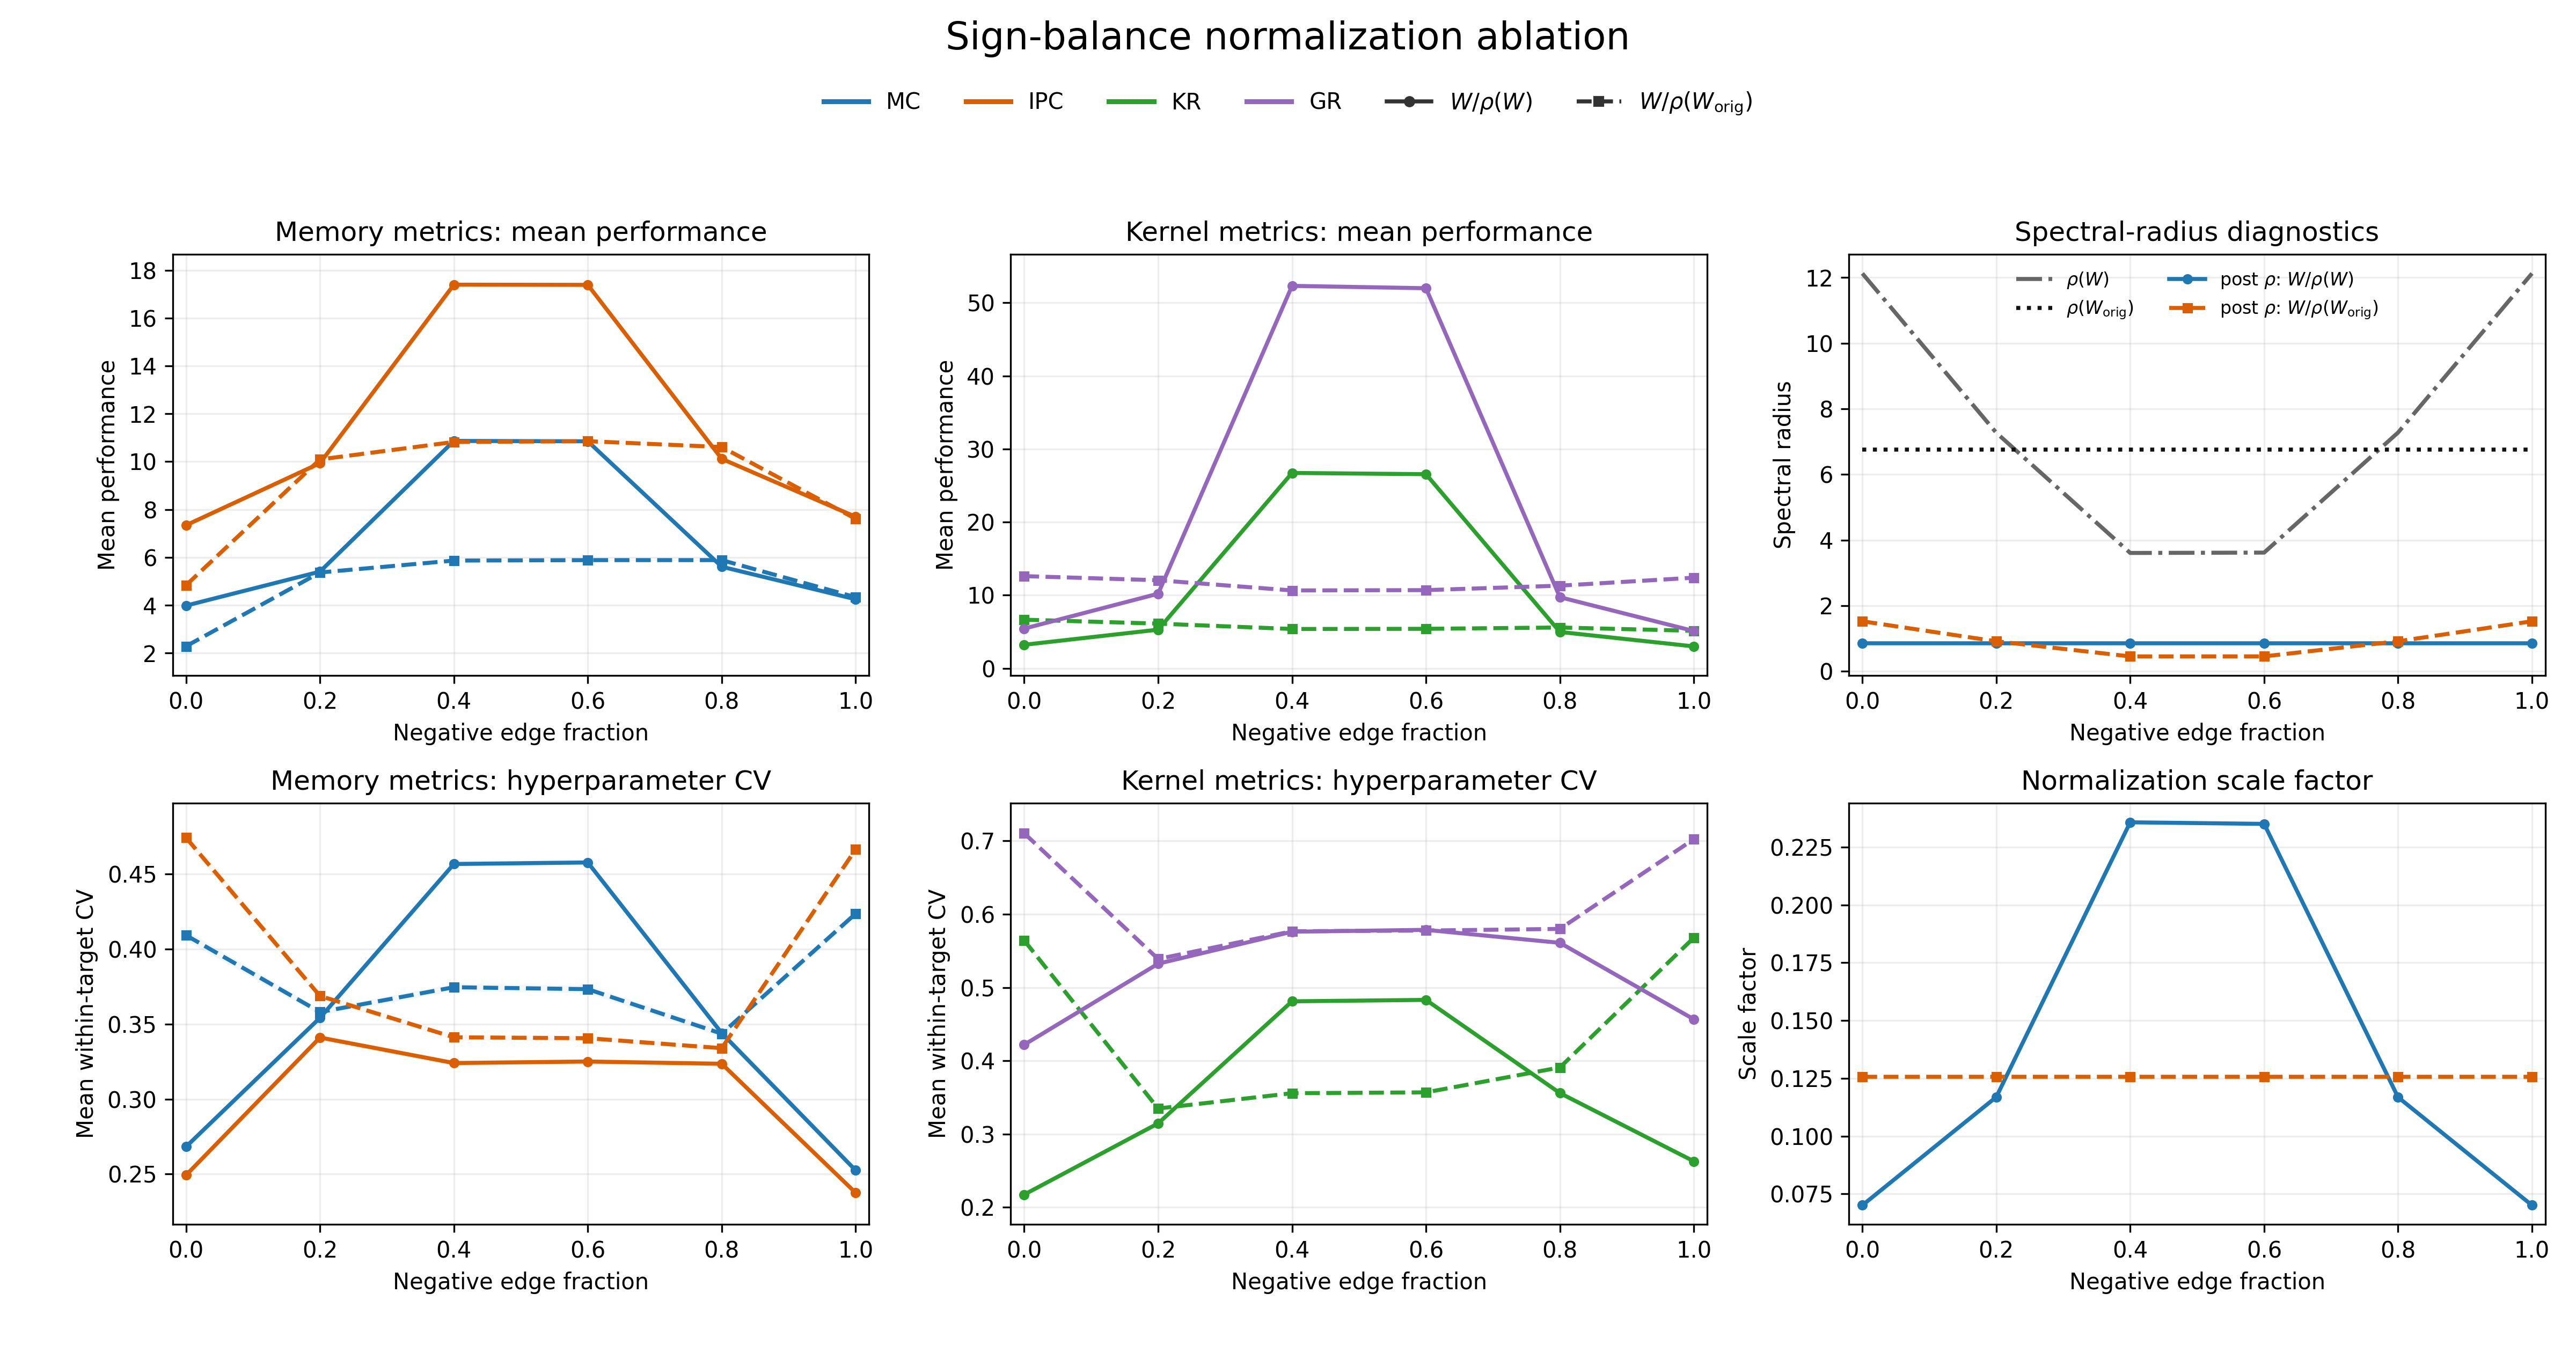
\includegraphics[width=\linewidth]{New_figs/sign_norm_abalation/matched_er/sign_norm_ablation_combined.png}
    \caption{Sign-balance normalization ablation for the \textit{C.\ elegans}-matched ER topology. The same qualitative dependence on negative edge fraction remains after controlling the normalization convention.}
    \label{fig:sign_norm_matched_er}
\end{figure}

\begin{figure}
    \centering
    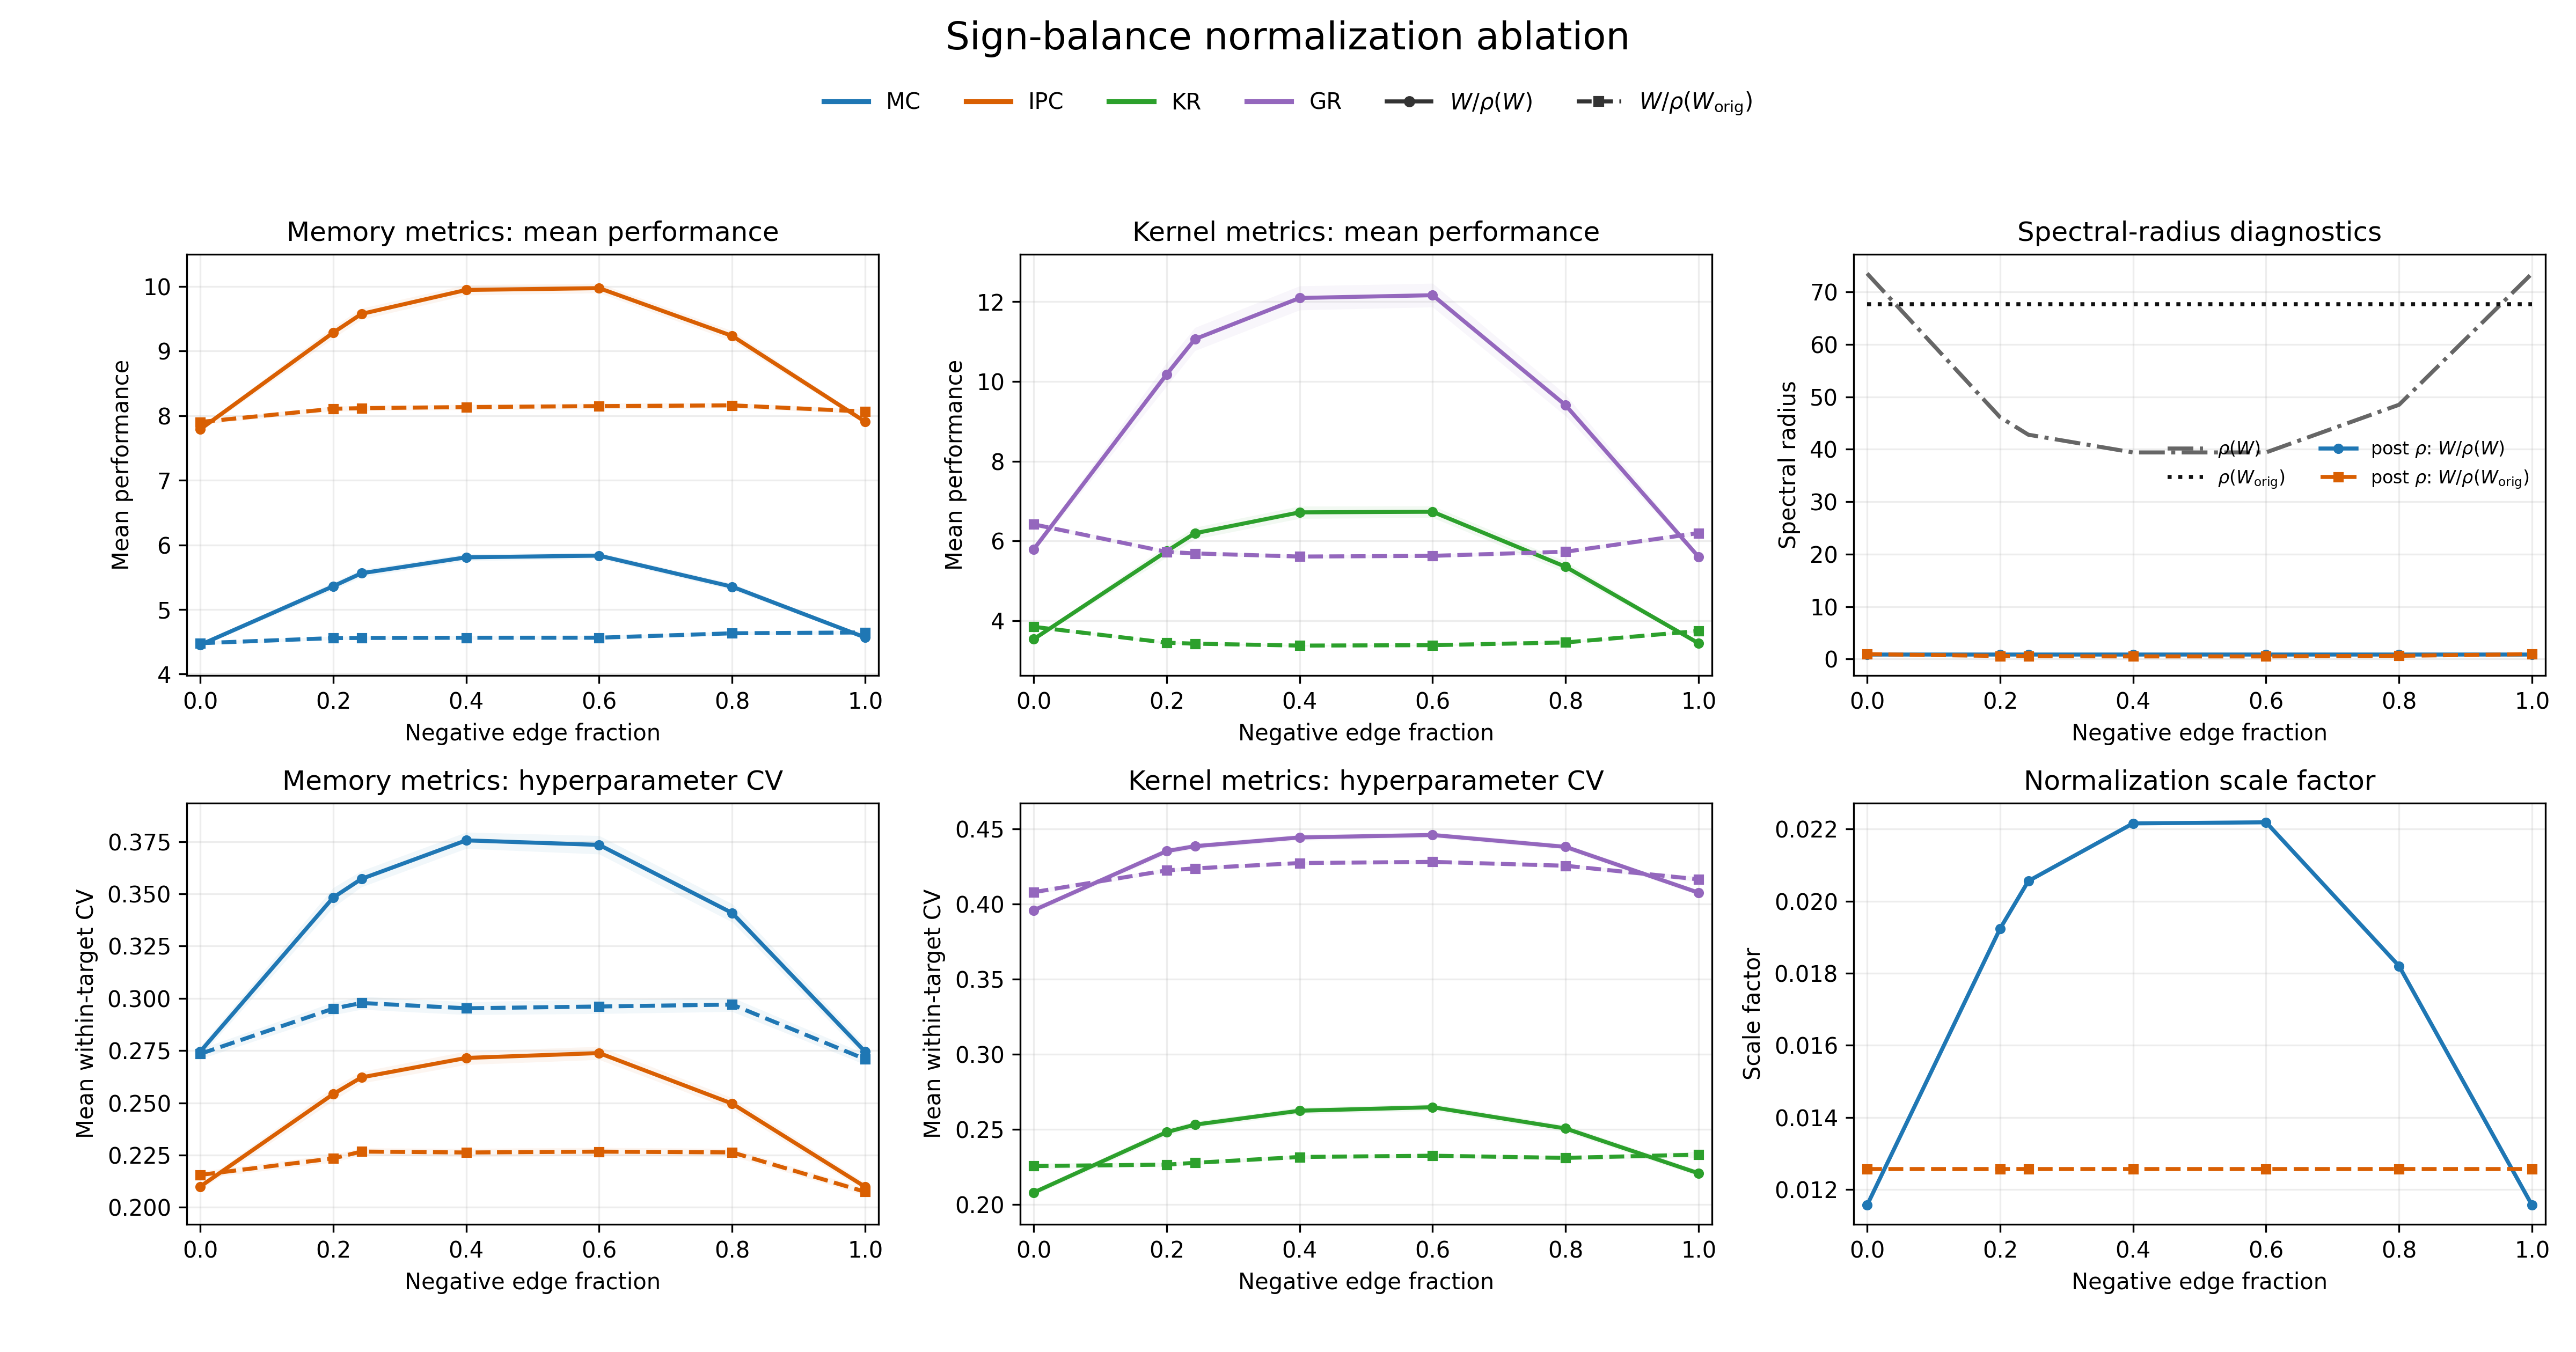
\includegraphics[width=\linewidth]{New_figs/sign_norm_abalation/removed_cel/sign_norm_ablation_combined.png}
    \caption{Sign-balance normalization ablation for the empirical \textit{C.\ elegans} magnitude pattern after removing the original signs. Preserving empirical magnitudes does not eliminate the sign-balance tradeoff.}
    \label{fig:sign_norm_removed_cel}
\end{figure}

\subsection{Topology and heterogeneous magnitudes explain metric-specific residuals}
\label{sec:shuf}
The sign-balance result explains the main architecture-level separation, but it does not explain every metric equally. In the architecture comparison, sign-preserving $\pm 1$ controls recover much of the empirical connectome's invariance for IPC, KR, and GR, but not for MC. By contrast, the sign-preserving Gaussian and uniform controls are closest to the empirical connectome for MC. This indicates that MC depends strongly on heterogeneous weights and their organization on the graph, while the shuffle experiments below show that residual topology and sign-placement effects also appear in KR and GR.

The degree-preserving shuffle experiments sharpen this interpretation. With the original real-valued \textit{C.\ elegans} weights, weight shuffling, connection shuffling, and connection-plus-weight shuffling all move the reservoir away from the unshuffled empirical connectome toward higher mean performance and higher CV (Figure~\ref{fig:realW}). This shift is not explained by magnitude placement alone. Connection shuffling by itself produces CV increases comparable to, and for KR larger than, weight shuffling: relative to the empirical connectome, the connection shuffle increases mean CV by \(18.8\%\) for MC, \(29.8\%\) for IPC, \(50.1\%\) for KR, and \(26.9\%\) for GR (Supplemental Table~\ref{tab:shuffle_cv_real}). The real-weight shuffle results therefore point to an interaction between graph organization, sign placement, and heterogeneous magnitude placement: disrupting either the empirical edge arrangement or the empirical assignment of magnitudes moves the reservoir out of the compact low-variance regime.

When all nonzero weights are collapsed to $\pm 1$ while preserving the empirical sign ratio, the picture changes (Figure~\ref{fig:pm1W}). Using the original local sign placement as the baseline, the sign- and topology-shuffled signed-unit controls have lower CV across all four metrics (Supplemental Table~\ref{tab:shuffle_cv_pm1}). The largest proportional reductions occur for KR: \(-21.2\%\) for sign-preserving weight shuffling, \(-14.0\%\) for connection shuffling, and \(-21.9\%\) for the combined sign-preserving shuffle. Preserving only the global sign ratio therefore recovers a lower-variance regime, but it does not make sign placement irrelevant; the original local sign arrangement places the signed-unit reservoir in a higher-performance, higher-CV regime than the shuffled signed-unit controls. The binary-weight experiment isolates topology further: once every nonzero edge has the same positive sign and magnitude, degree-preserving rewiring lowers CV most for MC (\(-10.2\%\)) and also for KR (\(-5.3\%\)), while IPC changes negligibly and GR changes more weakly (Figure~\ref{fig:bW}; Supplemental Table~\ref{tab:shuffle_cv_binary}).

These results give the hierarchy its second level. Global E/I sign imbalance is the strongest single control of the low-variance regime in the tested \textit{C.\ elegans} reservoir family, especially for IPC, KR, and GR, but the shuffle experiments show that it is not acting alone. Topology, sign placement, and heterogeneous magnitudes determine how far the sign-balance effect carries and where it breaks down. MC is the clearest architecture-level exception to the sign-balance simplification, while KR is especially sensitive to real-weight connection shuffling and signed-unit sign/topology rearrangements.

\begin{figure}
    \centering
    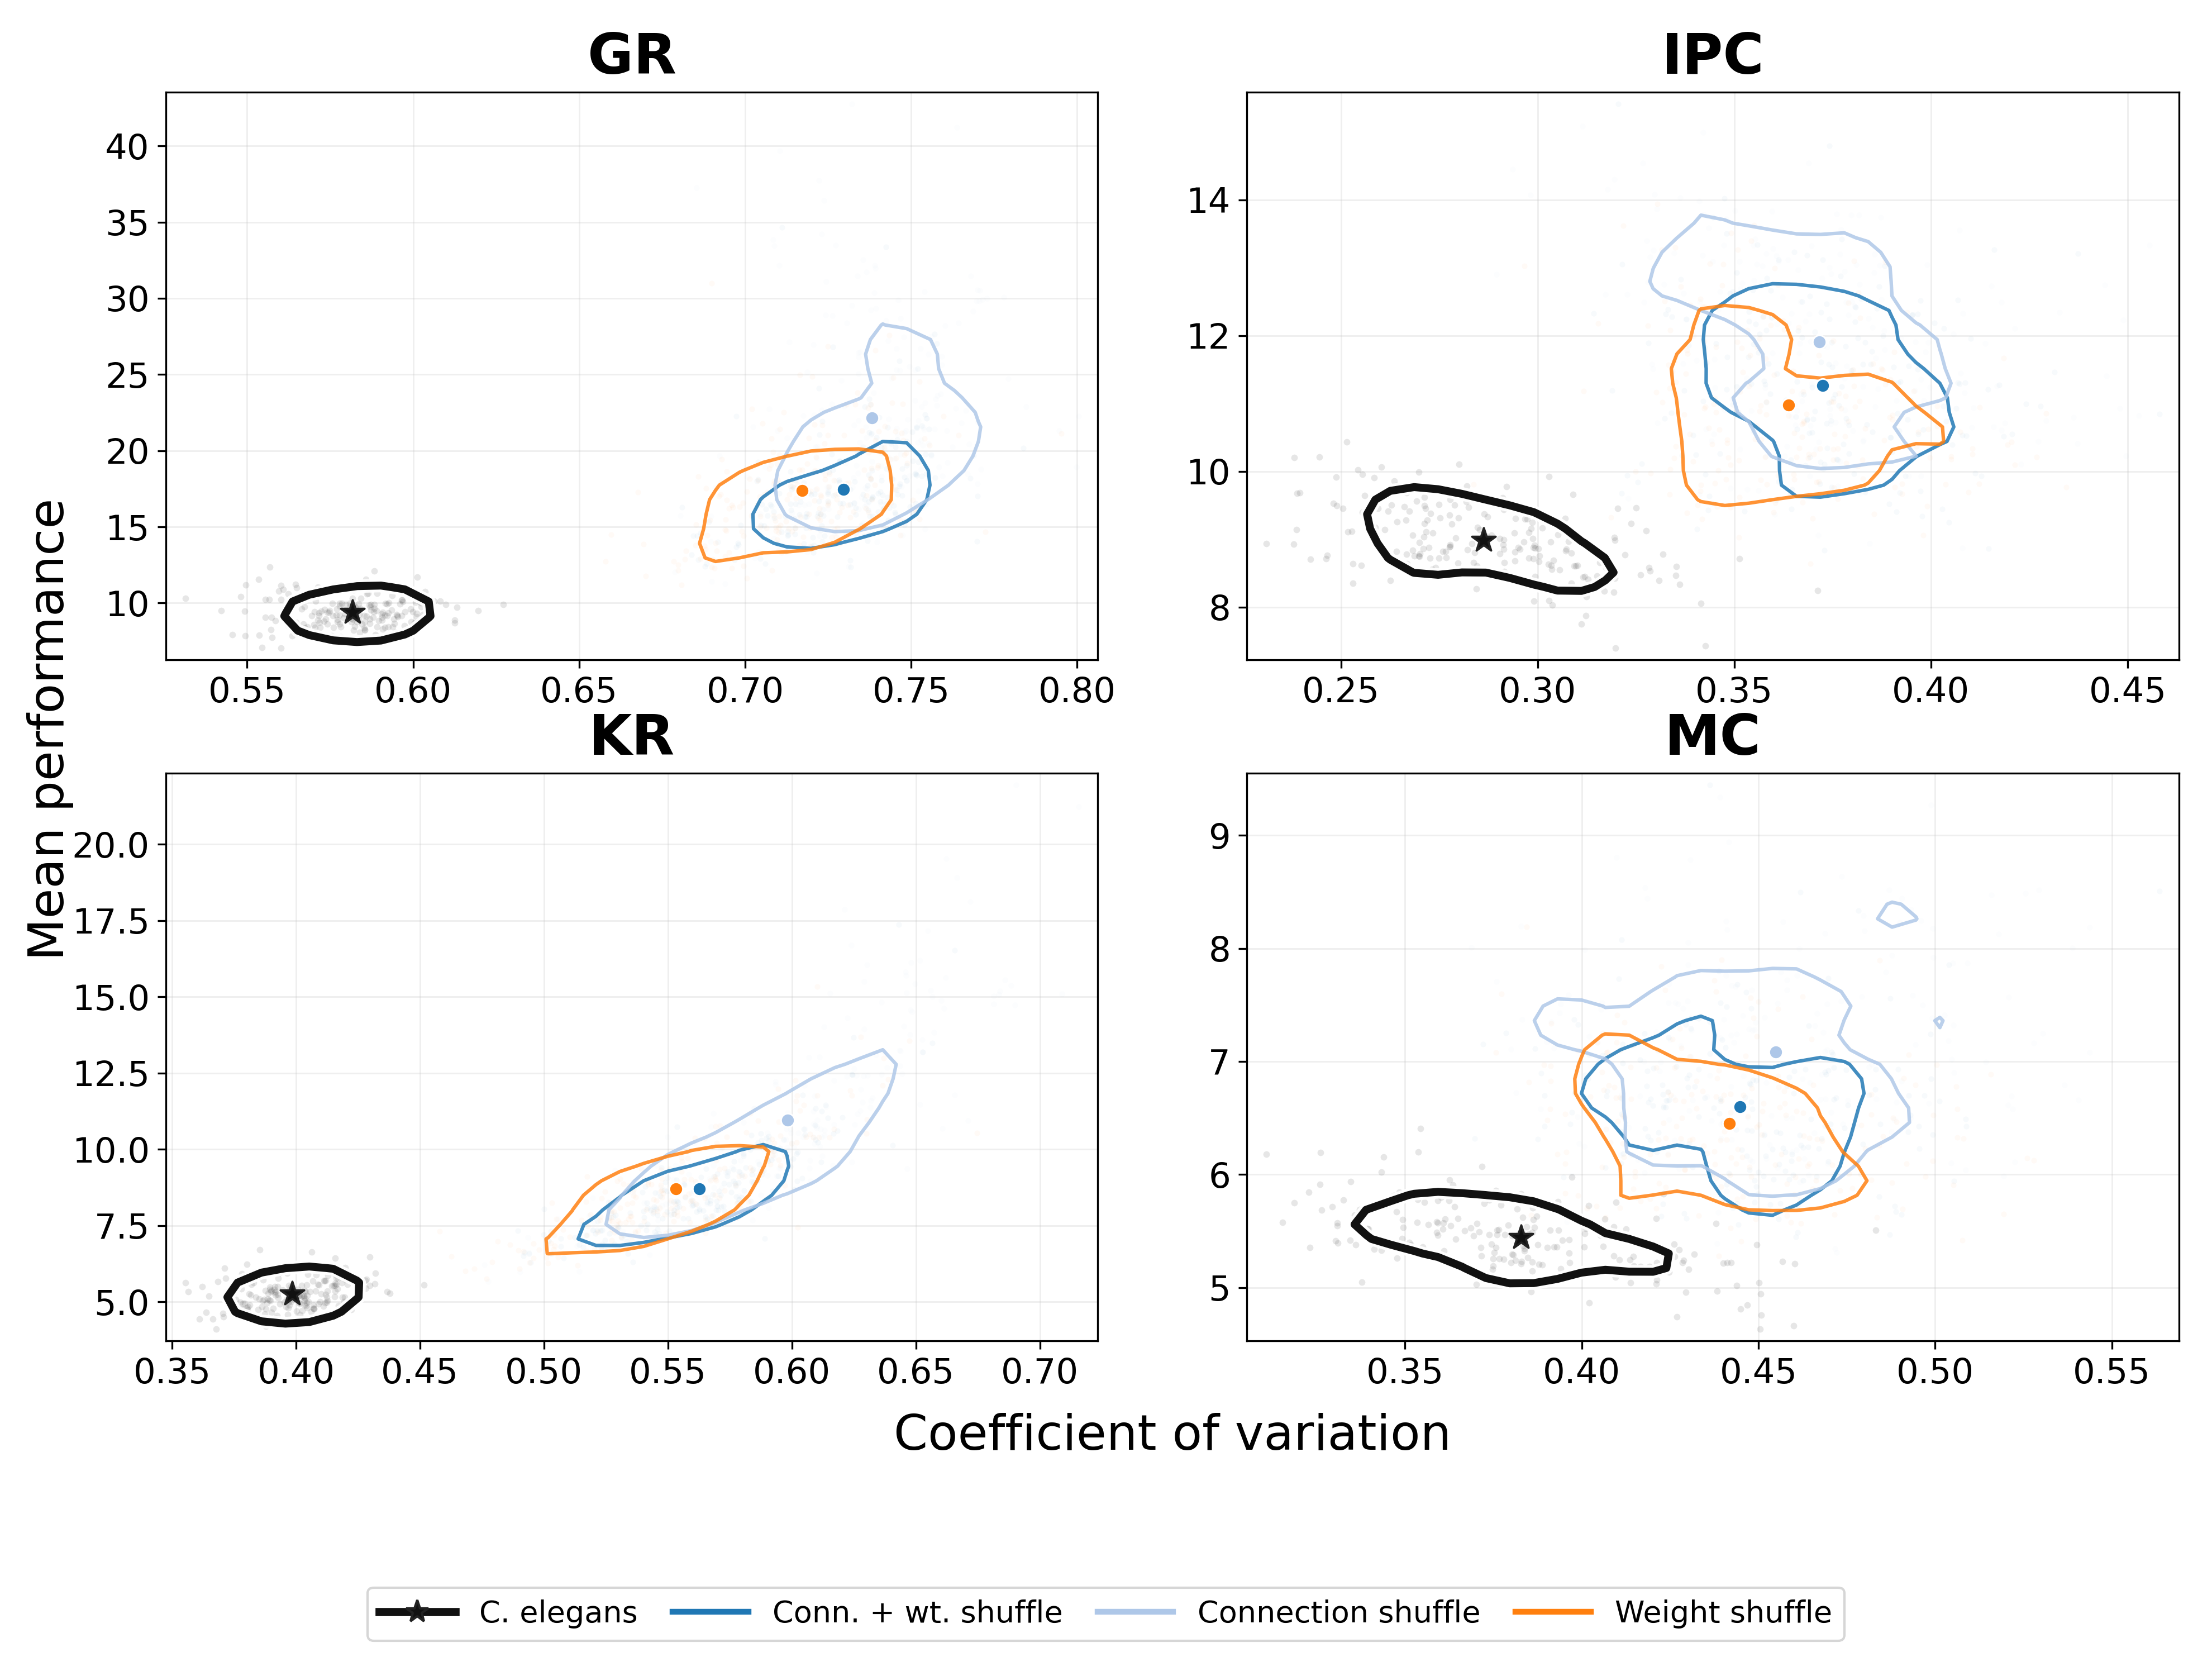
\includegraphics[width=\linewidth]{New_figs/shuf/real.png}
    \caption{
    Performance--CV islands for the original \textit{C.\ elegans} weight matrix and its shuffled variants, shown with 50\% density contours. Panels correspond to GR, IPC, KR, and MC. The black starred island marks the original connectome; blue marks connection-plus-weight shuffle; light blue marks connection shuffle; orange marks weight shuffle.}
    \label{fig:realW}
\end{figure}

\begin{figure}
    \centering
    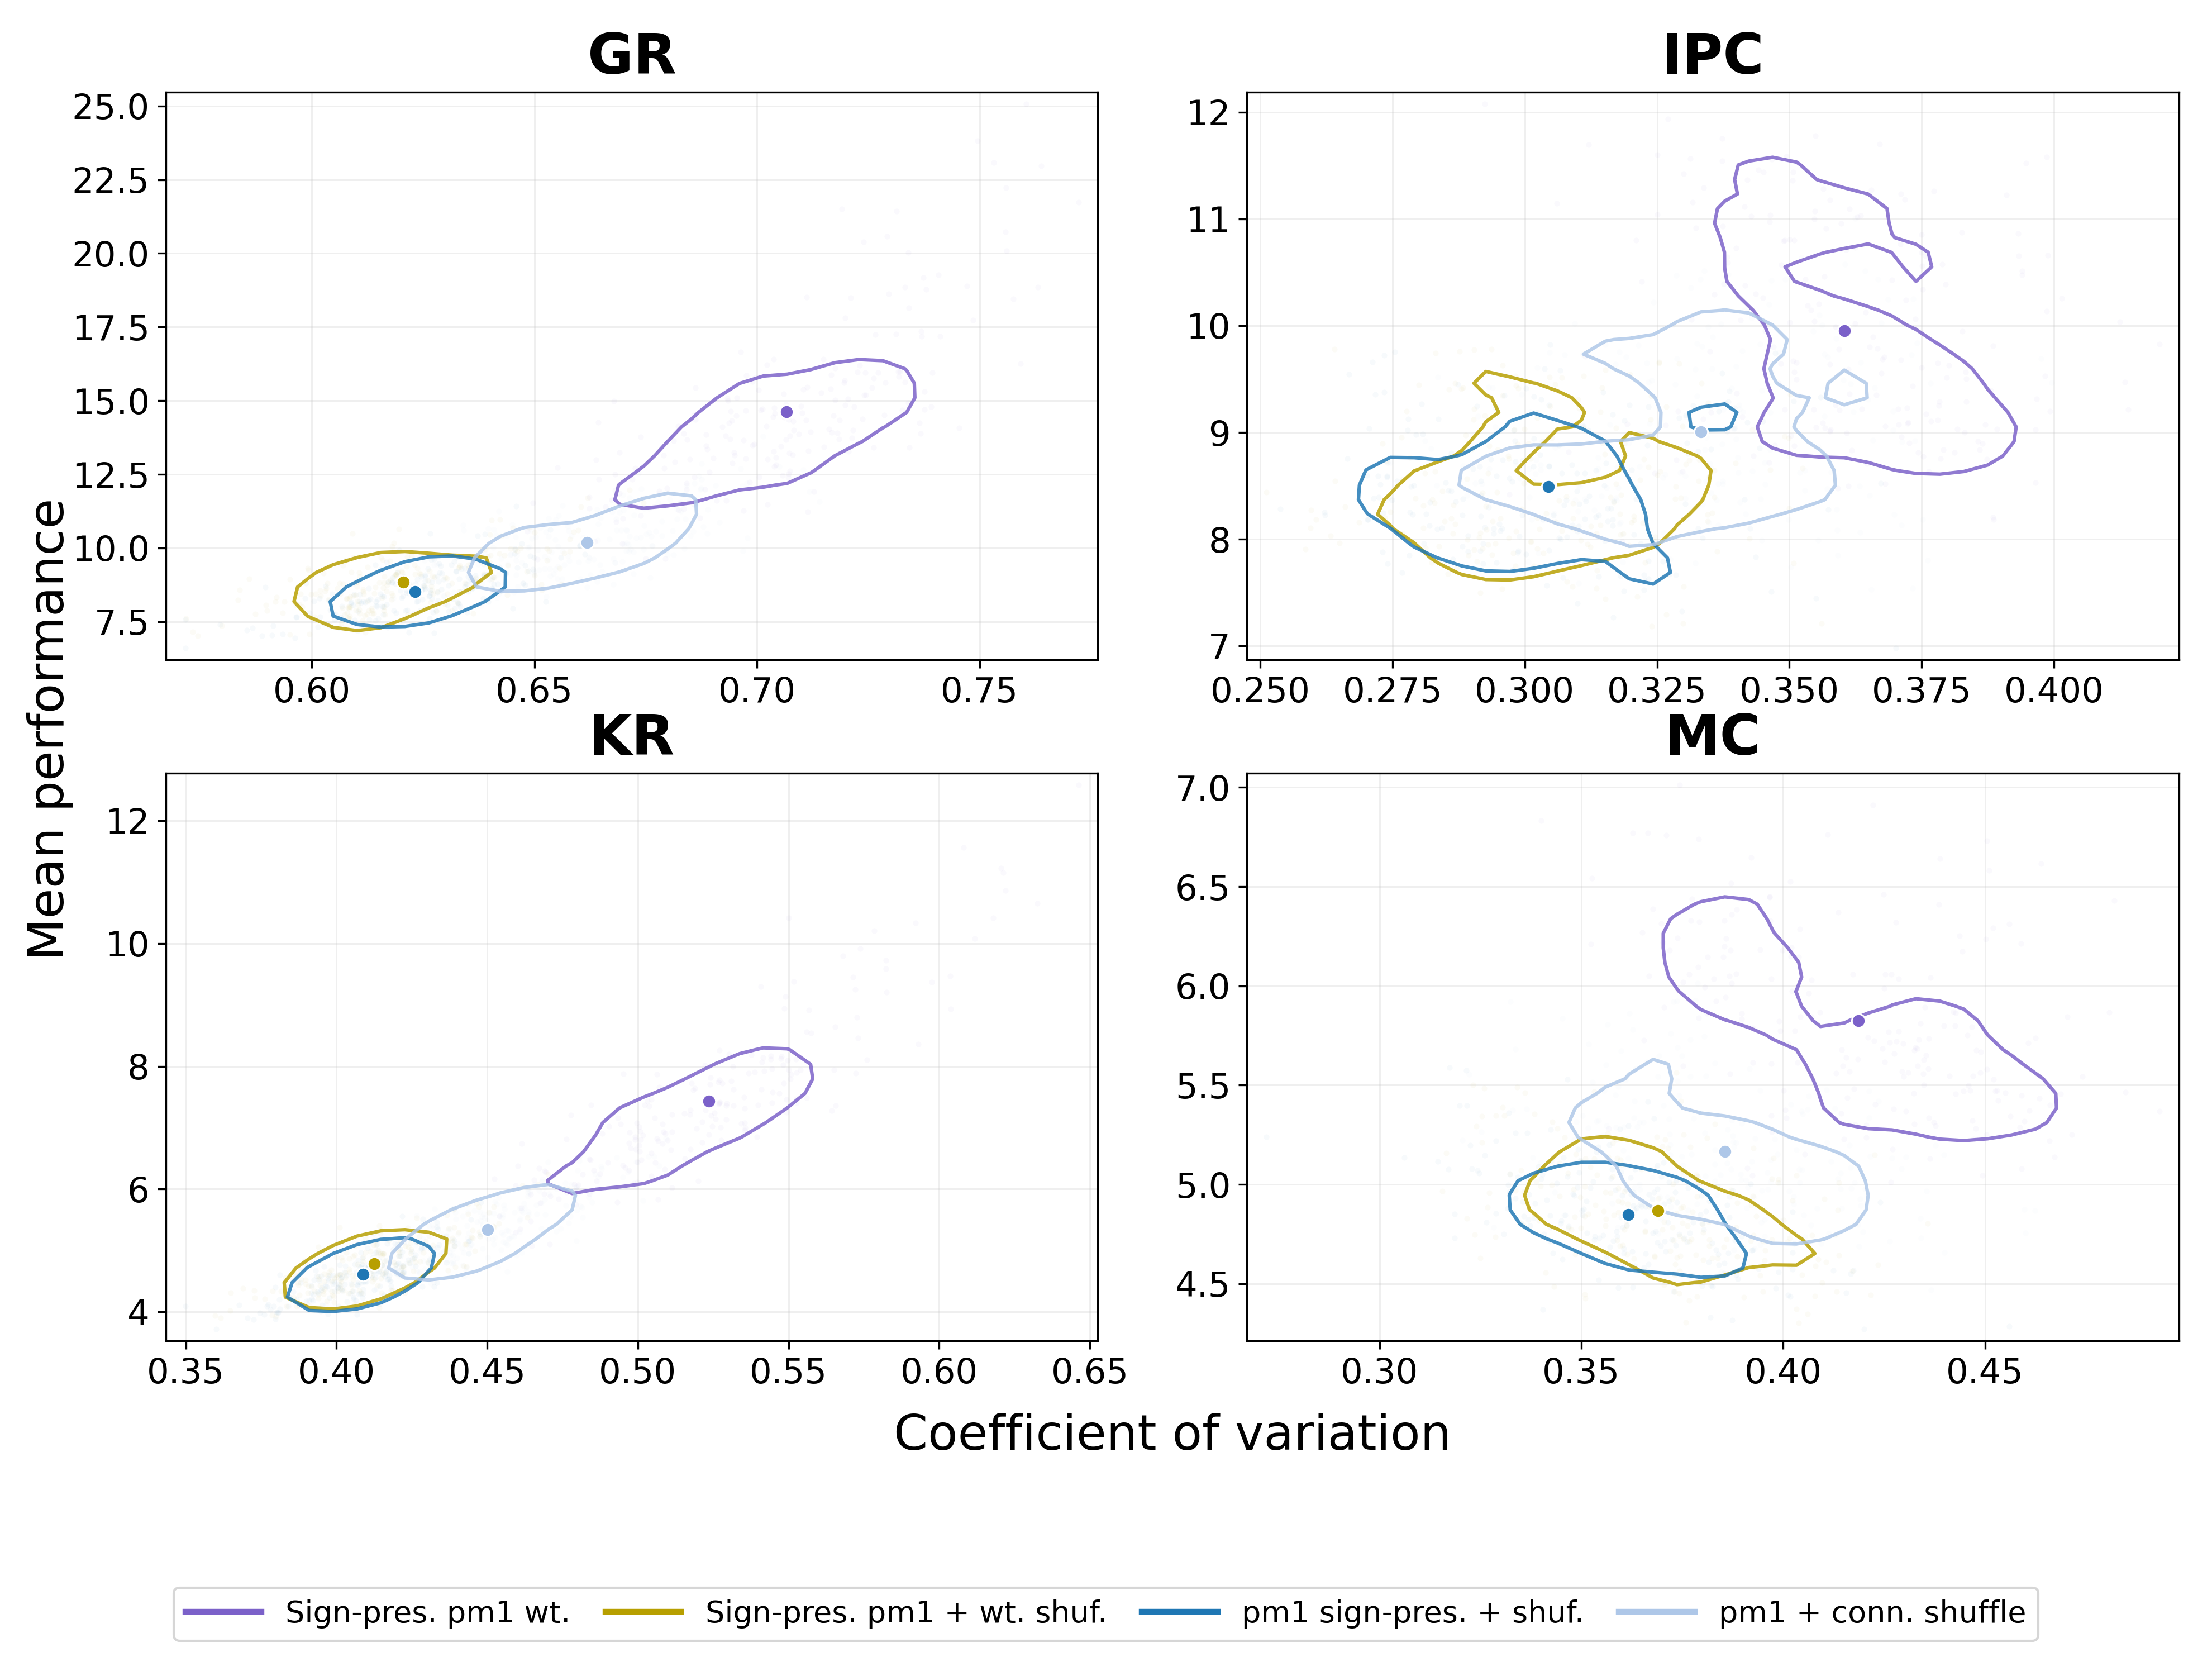
\includegraphics[width=\linewidth]{New_figs/shuf/pm1.png}
    \caption{
    Performance--CV islands for the \textit{C.\ elegans} topology with $\pm 1$ weights and its shuffled variants, shown with 50\% density contours. Panels correspond to GR, IPC, KR, and MC. The starred island marks the sign-preserving signed-unit baseline.}
    \label{fig:pm1W}
\end{figure}

\begin{figure}
    \centering
    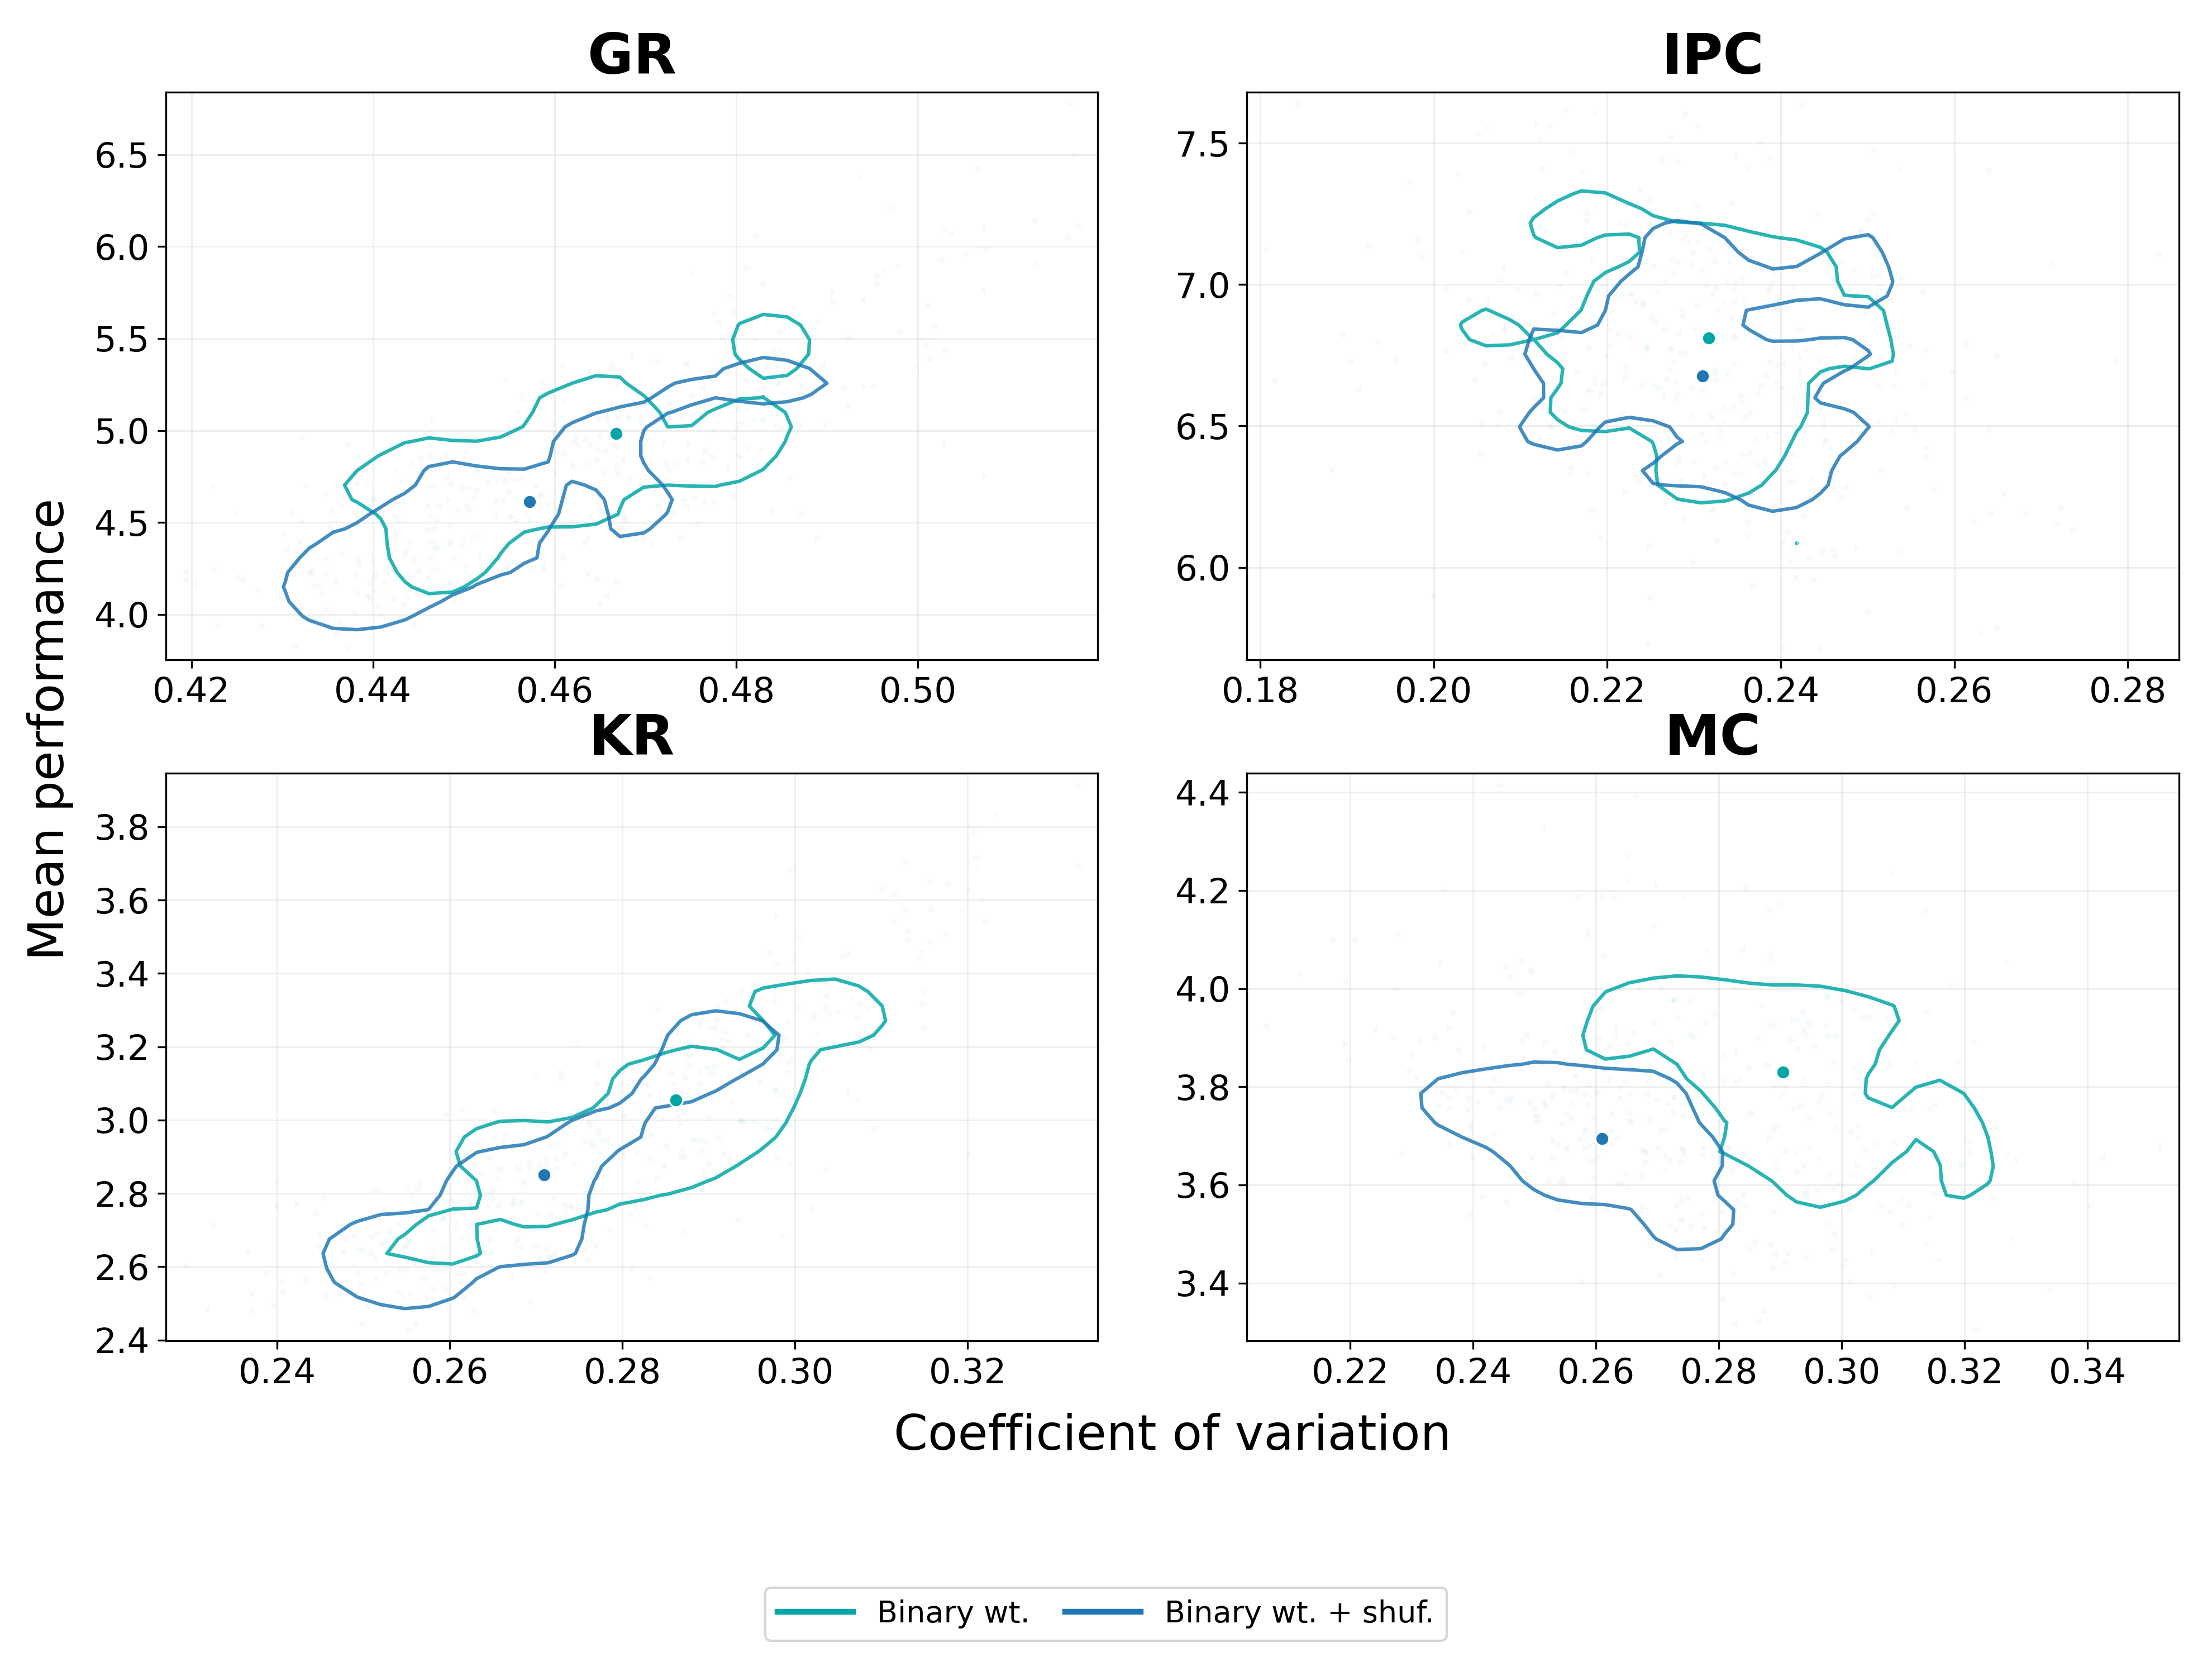
\includegraphics[width=\linewidth]{New_figs/shuf/binary_base.png}
    \caption{
    Performance--CV islands for the \textit{C.\ elegans} topology with binary weights and its degree-preserving connection-shuffled counterpart, shown with 50\% density contours. Panels correspond to GR, IPC, KR, and MC. Once every edge has the same positive sign and magnitude, residual shifts mainly reflect topology.}
    \label{fig:bW}
\end{figure}


\section{Discussion}
The central result of this manuscript is not that every structural feature contributes equally to hyperparameter invariance. The \textit{C.\ elegans} connectome occupies a relatively low-variance reservoir regime, and the ablations point to a conditional hierarchy of causes. Global E/I sign imbalance is the strongest single explanation in the model studied here: preserving the empirical sign ratio recovers much of the connectome's invariance for IPC, KR, and GR, even when exact sign placement and empirical weight magnitudes are simplified. This hierarchy is conditional because sign balance does not act in isolation. Its apparent explanatory power depends on the topology it is placed on, the distribution of weight magnitudes, the placement of those magnitudes, and the placement of inhibitory signs.

The sign-flipping experiments place this result in a performance--invariance tradeoff. Moving toward a more balanced E/I regime generally increases mean task-agnostic performance, but it also increases CV across spectral radius, leak rate, input scaling, and neuron bias. Under the present modeling choices, the empirical \textit{C.\ elegans} instantiation lies on the low-variance side of this curve rather than at the peak-performance region. Put more directly, the approximately 4:1 excitatory-to-inhibitory balance associated with many biological networks does not prioritize peak reservoir performance in this abstraction; it produces a more hyperparameter-invariant, lower-performance operating point. The result is therefore not a universal claim about E/I imbalance alone, but a statement about how this sign ratio acts in combination with the other structural choices in the present reservoir model.

The secondary effects are metric-specific. MC is the clearest architecture-level exception to the sign-balance account: it is not recovered by the sign-preserving $\pm 1$ controls and remains sensitive to topology and heterogeneous weights. The shuffle experiments support the same conclusion, but they also show that the residual structure is not restricted to MC. In the real-weight controls, connection shuffling and weight shuffling both move the reservoir toward higher-performance, higher-CV regimes, with the largest CV increases in KR. In the signed-unit controls, the original local sign placement has higher CV than the sign- and topology-shuffled controls despite a fixed global sign ratio. These effects are smaller than the global sign-balance sweep, but they are necessary for explaining where the empirical connectome sits within the performance--invariance tradeoff.

Magnitude effects become interpretable only after sign structure is fixed. Perturbing the empirical magnitude distribution toward a half-normal target has limited effect when signs and topology are preserved, so that experiment is best understood as a control against over-attributing the result to weight-distribution shape. By contrast, sign-preserving interpolation toward shuffled empirical magnitudes increases both mean performance and CV, especially for KR and GR. Magnitude placement therefore tunes the performance--invariance tradeoff within the sign-defined regime. It is not secondary in a universal sense; in this model it modulates, amplifies, or limits the effect of sign imbalance rather than replacing it as the largest observed driver for IPC, KR, and GR.

The no-strong-loops result also sharpens the interpretation of topology-sensitive residuals. In this study, MC is the metric least fully explained by global sign ratio in the architecture comparison and remains sensitive to topology and heterogeneous weights. KR is also strongly affected by several shuffle controls, especially real-weight connection shuffling. Hadaeghi et al. report the same kind of structural sensitivity from a different direction: increasing reciprocity changes the leading eigenvalue structure and lowers memory capacity, especially when the resulting increase in spectral radius forces stronger downscaling of recurrent weights during normalization \parencite{hadaeghi_no_strong_loops_2025}. This supports the conditional hierarchy proposed here. Global sign imbalance accounts for the largest IPC, KR, and GR invariance pattern within the tested models, while MC and KR retain stronger dependence on graph organization, loop structure, and the spectral constraints those structures impose.

Direct biological interpretation should be cautious because the connectome model compresses substantial uncertainty into a static signed network. The main analyses use EleganSign-derived signed connectomes, but many biological connections have unknown or complex sign annotations, and the inferred inhibitory fraction depends on how those ambiguous cases are handled \parencite{fenyves_szilágyi_zsolt_vassy_csaba_2020,elegansign_web}. We therefore analyze both a signed-only version that removes those ambiguous edges and an augmented version that assigns them random signs under a 4:1 excitatory-to-inhibitory prior. If the true inhibitory fraction differs from either approximation, the empirical connectome may lie elsewhere along the observed performance--CV curve. In addition, E/I balance varies across development and aging \parencite{wirak_florman_alkema_connor_gabel_2022, tanis_bellemer_moresco_forbush_koelle_2009}, and our model delivers inputs to all neurons rather than to biologically segregated populations. The present work should therefore be read as a structural reservoir analysis, not a faithful dynamical simulation of the animal.

For reservoir computing, the practical implication is that E/I sign ratio should be treated as an important design parameter for controlling the tradeoff between robustness and task-agnostic performance, complementing recent performance-focused work on adaptive E/I control in reservoirs \parencite{srinivasan_ei_balance_2025}. Its relative power should be evaluated alongside topology, sign placement, magnitude distribution, and magnitude placement rather than assumed in advance. In the present experiments, topology and heterogeneous weights matter strongly for MC and KR, while magnitude placement especially affects KR and GR after sign structure is fixed.

\subsection{Future directions}

Several extensions would help clarify these interpretations. First, the model comparisons could be strengthened by adding additional topology controls that match degree and sign statistics more tightly, including degree-matched random and scale-free networks. Such controls would help determine which residual effects are genuinely topological and whether the distinctive sensitivity of MC persists outside the \textit{C.\ elegans} degree distribution.

Second, the present conclusions should be tested on downstream tasks such as NARMA to determine whether the same structural relationships hold when reservoirs are evaluated by task performance rather than task-agnostic statistics alone. The same framework could also be used to investigate how connectome optimization algorithms \parencite{churchland_garcia-ojalvo_2026} alter task-agnostic statistics, and whether task-driven optimization moves biological reservoirs along the same performance--invariance axes identified here. Extending the ablation grid across additional topologies, magnitude distributions, and sign-placement rules would also test how far the relative importance of E/I imbalance generalizes beyond the present connectome-centered setting.

Third, it would be valuable to repeat these experiments with biologically segregated input and output populations. Using sensory neurons as inputs and muscles or motor neurons as outputs would bring the model closer to a functional circuit interpretation and would better connect this work to prior studies of connectome-based computation \parencite{KAWAI201915,yu_bpu_2025}. Finally, the role of sign inference deserves more direct study. Natural next steps would be to compare alternative neurotransmitter-to-sign mappings and to repeat the sign-balance analyses under inferred inhibitory fractions closer to those suggested by recent biological work.





\section*{AI Usage Disclosure}

Artificial intelligence tools, specifically ChatGPT (OpenAI, GPT-5 series) and Codex (OpenAI), were used as assistive tools during the course of this work.

AI tools were used to review text for clarity, grammar, and structure, and to identify ambiguous or overstated claims. All text included in this manuscript was written, reviewed, and edited by the authors, and any AI-assisted edits were manually verified and revised as necessary to ensure accuracy.

AI tools were also used to assist in identifying relevant literature. These tools were used in a search-assistance capacity to locate papers related to reservoir computing and recurrent biological networks. All cited papers were independently located, read, and verified by the author prior to inclusion.

In addition, AI tools were used as a programming reference to identify relevant libraries, functions, and debugging strategies. They were also used to assist in generating example plotting code and suggesting implementation approaches. All code used in this project was written, reviewed, and validated by the author.

AI tools were used solely as assistive instruments. All scientific claims, analysis, interpretations, and conclusions presented in this work are the independent work of the author.


\appendix
\section{Supplemental Information}


\subsection{Architecture details}
\label{supp:architectures}
This section gives the full architecture definitions summarized in Table~\ref{tab:architecture_groups}. The quantitative analyses use the EleganSign-derived preprocessing versions described in Section~\ref{sec:connectome_dataset}: a 297-node, 1740-edge signed-only graph and an augmented random-sign graph that retains the 1864 unknown or complex-sign edges under a 4:1 excitatory-to-inhibitory prior. The visualization panels in this supplemental section were generated from the earlier c302-derived connectome and are retained only as schematic illustrations of the control families.

\begin{figure}[t]
    \centering
    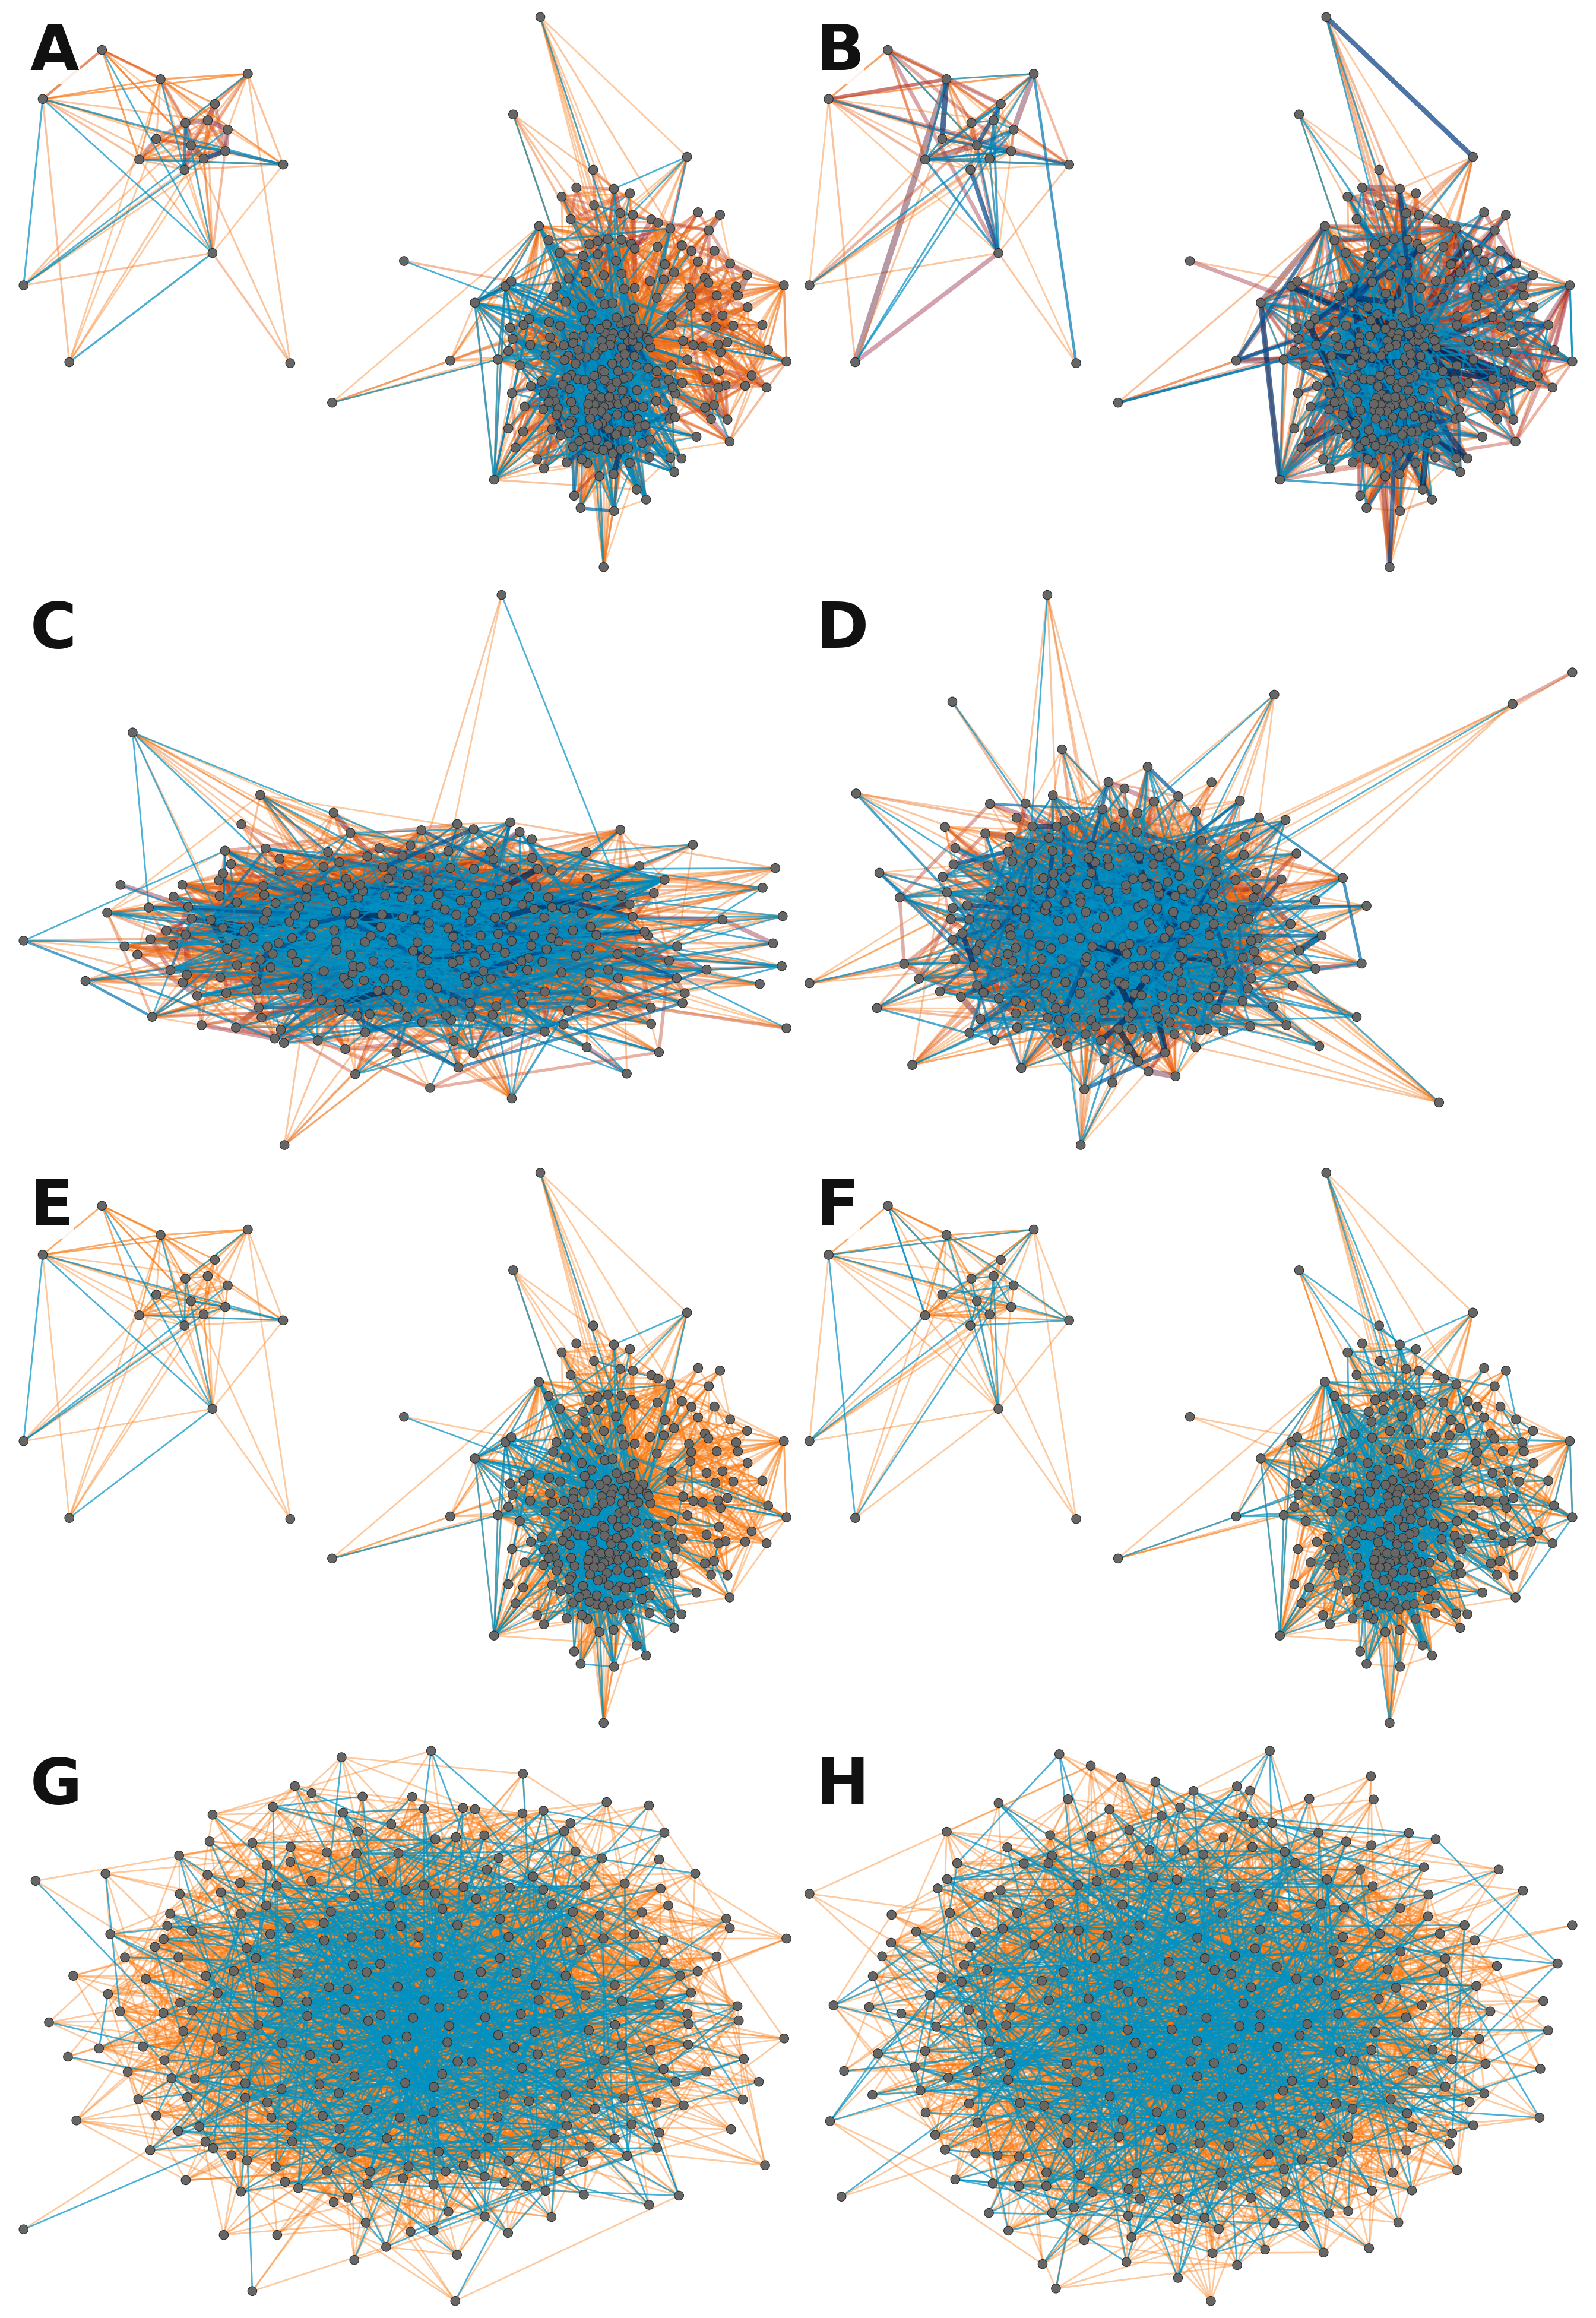
\includegraphics[width=0.75\textwidth]{figs/toplogy/model_grid_A_to_H.png}
    \caption{Network visualizations for architectures A--H. In all panels, nodes represent neurons, orange edges are excitatory synapses, blue edges are inhibitory synapses, and darker edges indicate stronger synaptic weights. A: original \emph{C.~elegans} connectome. B: original connectome with shuffled weights. C: connection-shuffled \emph{C.~elegans} connectome. D: connection-shuffled connectome with an additional weight shuffle. E: original topology with signed binary ($\pm 1$) weights determined by the original edge signs. F: panel E after sign shuffling. G: connection-shuffled version of panel E. H: panel G after sign shuffling.}
\end{figure}

\begin{figure}[t]
    \centering
    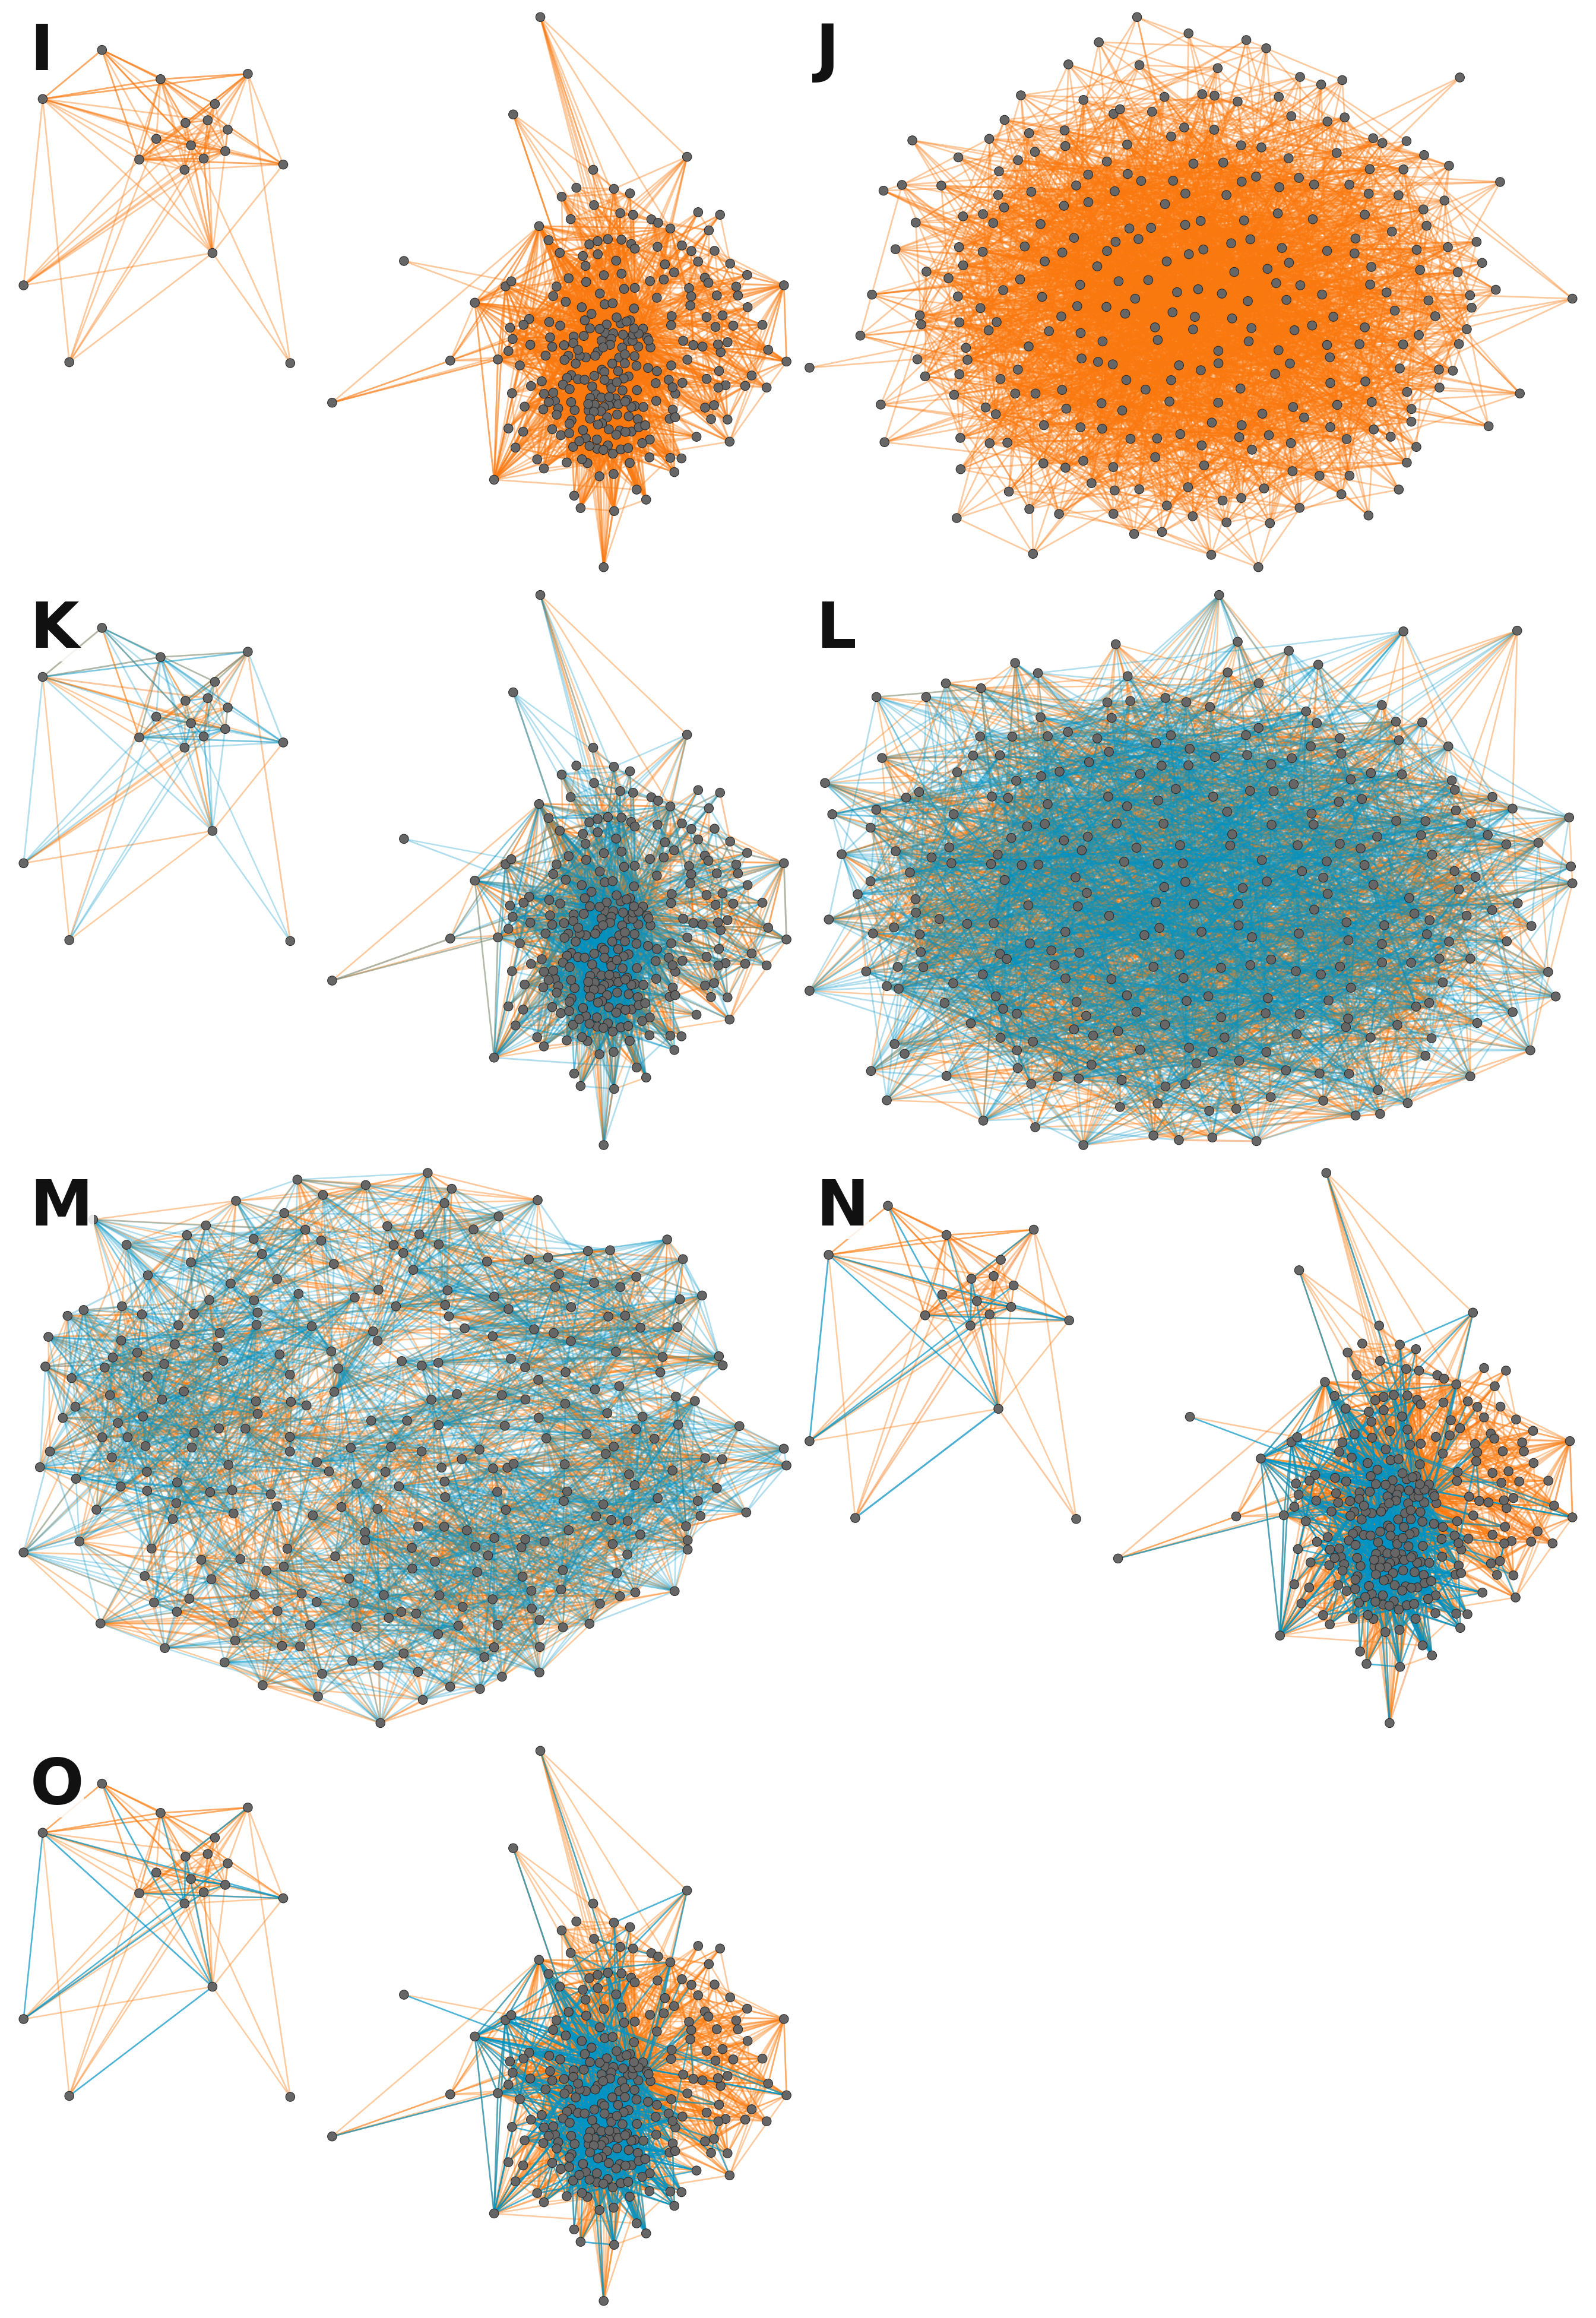
\includegraphics[width=0.75\textwidth]{figs/toplogy/model_grid_I_to_O.png}
    \caption{Additional control architectures I--O. I: \emph{C.~elegans} connectome with binary weights. J: binary-weight \emph{C.~elegans} connectome after connection shuffling. K: \emph{C.~elegans} topology with Gaussian weights. L: \emph{C.~elegans}-matched Erd\H{o}s--R\'enyi network with Gaussian weights. M: small-world network with $p = 0.1$ and Gaussian weights. N: sign-preserving Gaussian model. O: sign-preserving uniform model.}
\end{figure}

\subsubsection{C. elegans connectome}
This uses the biological network and contact-count weights:
\[
W_{ij}=W^{cel}_{ij}.
\]

\subsubsection{Original \textit{C.\ elegans} connectome with weight shuffle}
\label{sec:original_weight_shuffle}
Starting from the original \textit{C.\ elegans} connectome, this architecture preserves biological topology but shuffles the weights across existing connections using the weight-shuffle procedure in Section~\ref{Weight-Shuffle}.

\subsubsection{Original \textit{C.\ elegans} connectome with connection shuffle}
\label{sec:original_connection_shuffle}
Starting from the original \textit{C.\ elegans} connectome, this architecture applies the degree-preserving connection-shuffle procedure in Section~\ref{Connection-Shuffle}.

\subsubsection{Connection shuffle with weight shuffle}
The \textit{C.\ elegans} connectome is first connection-shuffled as described in Section~\ref{Connection-Shuffle}, and the resulting nonzero weights are then shuffled as described in Section~\ref{Weight-Shuffle}.

\subsubsection[C. elegans architecture with signed unit weights using original connection signs]{C. elegans architecture with $\pm 1$ weights using original connection signs}
\label{sec:plus1minus1network}
This architecture preserves the biological topology and edge signs while setting every nonzero magnitude to one:
\[
W_{ij}' =
\begin{cases}
\operatorname{sign}(W_{ij}) & \text{if } W_{ij} \neq 0,\\
0 & \text{if } W_{ij} = 0.
\end{cases}
\]

\subsubsection[C. elegans architecture with signed unit weights and shuffled signs preserving sign balance]{C. elegans architecture with $\pm 1$ weights and shuffled signs preserving sign balance}
This control keeps the biological connectivity fixed but randomizes which edges carry inhibitory signs. If
\[
N_-=\#\{(i,j):W'_{ij}=-1\},
\]
then a random subset of size \(N_-\) of nonzero entries is assigned sign \(-1\), and all remaining nonzero entries are assigned sign \(+1\). This preserves the global E/I sign ratio while shuffling sign placement.

\subsubsection[C. elegans architecture with signed unit weights under connection shuffling]{C. elegans architecture with $\pm 1$ weights under connection shuffling}
Starting from the signed unit-magnitude network in Section~\ref{sec:plus1minus1network}, the edge set is connection-shuffled as described in Section~\ref{Connection-Shuffle}.

\subsubsection[C. elegans architecture with signed unit weights under connection and weight shuffling]{C. elegans architecture with $\pm 1$ weights under connection shuffling and weight shuffling}
Starting from the signed unit-magnitude network in Section~\ref{sec:plus1minus1network}, the edge set is connection-shuffled and then the signed unit weights are shuffled across the resulting nonzero entries.

\subsubsection{C. elegans architecture with binary weights}
This ablation preserves the biological connectivity pattern but removes both sign and magnitude heterogeneity:
\[
W_{ij}' =
\begin{cases}
1 & \text{if } W_{ij} \neq 0,\\
0 & \text{if } W_{ij} = 0.
\end{cases}
\]

\subsubsection{C. elegans architecture with binary weights and connection shuffle}
This binary network is rewired with the procedure in Section~\ref{Connection-Shuffle}.

\subsubsection{C.~elegans topology with Gaussian weights}
This control keeps the biological connectivity pattern but replaces each nonzero weight with an independent Gaussian sample:
\[
W'_{ij} =
\begin{cases}
X_{ij} & \text{if } W_{ij} \neq 0,\\
0 & \text{if } W_{ij} = 0,
\end{cases}
\qquad
X_{ij}\sim\mathcal{N}(0,1).
\]

\subsubsection{C.~elegans--matched Erd\H{o}s--R\'enyi model with Gaussian weights}
This random-graph baseline uses \(N=297\) nodes and an adjusted ER edge set with the same number of directed edges as the analysis \emph{C.~elegans} network. After fixing the edge count, weights are independently sampled from \(\mathcal{N}(0,1)\).

\subsubsection{Watts--Strogatz Gaussian control}
This small-world control uses \(N=297\) nodes and \(1740\) directed edges. A directed ring lattice is rewired with probability \(p=0.1\), preserving source out-degree and edge count, and nonzero weights are independently sampled from \(\mathcal{N}(0,1)\).

\subsubsection{C. elegans architecture with half Gaussian weights using original connection signs}
Starting from the signed unit-magnitude network in Section~\ref{sec:plus1minus1network}, magnitudes are sampled from a half-Gaussian distribution:
\[
W_{ij}'=\operatorname{sign}(W_{ij})|\mathcal{N}(0,1)|.
\]

\subsubsection{C. elegans architecture with uniform weights using original connection signs}
Starting from the signed unit-magnitude network in Section~\ref{sec:plus1minus1network}, magnitudes are sampled independently from a uniform distribution:
\[
W_{ij}'=\operatorname{sign}(W_{ij})X_{ij},
\qquad
X_{ij}\sim\mathcal{U}(0,1).
\]

\subsection{Shuffle experiment CV summaries}
\label{supp:shuffle_cv}
Tables~\ref{tab:shuffle_cv_real}--\ref{tab:shuffle_cv_binary} report the paired changes in mean hyperparameter CV for the shuffle experiments shown in Figure~\ref{fig:realW}, Figure~\ref{fig:pm1W}, and Figure~\ref{fig:bW}. Positive values indicate higher CV than the corresponding baseline, and negative values indicate lower CV. Each comparison uses \(n=200\) paired trial groups.

\begin{table}[p]
    \centering
    \scriptsize
    \caption[Mean CV differences for real-valued shuffle controls]{Mean CV differences for real-valued shuffle controls relative to the empirical \textit{C.\ elegans} reservoir. Baseline CV and control CV are mean coefficients of variation across the 96-point hyperparameter sweep. \(\Delta\)CV is control minus baseline.}
    \label{tab:shuffle_cv_real}
    \resizebox{\textwidth}{!}{\begin{tabular}{llrrrr}
\toprule
Metric & Control & C. elegans mean CV & Control mean CV & $\Delta$CV & $\Delta$CV (\%) \\
\midrule
MC & Conn. + wt. shuffle & 0.3829 & 0.4448 & +0.0620 & +16.18 \\
MC & Connection shuffle & 0.3829 & 0.4549 & +0.0721 & +18.82 \\
MC & Weight shuffle & 0.3829 & 0.4418 & +0.0589 & +15.39 \\
IPC & Conn. + wt. shuffle & 0.2863 & 0.3724 & +0.0861 & +30.07 \\
IPC & Connection shuffle & 0.2863 & 0.3717 & +0.0853 & +29.80 \\
IPC & Weight shuffle & 0.2863 & 0.3638 & +0.0775 & +27.06 \\
KR & Conn. + wt. shuffle & 0.3985 & 0.5626 & +0.1641 & +41.17 \\
KR & Connection shuffle & 0.3985 & 0.5982 & +0.1997 & +50.11 \\
KR & Weight shuffle & 0.3985 & 0.5532 & +0.1547 & +38.80 \\
GR & Conn. + wt. shuffle & 0.5817 & 0.7296 & +0.1479 & +25.42 \\
GR & Connection shuffle & 0.5817 & 0.7381 & +0.1564 & +26.89 \\
GR & Weight shuffle & 0.5817 & 0.7172 & +0.1354 & +23.28 \\
\bottomrule
\end{tabular}
% Differences are control minus C. elegans; paired by trial where available.
}
\end{table}

\begin{table}[p]
    \centering
    \scriptsize
    \caption[Mean CV differences for signed-unit shuffle controls]{Mean CV differences for signed-unit shuffle controls relative to the original local sign-preserving signed-unit reservoir. Baseline CV and control CV are mean coefficients of variation across the 96-point hyperparameter sweep. \(\Delta\)CV is control minus baseline.}
    \label{tab:shuffle_cv_pm1}
    \resizebox{\textwidth}{!}{\begin{tabular}{llrrrrl}
\toprule
Metric & Control & Sign-pres. pm1 wt. mean CV & Control mean CV & $\Delta$CV & $\Delta$CV (\%) & 95\% CI \\
\midrule
MC & Sign-pres. pm1 + wt. shuf. & 0.4186 & 0.3690 & -0.0496 & -11.84 & [-0.0534, -0.0457] \\
MC & pm1 + conn. shuffle & 0.4186 & 0.3855 & -0.0331 & -7.90 & [-0.0367, -0.0295] \\
MC & pm1 sign-pres. + shuf. & 0.4186 & 0.3617 & -0.0569 & -13.59 & [-0.0608, -0.0530] \\
IPC & Sign-pres. pm1 + wt. shuf. & 0.3604 & 0.3047 & -0.0557 & -15.46 & [-0.0598, -0.0516] \\
IPC & pm1 + conn. shuffle & 0.3604 & 0.3332 & -0.0272 & -7.54 & [-0.0313, -0.0230] \\
IPC & pm1 sign-pres. + shuf. & 0.3604 & 0.3045 & -0.0559 & -15.51 & [-0.0597, -0.0521] \\
KR & Sign-pres. pm1 + wt. shuf. & 0.5236 & 0.4126 & -0.1110 & -21.20 & [-0.1168, -0.1052] \\
KR & pm1 + conn. shuffle & 0.5236 & 0.4501 & -0.0735 & -14.04 & [-0.0797, -0.0673] \\
KR & pm1 sign-pres. + shuf. & 0.5236 & 0.4088 & -0.1148 & -21.92 & [-0.1209, -0.1086] \\
GR & Sign-pres. pm1 + wt. shuf. & 0.7066 & 0.6205 & -0.0860 & -12.18 & [-0.0900, -0.0820] \\
GR & pm1 + conn. shuffle & 0.7066 & 0.6618 & -0.0448 & -6.34 & [-0.0490, -0.0406] \\
GR & pm1 sign-pres. + shuf. & 0.7066 & 0.6232 & -0.0833 & -11.79 & [-0.0876, -0.0790] \\
\bottomrule
\end{tabular}
% Differences are control minus Sign-pres. pm1 wt.; paired by trial where available.
}
\end{table}

\begin{table}[p]
    \centering
    \scriptsize
    \caption[Mean CV differences for the all-positive binary topology shuffle]{Mean CV differences for the all-positive binary topology shuffle relative to the all-positive binary \textit{C.\ elegans} topology. Baseline CV and control CV are mean coefficients of variation across the 96-point hyperparameter sweep. \(\Delta\)CV is control minus baseline.}
    \label{tab:shuffle_cv_binary}
    \resizebox{\textwidth}{!}{\begin{tabular}{llrrrrl}
\toprule
Metric & Control & Binary wt. mean CV & Control mean CV & $\Delta$CV & $\Delta$CV (\%) & 95\% CI \\
\midrule
MC & Binary wt. + shuf. & 0.2905 & 0.2610 & -0.0295 & -10.16 & [-0.0321, -0.0269] \\
IPC & Binary wt. + shuf. & 0.2317 & 0.2310 & -0.0007 & -0.30 & [-0.0035, +0.0021] \\
KR & Binary wt. + shuf. & 0.2862 & 0.2709 & -0.0153 & -5.34 & [-0.0176, -0.0130] \\
GR & Binary wt. + shuf. & 0.4668 & 0.4572 & -0.0095 & -2.04 & [-0.0117, -0.0074] \\
\bottomrule
\end{tabular}
% Differences are control minus Binary wt.; paired by trial where available.
}
\end{table}


\subsection{Weight and magnitude ablation controls}
\label{sec:magnitude_interpolation}
\label{sec:weight_perturbation}
The main results show that sign structure must be fixed before magnitude effects can be interpreted cleanly. The sign-preserving interpolation experiments therefore ask a narrower question: once topology and edge signs are held constant, does the placement of empirical magnitudes across signed edges matter?

Interpolating from signed unit magnitudes to the empirical \textit{C.\ elegans} magnitudes produces only modest changes (Figure~\ref{fig:bin_to_cel_interp}). At \(f=1\), CV changes by \(+7.39\%\) for MC, \(-0.635\%\) for IPC, \(+0.929\%\) for KR, and \(+0.775\%\) for GR. Mean metric values also change modestly. Thus, adding empirical magnitudes in their original locations does not substantially disrupt the low-variance regime once the empirical sign structure is already fixed.

The shuffled-magnitude interpolations behave differently. Moving from signed unit magnitudes to shuffled empirical magnitudes increases CV by \(17.5\%\) for MC, \(14.3\%\) for IPC, \(32.1\%\) for KR, and \(24.4\%\) for GR at \(f=1\) (Figure~\ref{fig:bin_to_cel_shuf_interp}). Directly interpolating from empirical magnitudes to shuffled empirical magnitudes produces a similar pattern, with especially large effects for KR and GR (Figure~\ref{fig:cel_to_cel_shuf_interp}). Because signs are preserved throughout these sweeps, the increase in CV cannot be attributed to altered E/I balance. It reflects the placement of heterogeneous magnitudes on the fixed signed topology.

The half-normal perturbation is best interpreted as a control rather than a main discovery. When connectivity and signs are preserved, moving the magnitude distribution toward a fitted shifted half-normal target produces only modest changes in both mean metric value and CV (Figure~\ref{fig:weights}). When sign is not preserved in the corresponding control, the changes are much larger. This confirms the ordering of causes: large effects attributed to magnitude perturbation can be dominated by sign-balance changes unless sign structure is explicitly fixed.

Together, the magnitude experiments complete the conditional hierarchy. Magnitude placement can move the reservoir toward higher mean performance and higher CV, particularly for KR and GR, but this effect appears after the sign structure has already set the main performance--invariance regime in these experiments. Empirical \textit{C.\ elegans} magnitudes are therefore not irrelevant; they tune metric-specific behavior within a regime strongly shaped by global E/I sign imbalance.

\begin{figure}
    \centering
    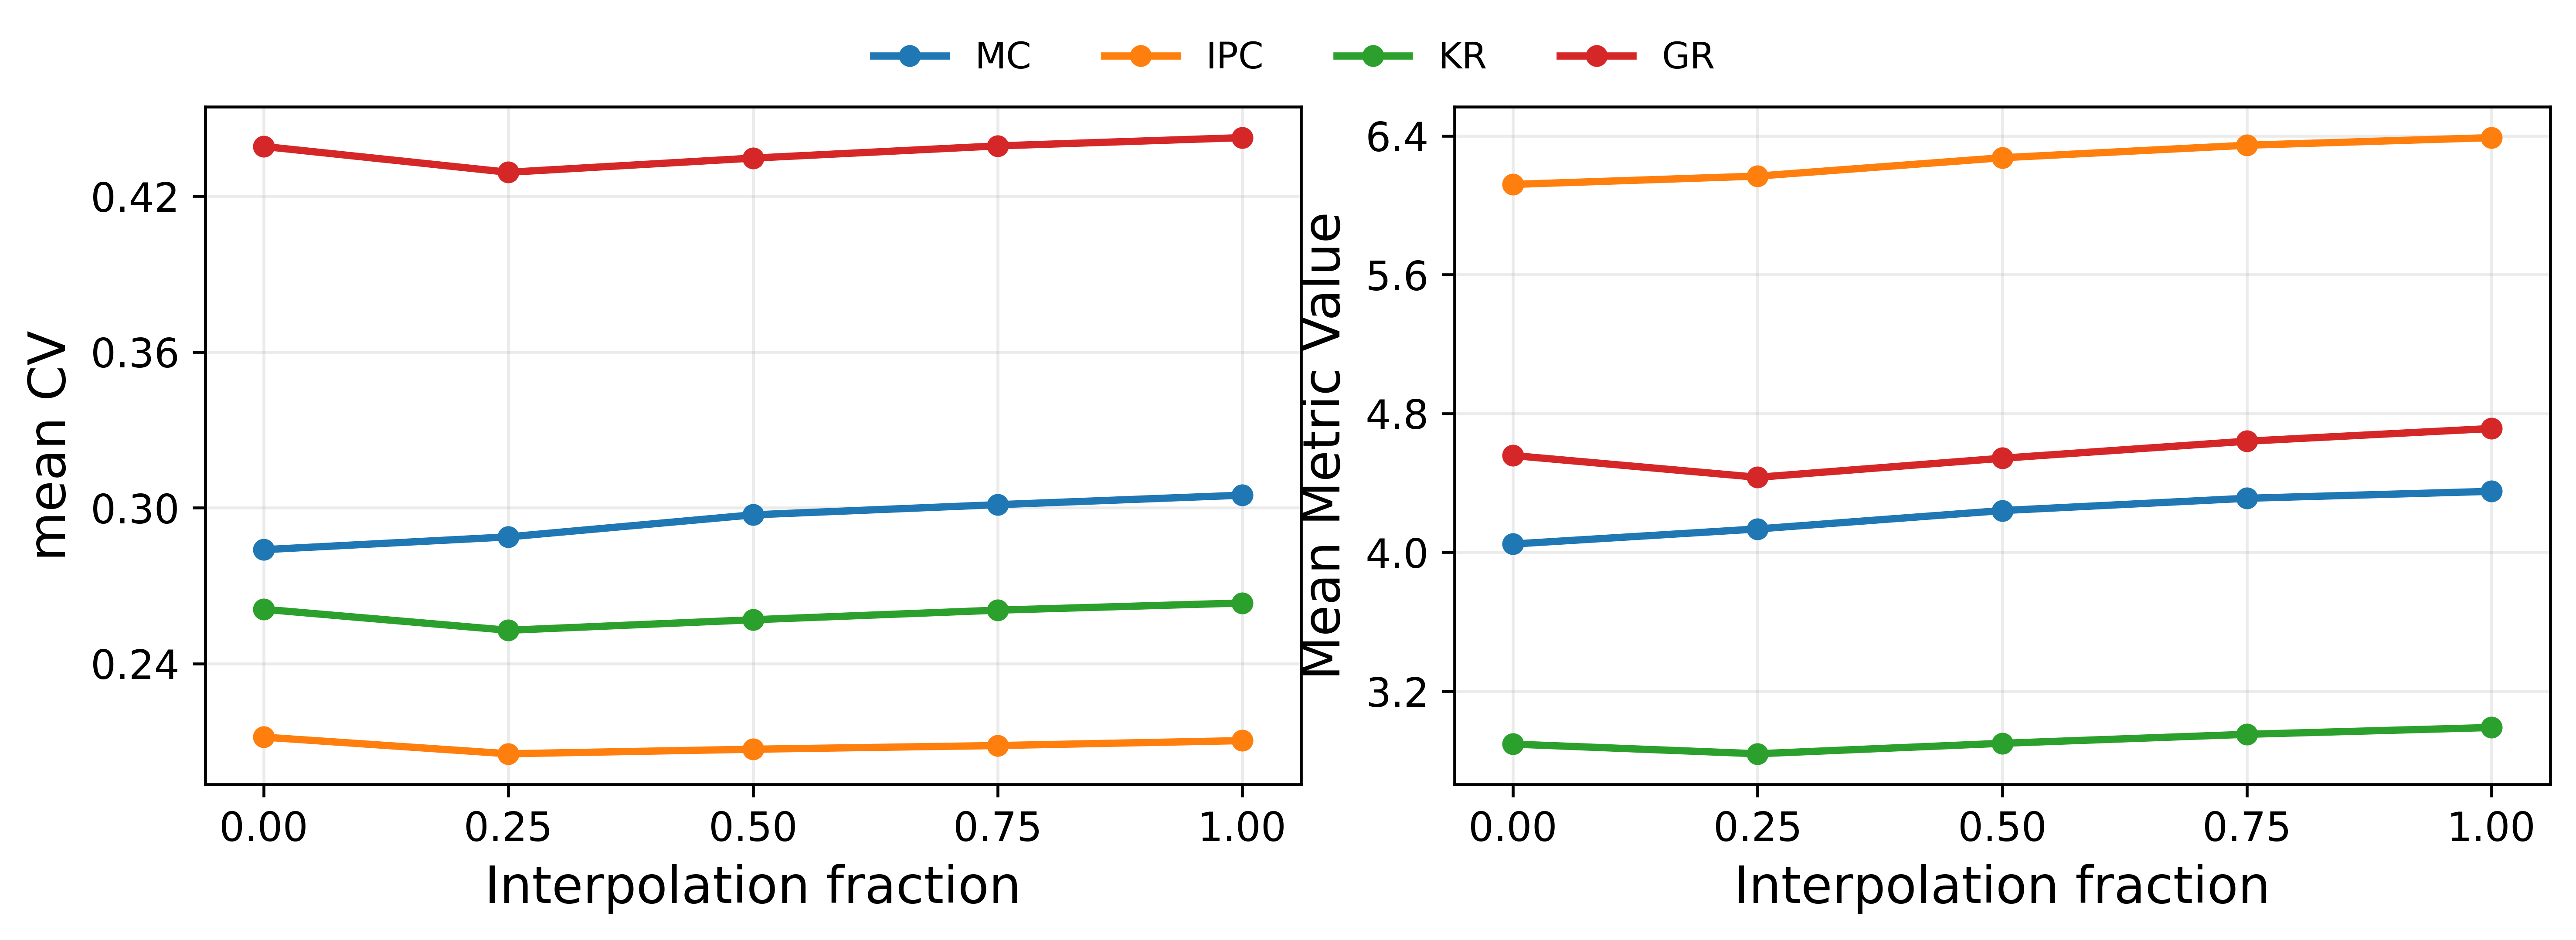
\includegraphics[width=\linewidth]{figs/interpolation/bin_to_cel.png}
    \caption{Sign-preserving interpolation from signed unit magnitudes to empirical \textit{C.\ elegans} magnitudes. The original topology and edge signs are fixed for every interpolation fraction; only nonzero magnitudes change. Left: mean CV across the hyperparameter sweep. Right: mean task-agnostic metric value.}
    \label{fig:bin_to_cel_interp}
\end{figure}

\begin{figure}
    \centering
    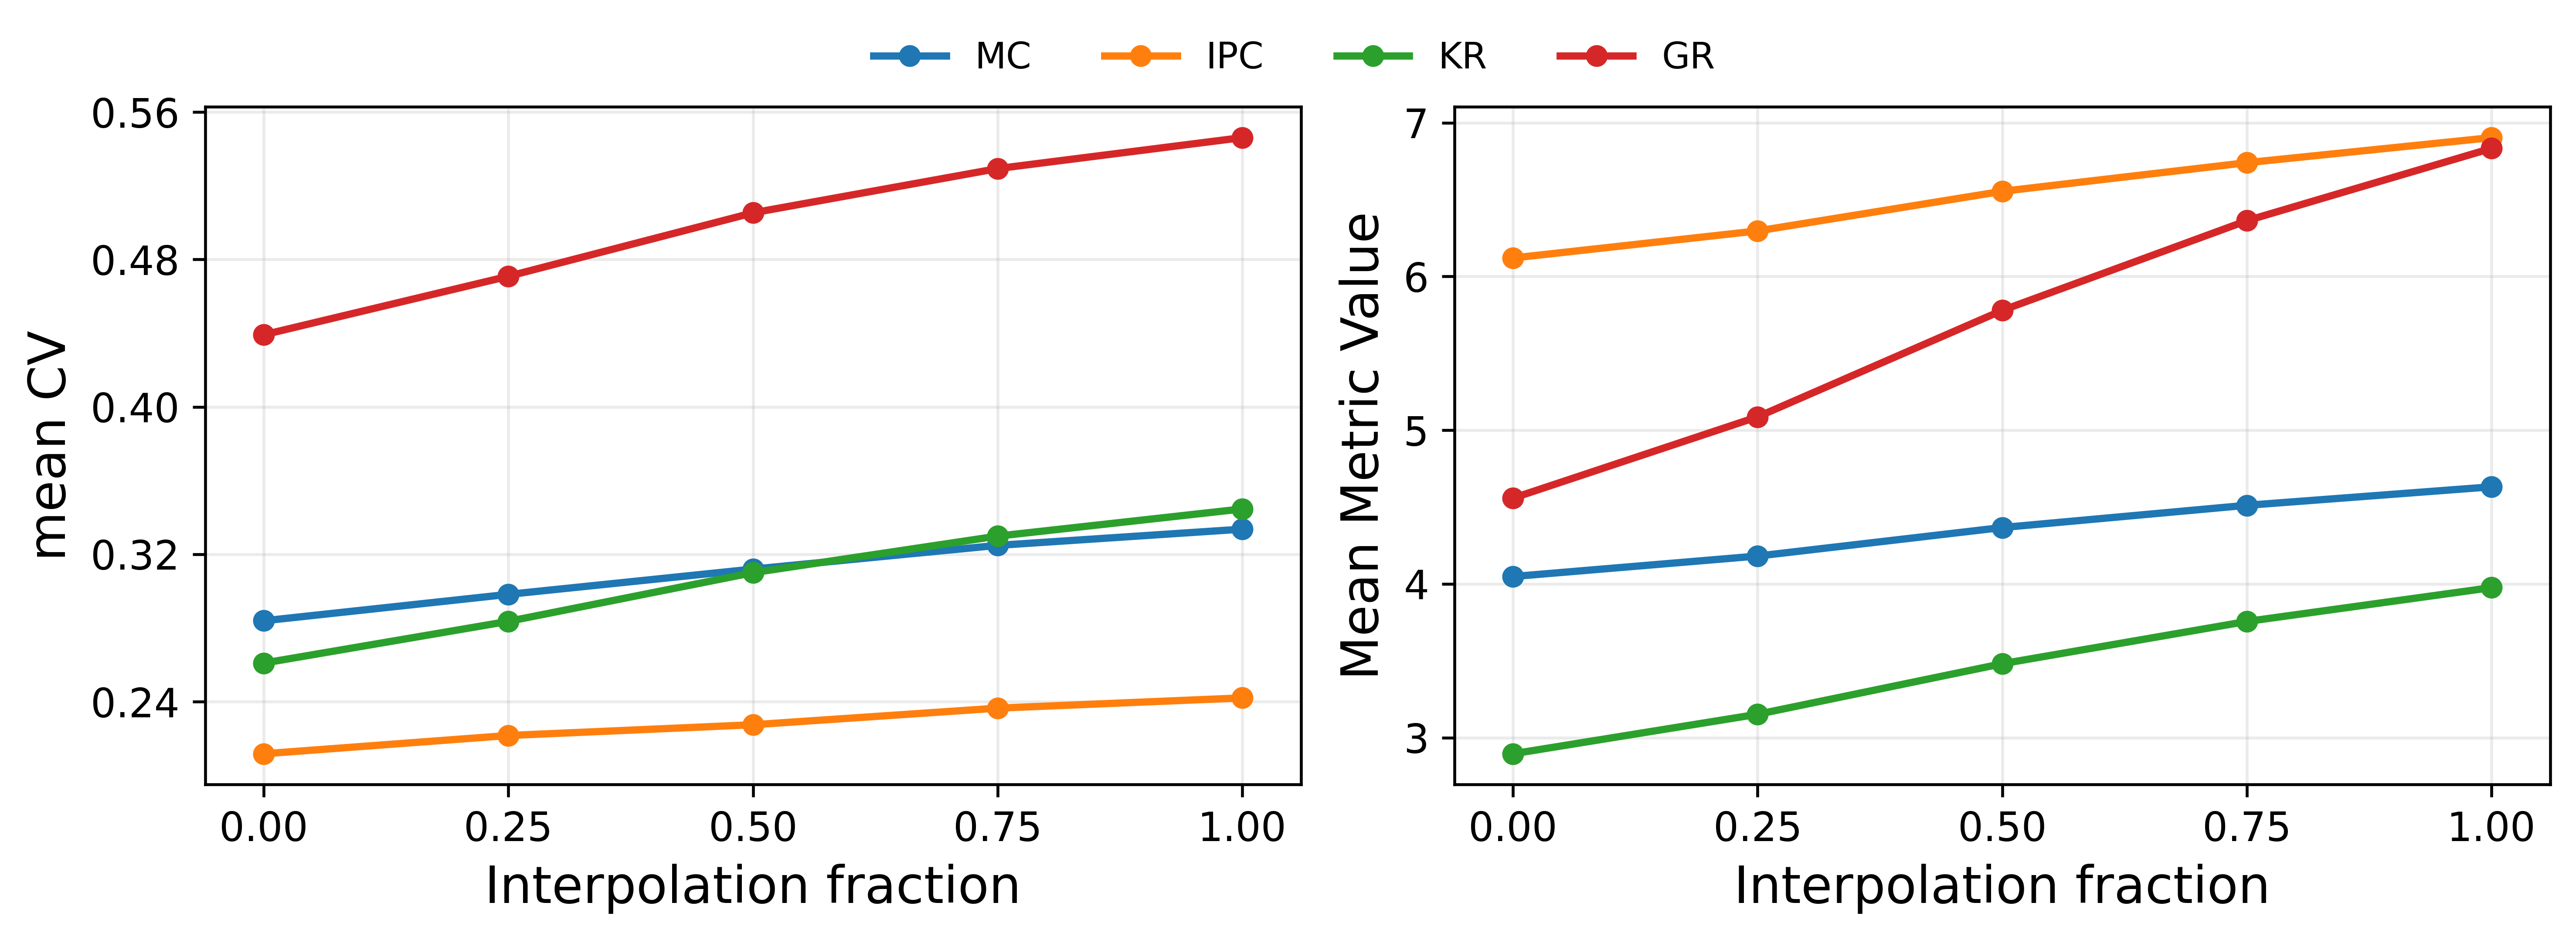
\includegraphics[width=\linewidth]{figs/interpolation/bin_to_cel_shuf.png}
    \caption{Sign-preserving interpolation from signed unit magnitudes to shuffled empirical \textit{C.\ elegans} magnitudes. The endpoint uses a random permutation of the empirical magnitudes across the original edge set while preserving each edge's original sign. Left: mean CV across the hyperparameter sweep. Right: mean task-agnostic metric value.}
    \label{fig:bin_to_cel_shuf_interp}
\end{figure}

\begin{figure}
    \centering
    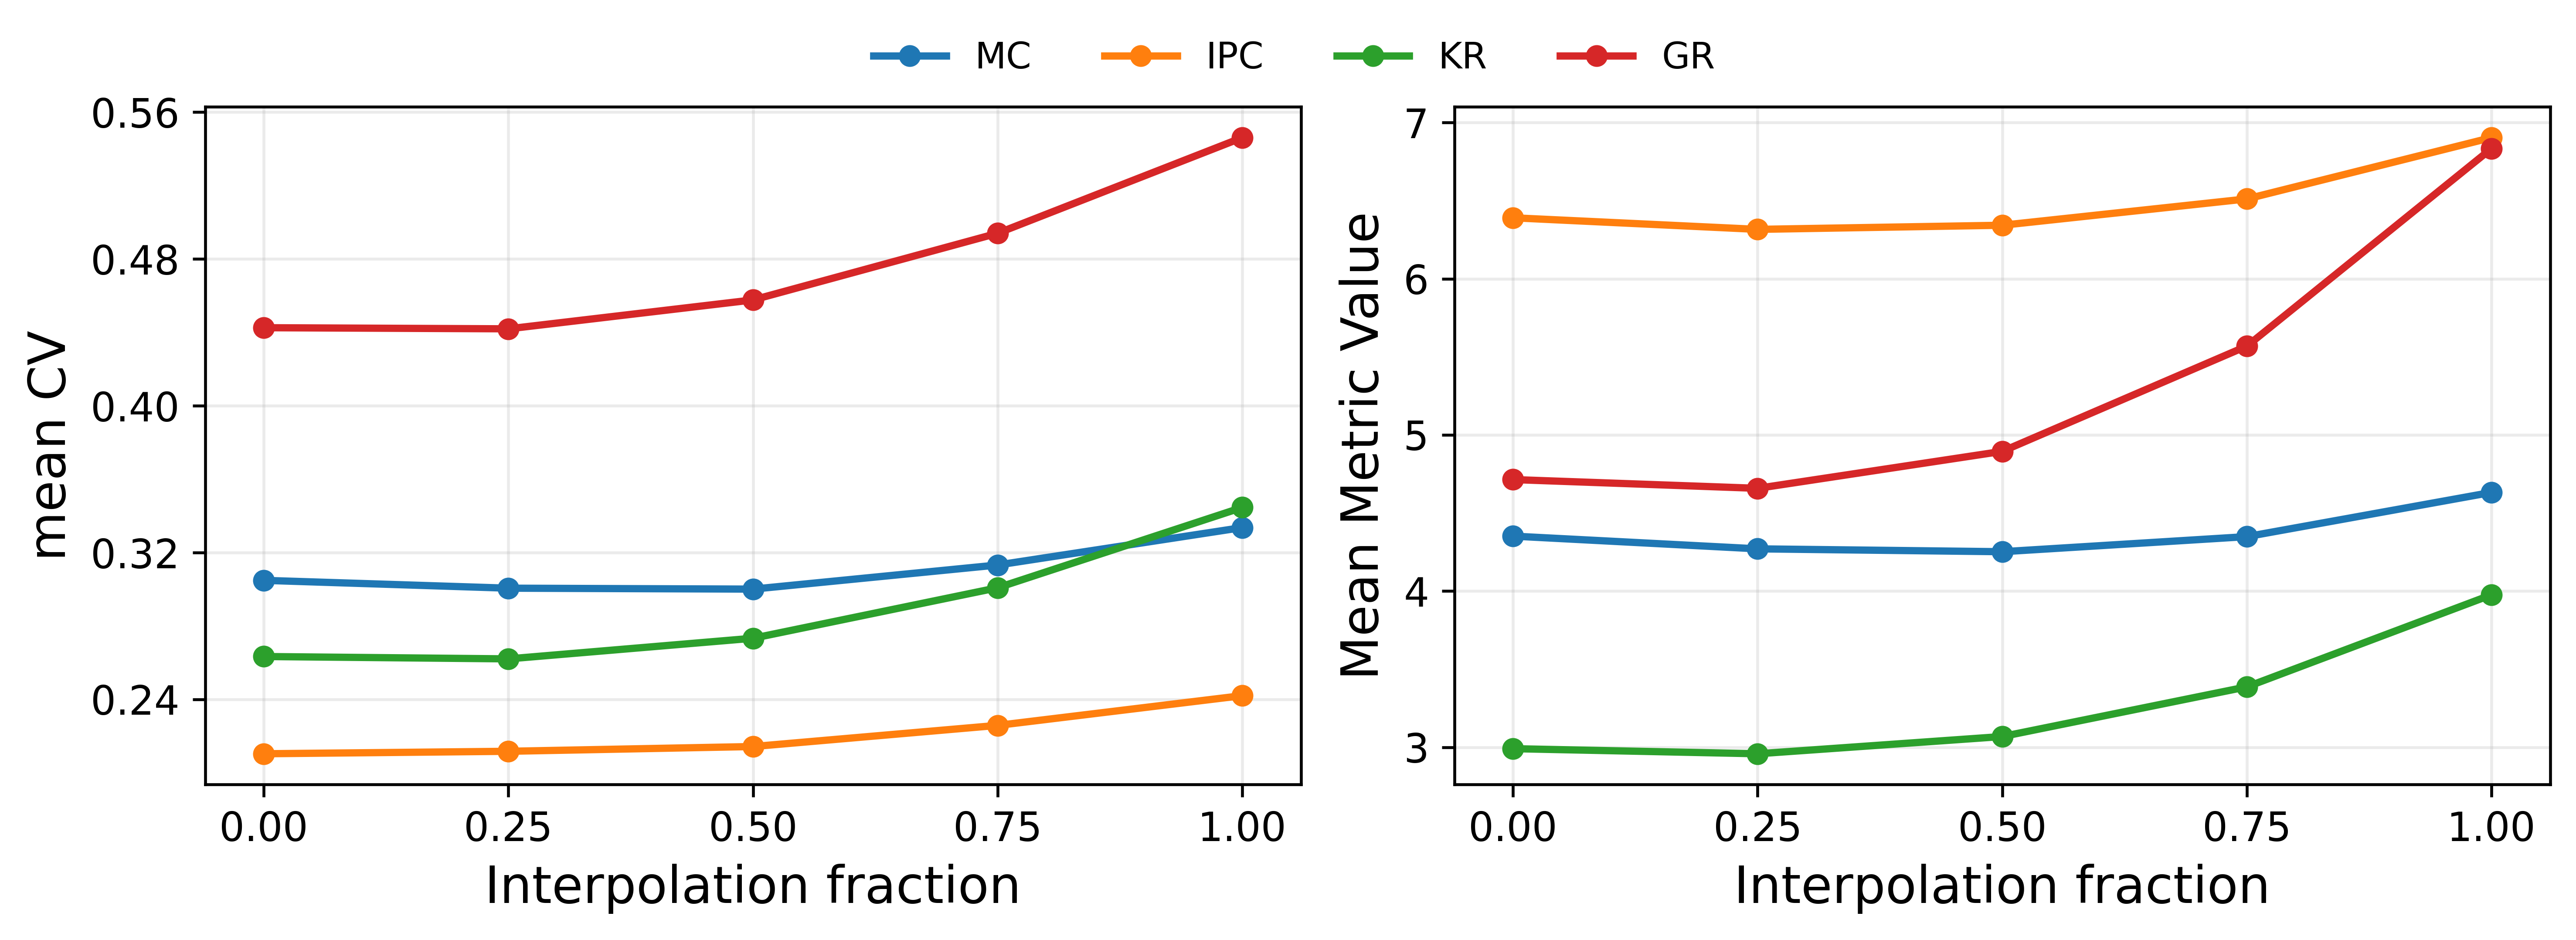
\includegraphics[width=\linewidth]{figs/interpolation/cel_to_cel_shuf.png}
    \caption{Sign-preserving interpolation from empirical \textit{C.\ elegans} magnitudes to shuffled empirical magnitudes. The endpoint redistributes empirical magnitudes across the fixed topology, but every edge retains its original sign throughout the interpolation. Left: mean CV across the hyperparameter sweep. Right: mean task-agnostic metric value.}
    \label{fig:cel_to_cel_shuf_interp}
\end{figure}

\begin{figure}
    \centering
    \includegraphics[width=\linewidth]{figs/weight_to_gaus.png}
    \caption{Effect of perturbing nonzero weight magnitudes toward a half-normal distribution while preserving connectivity and edge sign. Starting from the \textit{C.\ elegans} network, nonzero weights are transformed as $W'_{ij}=\operatorname{sign}(W_{ij})\left|W_{ij}+\Lambda Z_{ij}\right|,\qquad Z_{ij}\sim\mathcal{N}(0,1)$, where $\Lambda$ controls perturbation strength. The x-axis shows the KL divergence between the empirical distribution of $|W|$ and a fitted shifted half-normal target on a $\log_{10}$ scale; increasing $\Lambda$ decreases this divergence. Top row: mean metric value versus KL divergence. Bottom row: mean CV versus KL divergence. Colored trajectories correspond to GR (green), KR (red), IPC (orange), and MC (blue). Left and right panels show the same data from two viewing angles. The transparent planes indicate the unperturbed baseline, corresponding to $\Lambda=0$.}
    \label{fig:weights}
\end{figure}


\subsection{Neuroscience Terms Explained for Computer Scientists}
\begin{itemize}
    \item {\textbf{neuron} -- basic building block of neural circuits. In this work, neurons are represented as nodes on a graph, each with both an activation function and an internal state representing membrane potential.}
    
    \item {\textbf{synapse} -- another basic building block of neural circuits. In this work, synapses are represented by directed edges with weights connecting two neurons.} 
    \item {\textbf{excitatory neuron} -- a neuron with only positive-weight outgoing edges}
    \item {\textbf{inhibitory neuron} -- a neuron with only negative-weight outgoing edges}
    \item {\textbf{E/I balance} -- the ratio or fraction of excitatory to inhibitory synaptic signs in the modeled reservoir}
   % \item {\textbf{Dale’s law} -- principle stating that a %neuron releases the same neurotransmitter at all of its %synapses. \parencite{Svensson2019} In graph terms, neurons %adhering to this principle have all positive or negative %outgoing connections    \footnote{Dale’s law is not %universally true; many neurons are now known to exhibit %cotransmission, releasing multiple neurotransmitters and %violating the single-sign assumption.\parencite{Svensson2019} }}

    
    \item {\textbf{neurotransmitter} -- a chemical that allows neurons to communicate with each other by transmitting signals across synapses \parencite{Sheffler2023Neurotransmitters}.}
    \item {\textbf{gap junction} -- a type of synapse that connects the cytoplasm of two adjacent cells; bidirectional with the same weight for both sides. In our modeling, these are either removed or treated as two distinct positively signed edges.}
    \item {\textbf{neuromuscular junction} -- a specialized synapse where a motor neuron communicates with a muscle fiber. These directed edges point to non-neural cells and hence are not included in our graph.}
    \item {\textbf{connectome} -- a wiring diagram of a biological neural network. This typically contains all neurons and synapses, along with edge weights.}
    \item {\textbf{sensory neuron} -- a neuron that receives sensory input. During typical biological use, these can be thought of as ``inputs" to the network.} 
    \item {\textbf{motor neuron} -- a neuron that passes signals to motor cells. During typical biological use, these can be thought of as the ``outputs" of the network.}
    \item {\textbf{synaptic terminals} -- bulbous endings of a neuron's axon where neurotransmitters are transferred to other cells (neurons or muscles). We use the number of these terminals as a proxy for edge weight.}
    \item {\textbf{membrane potential} -- the difference in electrical charge between the inside and outside of a neuron, forming the basis for neural activity \parencite{Henley_2021}. For our purposes, this is the internal state of the neuron representing how much our activation function will be saturated.}
    \item {\textbf{small-worldness} -- a property commonly observed in biological networks. A graph that exhibits the small-world property has both a high clustering coefficient and a short average path length. This structure is claimed to make information spread more efficient and to make the network more robust \parencite{Bassett2007,latora2001}.}
    \item {\textbf{scale-free network}} -- a network whose degree distribution follows a power law, meaning the fraction of nodes with degree $k$ follows a power law $k^{-\alpha}$ \parencite{broido_clauset_2019}.
\end{itemize}



\subsection{Equivalence testing}
Equivalence testing using TOST (Table~\ref{tab:tost_mcipc} and Table~\ref{tab:tost_grkr}) further clarifies these relationships. We used TOST equivalence testing on the mean dispersion (CV) between each architecture and the biological connectome. The equivalence margin was set to $\Delta = |0.05(\text{median}(\text{dispersion}))|$, computed per metric across all runs. We concluded equivalence when both one-sided tests rejected the null that the mean difference lay outside $[-\Delta,+\Delta]$. Thus, small p-values indicate that the dispersion difference is statistically confined within the predefined practical tolerance. Under this criterion, only specific sign-preserving perturbations satisfied equivalence for selected metrics, while most architectures---including connection shuffles, weight shuffles, and random graph controls---did not satisfy equivalence across all metrics simultaneously. Failure to conclude equivalence (large $p$) does not imply non-equivalence; it indicates insufficient evidence that the mean difference is within $\pm\Delta$ under the chosen margin and sample size. Each comparison used 1000 observations. 


\subsection{Tables}

\begin{table}[t]
\centering
\caption{Pairwise equivalence tests (TOST) across modes within information processing capacity and memory capacity.}
\label{tab:tost_mcipc}
\begin{tabular}{llrr}
\toprule
Metric & Comparison  & TOST bound  & $p$ \\
\midrule
MC & Binary wt. vs pm1 sign-pres. + wt. shuf. & 0.0151 & 0.007238 \\
MC & Binary wt. vs pm1 sign-pres. wt. & 0.0151 & 5.5e-05 \\
MC & CE Gaussian wt. vs WS Gaussian wt. & 0.0151 & 0.02401 \\
MC & ER Gaussian wt. vs WS Gaussian wt. & 0.0151 & 5.706e-16 \\
MC & pm1 sign-pres. + wt. shuf. vs pm1 sign-pres. wt. & 0.0151 & 3.329e-16 \\
MC & pm1 sign-pres. + wt. shuf. vs Sign-pres. uniform & 0.0151 & 0.04148 \\
MC & Sign-pres. Gaussian vs Sign-pres. uniform & 0.0151 & 0.0001002 \\
MC & Sign-pres. Gaussian vs C. elegans & 0.0151 & 9.184e-12 \\
MC & Sign-pres. uniform vs C. elegans & 0.0151 & 9.91e-09 \\
\addlinespace
IPC & Binary wt. vs pm1 sign-pres. + wt. shuf. & 0.01138 & 6.972e-05 \\
IPC & Binary wt. vs pm1 sign-pres. wt. & 0.01138 & 2.129e-08 \\
IPC & Binary wt. vs C. elegans & 0.01138 & 5.563e-14 \\
IPC & ER Gaussian wt. vs WS Gaussian wt. & 0.01138 & 8.612e-08 \\
IPC & pm1 sign-pres. + wt. shuf. vs pm1 sign-pres. wt. & 0.01138 & 2.079e-11 \\
IPC & pm1 sign-pres. + wt. shuf. vs Sign-pres. uniform & 0.01138 & 1.807e-05 \\
IPC & pm1 sign-pres. + wt. shuf. vs C. elegans & 0.01138 & 1.779e-06 \\
IPC & Sign-pres. Gaussian vs Sign-pres. uniform & 0.01138 & 5.499e-06 \\
IPC & pm1 sign-pres. wt. vs Sign-pres. uniform & 0.01138 & 0.01166 \\
IPC & pm1 sign-pres. wt. vs C. elegans & 0.01138 & 1.938e-10 \\
\bottomrule
\end{tabular}
\end{table}

\begin{table}[t]
\centering
\caption{Pairwise equivalence tests (TOST) across modes within kernel rank and generalization rank.}
\label{tab:tost_grkr}
\begin{tabular}{llrr}
\toprule
Metric & Comparison  & TOST bound  & $p$ \\
\midrule
KR & ER Gaussian wt. vs WS Gaussian wt. & 0.01441 & 5.98e-05 \\
KR & pm1 sign-pres. + wt. shuf. vs pm1 sign-pres. wt. & 0.01441 & 1.116e-11 \\
KR & pm1 sign-pres. + wt. shuf. vs C. elegans & 0.01441 & 3.929e-21 \\
KR & pm1 sign-pres. wt. vs C. elegans & 0.01441 & 2.716e-20 \\
\addlinespace
GR & Binary wt. vs pm1 sign-pres. wt. & 0.02375 & 0.0459 \\
GR & CE Gaussian wt. vs ER Gaussian wt. & 0.02375 & 3.902e-06 \\
GR & CE Gaussian wt. vs WS Gaussian wt. & 0.02375 & 3.849e-08 \\
GR & ER Gaussian wt. vs WS Gaussian wt. & 0.02375 & 5.565e-65 \\
GR & pm1 sign-pres. + wt. shuf. vs pm1 sign-pres. wt. & 0.02375 & 1.613e-24 \\
GR & pm1 sign-pres. + wt. shuf. vs C. elegans & 0.02375 & 4.416e-41 \\
GR & Sign-pres. Gaussian vs Sign-pres. uniform & 0.02375 & 0.03561 \\
GR & pm1 sign-pres. wt. vs C. elegans & 0.02375 & 9.945e-45 \\
\bottomrule
\end{tabular}
\end{table}

\begin{table}[t]
\centering
\caption{Pairwise equivalence tests (TOST) across modes within information processing capacity and memory capacity for shuffling experiment 1.}
\label{tab:tost_mcipc_shuffles_1}
\begin{tabular}{llrr}
\toprule
Metric & Comparison  & TOST bound  & $p$ \\
\midrule
MC & Conn. + wt. shuf. vs Conn. shuf. & 0.01656 & 7.926e-20 \\
MC & Conn. + wt. shuf. vs Weight shuf. & 0.01656 & 1.844e-14 \\
MC & Conn. shuf. vs Weight shuf. & 0.01656 & 1.615e-15 \\
\addlinespace
IPC & Conn. + wt. shuf. vs Conn. shuf. & 0.01213 & 6.19e-07 \\
IPC & Conn. + wt. shuf. vs Weight shuf. & 0.01213 & 4.58e-09 \\
IPC & Conn. shuf. vs Weight shuf. & 0.01213 & 2.501e-12 \\
\bottomrule
\end{tabular}
\end{table}

\begin{table}[t]
\centering
\caption{Pairwise equivalence tests (TOST) across modes within kernel rank and generalization rank for shuffling experiment 1.}
\label{tab:tost_grkr_shuffles_1}
\begin{tabular}{llrr}
\toprule
Metric & Comparison  & TOST bound  & $p$ \\
\midrule
KR & Conn. + wt. shuf. vs Conn. shuf. & 0.01722 & 4.406e-30 \\
KR & Conn. + wt. shuf. vs Weight shuf. & 0.01722 & 2.781e-27 \\
KR & Conn. shuf. vs Weight shuf. & 0.01722 & 8.019e-21 \\
\addlinespace
GR & Conn. + wt. shuf. vs Conn. shuf. & 0.02759 & 4.394e-70 \\
GR & Conn. + wt. shuf. vs Weight shuf. & 0.02759 & 7.459e-46 \\
GR & Conn. shuf. vs Weight shuf. & 0.02759 & 4.201e-41 \\
\bottomrule
\end{tabular}
\end{table}

\begin{table}[t]
\centering
\caption{Pairwise equivalence tests (TOST) across modes within information processing capacity and memory capacity for shuffling experiment 2.}
\label{tab:tost_mcipc_shuffles_2}
\begin{tabular}{llrr}
\toprule
Metric & Comparison  & TOST bound  & $p$ \\
\midrule
MC & pm1 sign-pres. + shuf. vs pm1 + conn. shuf. & 0.01368 & 7.998e-12 \\
MC & pm1 sign-pres. + shuf. vs pm1 sign-pres. + wt. shuf. & 0.01368 & 0.04546 \\
MC & pm1 + conn. shuf. vs pm1 sign-pres. + wt. shuf. & 0.01368 & 7.225e-05 \\
MC & pm1 sign-pres. + wt. shuf. vs pm1 sign-pres. wt. & 0.01368 & 2.114e-05 \\
\addlinespace
IPC & pm1 sign-pres. + shuf. vs pm1 + conn. shuf. & 0.0106 & 8.308e-10 \\
IPC & pm1 sign-pres. + shuf. vs pm1 sign-pres. + wt. shuf. & 0.0106 & 2.293e-11 \\
IPC & pm1 sign-pres. + shuf. vs pm1 sign-pres. wt. & 0.0106 & 7.678e-11 \\
IPC & pm1 + conn. shuf. vs pm1 sign-pres. + wt. shuf. & 0.0106 & 1.491e-07 \\
IPC & pm1 + conn. shuf. vs pm1 sign-pres. wt. & 0.0106 & 3.382e-07 \\
IPC & pm1 sign-pres. + wt. shuf. vs pm1 sign-pres. wt. & 0.0106 & 7.407e-15 \\
\bottomrule
\end{tabular}
\end{table}

\begin{table}[t]
\centering
\caption{Pairwise equivalence tests (TOST) across modes within kernel rank and generalization rank for shuffling experiment 2.}
\label{tab:tost_grkr_shuffles_2}
\begin{tabular}{llrr}
\toprule
Metric & Comparison  & TOST bound  & $p$ \\
\midrule
KR & pm1 sign-pres. + shuf. vs pm1 + conn. shuf. & 0.01317 & 4.991e-12 \\
KR & pm1 sign-pres. + shuf. vs pm1 sign-pres. + wt. shuf. & 0.01317 & 6.44e-08 \\
KR & pm1 sign-pres. + shuf. vs pm1 sign-pres. wt. & 0.01317 & 2.063e-20 \\
KR & pm1 + conn. shuf. vs pm1 sign-pres. + wt. shuf. & 0.01317 & 4.512e-16 \\
KR & pm1 + conn. shuf. vs pm1 sign-pres. wt. & 0.01317 & 1.584e-13 \\
KR & pm1 sign-pres. + wt. shuf. vs pm1 sign-pres. wt. & 0.01317 & 3.403e-09 \\
\addlinespace
GR & pm1 sign-pres. + shuf. vs pm1 + conn. shuf. & 0.02224 & 3.981e-30 \\
GR & pm1 sign-pres. + shuf. vs pm1 sign-pres. + wt. shuf. & 0.02224 & 1.419e-47 \\
GR & pm1 sign-pres. + shuf. vs pm1 sign-pres. wt. & 0.02224 & 9.588e-23 \\
GR & pm1 + conn. shuf. vs pm1 sign-pres. + wt. shuf. & 0.02224 & 7.492e-30 \\
GR & pm1 + conn. shuf. vs pm1 sign-pres. wt. & 0.02224 & 9.344e-10 \\
GR & pm1 sign-pres. + wt. shuf. vs pm1 sign-pres. wt. & 0.02224 & 1.875e-20 \\
\bottomrule
\end{tabular}
\end{table}


\begin{table}[t]
\centering
\caption{Pairwise equivalence tests (TOST) across modes within kernel rank and generalization rank for shuffling experiment 3.}
\label{tab:tost_grkr_shuffles_3}
\begin{tabular}{llrr}
\toprule
Metric & Comparison  & TOST bound  & $p$ \\
\midrule
IPC & Binary wt. vs Binary wt. + shuf. & 0.01039 & 2.887e-08 \\
\addlinespace
KR & Binary wt. vs Binary wt. + shuf. & 0.01215 & 0.002745 \\
\addlinespace
GR & Binary wt. vs Binary wt. + shuf. & 0.02068 & 5.831e-35 \\
\bottomrule
\end{tabular}
\end{table}

\begin{table}[t]
\centering
\caption{Changes in mean CV across Gaussian noise magnitudes. Baseline column lists the reference value for each metric; other entries show absolute change followed by percent change. Relative to baseline mode weight\_test0.0. Sign is not preserved in this version of the experiment.}
\label{tab:no_sign_pres_gaus_weights}
\begin{tabular}{lcccc}
\toprule
Metric & Baseline & $\Lambda=1$ & $\Lambda=5$ & $\Lambda=10$ \\
\midrule
MC & 0.3548 & +0.00808 (+2.28\%) & +0.0851 (+24\%) & +0.162 (+45.6\%)  \\
IPC & 0.2718 & +0.00868 (+3.19\%) & +0.0891 (+32.8\%) & +0.151 (+55.4\%) \\
KR & 0.2634 & +0.00505 (+1.92\%) & +0.125 (+47.6\%) & +0.335 (+127\%) \\
GR & 0.4426 & +0.00829 (+1.87\%) & +0.162 (+36.5\%) & +0.311 (+70.3\%) \\
\bottomrule
\end{tabular}
\end{table}
\begin{table}[t]
\centering
\caption{Changes in mean metric value across Gaussian noise magnitudes. Baseline column lists the reference value for each metric; other entries show absolute change followed by percent change. Relative to baseline mode weight\_test0.0. Sign is not preserved in this version of the experiment.}
\label{tab:no_sign_pres_gaus_metric_mean}
\begin{tabular}{lcccc}
\toprule
Metric & Baseline & $\Lambda=1$ & $\Lambda=5$ & $\Lambda=10$ \\
\midrule
MC & 4.161 & +0.00525 (+0.126\%) & +0.715 (+17.2\%) & +3.13 (+75.3\%) \\
IPC & 5.863 & +0.0241 (+0.411\%) & +0.999 (+17\%) & +4.31 (+73.4\%)  \\
KR & 2.99 & +0.0545 (+1.82\%) & +1.6 (+53.4\%) & +7.51 (+251\%)  \\
GR & 4.712 & +0.12 (+2.55\%) & +3.54 (+75\%) & +16.4 (+348\%) \\
\bottomrule
\end{tabular}
\end{table}

\begin{table}[t]
\centering
\caption{Changes in mean CV across Gaussian noise magnitudes. Baseline column lists the reference value for each metric; other entries show absolute change followed by percent change. Relative to baseline mode weight\_test0.0. Sign is preserved in this version of the experiment.}
\label{tab:sign_pres_gaus_weights}
\begin{tabular}{lcccc}
\toprule
Metric & Baseline & $\Lambda=1$ & $\Lambda=5$ & $\Lambda=10$ \\
\midrule
MC & 0.3623 & +0.00232 (+0.641\%) & +0.0133 (+3.67\%) & +0.0156 (+4.32\%) \\
IPC & 0.2781 & +0.00298 (+1.07\%) & +0.0178 (+6.38\%) & +0.0244 (+8.76\%) \\
KR & 0.2634 & +0.00294 (+1.12\%) & +0.0211 (+8.01\%) & +0.0306 (+11.6\%) \\
GR & 0.4426 & +0.00508 (+1.15\%) & +0.0319 (+7.2\%) & +0.0444 (+10\%) \\
\bottomrule
\end{tabular}
\end{table}
\begin{table}[t]
\centering
\caption{Changes in mean metric value across Gaussian noise magnitudes. Baseline column lists the reference value for each metric; other entries show absolute change followed by percent change. Relative to baseline mode weight\_test0.0. Sign is preserved in this version of the experiment.}
\label{tab:sign_pres_gaus_metric_mean}
\begin{tabular}{lcccc}
\toprule
Metric & Baseline & $\Lambda=1$ & $\Lambda=5$ & $\Lambda=10$ \\
\midrule
MC & 4.096 & -0.00846 (-0.206\%) & -0.094 (-2.3\%) & -0.102 (-2.48\%) \\
IPC & 5.733 & +0.00524 (+0.0914\%) & -0.0257 (-0.448\%) & -0.0286 (-0.499\%) \\
KR & 2.99 & +0.0314 (+1.05\%) & +0.193 (+6.45\%) & +0.289 (+9.67\%) \\
GR & 4.712 & +0.0731 (+1.55\%) & +0.447 (+9.49\%) & +0.655 (+13.9\%) \\
\bottomrule
\end{tabular}
\end{table}

\begin{table}[t]
\centering
\caption{Changes in mean CV during sign-preserving interpolation from signed unit magnitudes to empirical \textit{C.\ elegans} magnitudes. Baseline column lists the value at \(f=0\); other entries show absolute change followed by percent change.}
\label{tab:bin_to_cel_interp_cv}
\resizebox{\textwidth}{!}{\begin{tabular}{lccccc}
\toprule
Metric & Baseline & $f=0.25$ & $f=0.5$ & $f=0.75$ & $f=1$ \\
\midrule
MC & 0.2839 & +0.00492 (+1.73\%) & +0.0134 (+4.72\%) & +0.0173 (+6.1\%) & +0.021 (+7.39\%) \\
IPC & 0.2117 & -0.00641 (-3.03\%) & -0.00466 (-2.2\%) & -0.00324 (-1.53\%) & -0.00134 (-0.635\%) \\
KR & 0.2609 & -0.00808 (-3.1\%) & -0.00403 (-1.54\%) & -0.000338 (-0.129\%) & +0.00242 (+0.929\%) \\
GR & 0.4391 & -0.00993 (-2.26\%) & -0.00448 (-1.02\%) & +0.000223 (+0.0509\%) & +0.0034 (+0.775\%) \\
\bottomrule
\end{tabular}
}
\end{table}

\begin{table}[t]
\centering
\caption{Changes in mean metric value during sign-preserving interpolation from signed unit magnitudes to empirical \textit{C.\ elegans} magnitudes. Baseline column lists the value at \(f=0\); other entries show absolute change followed by percent change.}
\label{tab:bin_to_cel_interp_perf}
\resizebox{\textwidth}{!}{\begin{tabular}{lccccc}
\toprule
Metric & Baseline & $f=0.25$ & $f=0.5$ & $f=0.75$ & $f=1$ \\
\midrule
MC & 4.048 & +0.0868 (+2.14\%) & +0.193 (+4.76\%) & +0.264 (+6.51\%) & +0.304 (+7.5\%) \\
IPC & 6.121 & +0.048 (+0.784\%) & +0.154 (+2.51\%) & +0.226 (+3.69\%) & +0.27 (+4.4\%) \\
KR & 2.895 & -0.0557 (-1.92\%) & +0.0046 (+0.159\%) & +0.0564 (+1.95\%) & +0.0957 (+3.31\%) \\
GR & 4.558 & -0.125 (-2.75\%) & -0.0156 (-0.342\%) & +0.0825 (+1.81\%) & +0.156 (+3.42\%) \\
\bottomrule
\end{tabular}
}
\end{table}

\begin{table}[t]
\centering
\caption{Changes in mean CV during sign-preserving interpolation from signed unit magnitudes to shuffled empirical \textit{C.\ elegans} magnitudes. Baseline column lists the value at \(f=0\); other entries show absolute change followed by percent change.}
\label{tab:bin_to_cel_shuf_interp_cv}
\resizebox{\textwidth}{!}{\begin{tabular}{lccccc}
\toprule
Metric & Baseline & $f=0.25$ & $f=0.5$ & $f=0.75$ & $f=1$ \\
\midrule
MC & 0.2839 & +0.0143 (+5.05\%) & +0.028 (+9.88\%) & +0.0409 (+14.4\%) & +0.0497 (+17.5\%) \\
IPC & 0.2117 & +0.00991 (+4.68\%) & +0.0157 (+7.44\%) & +0.0247 (+11.7\%) & +0.0303 (+14.3\%) \\
KR & 0.2609 & +0.0226 (+8.68\%) & +0.0491 (+18.8\%) & +0.0689 (+26.4\%) & +0.0836 (+32.1\%) \\
GR & 0.4391 & +0.0317 (+7.23\%) & +0.0662 (+15.1\%) & +0.0902 (+20.5\%) & +0.107 (+24.4\%) \\
\bottomrule
\end{tabular}
}
\end{table}

\begin{table}[t]
\centering
\caption{Changes in mean metric value during sign-preserving interpolation from signed unit magnitudes to shuffled empirical \textit{C.\ elegans} magnitudes. Baseline column lists the value at \(f=0\); other entries show absolute change followed by percent change.}
\label{tab:bin_to_cel_shuf_interp_perf}
\resizebox{\textwidth}{!}{\begin{tabular}{lccccc}
\toprule
Metric & Baseline & $f=0.25$ & $f=0.5$ & $f=0.75$ & $f=1$ \\
\midrule
MC & 4.048 & +0.133 (+3.29\%) & +0.319 (+7.87\%) & +0.463 (+11.4\%) & +0.583 (+14.4\%) \\
IPC & 6.121 & +0.176 (+2.88\%) & +0.434 (+7.09\%) & +0.62 (+10.1\%) & +0.783 (+12.8\%) \\
KR & 2.895 & +0.257 (+8.88\%) & +0.586 (+20.2\%) & +0.861 (+29.7\%) & +1.08 (+37.3\%) \\
GR & 4.558 & +0.529 (+11.6\%) & +1.22 (+26.8\%) & +1.81 (+39.6\%) & +2.28 (+49.9\%) \\
\bottomrule
\end{tabular}
}
\end{table}

\begin{table}[t]
\centering
\caption{Changes in mean CV during sign-preserving interpolation from empirical \textit{C.\ elegans} magnitudes to shuffled empirical magnitudes. Baseline column lists the value at \(f=0\); other entries show absolute change followed by percent change.}
\label{tab:cel_to_cel_shuf_interp_cv}
\resizebox{\textwidth}{!}{\begin{tabular}{lccccc}
\toprule
Metric & Baseline & $f=0.25$ & $f=0.5$ & $f=0.75$ & $f=1$ \\
\midrule
MC & 0.3049 & -0.00427 (-1.4\%) & -0.00478 (-1.57\%) & +0.00836 (+2.74\%) & +0.0287 (+9.43\%) \\
IPC & 0.2104 & +0.00135 (+0.642\%) & +0.00394 (+1.87\%) & +0.0155 (+7.35\%) & +0.0317 (+15\%) \\
KR & 0.2634 & -0.00128 (-0.486\%) & +0.00995 (+3.78\%) & +0.0375 (+14.2\%) & +0.0812 (+30.8\%) \\
GR & 0.4425 & -0.000606 (-0.137\%) & +0.0151 (+3.42\%) & +0.0515 (+11.6\%) & +0.104 (+23.4\%) \\
\bottomrule
\end{tabular}
}
\end{table}

\begin{table}[t]
\centering
\caption{Changes in mean metric value during sign-preserving interpolation from empirical \textit{C.\ elegans} magnitudes to shuffled empirical magnitudes. Baseline column lists the value at \(f=0\); other entries show absolute change followed by percent change.}
\label{tab:cel_to_cel_shuf_interp_perf}
\resizebox{\textwidth}{!}{\begin{tabular}{lccccc}
\toprule
Metric & Baseline & $f=0.25$ & $f=0.5$ & $f=0.75$ & $f=1$ \\
\midrule
MC & 4.352 & -0.0815 (-1.87\%) & -0.0999 (-2.3\%) & -0.00326 (-0.075\%) & +0.28 (+6.43\%) \\
IPC & 6.39 & -0.0742 (-1.16\%) & -0.0477 (-0.747\%) & +0.121 (+1.89\%) & +0.513 (+8.03\%) \\
KR & 2.991 & -0.0327 (-1.09\%) & +0.0777 (+2.6\%) & +0.396 (+13.2\%) & +0.985 (+32.9\%) \\
GR & 4.714 & -0.0561 (-1.19\%) & +0.181 (+3.83\%) & +0.855 (+18.1\%) & +2.12 (+45\%) \\
\bottomrule
\end{tabular}
}
\end{table}
\bibliographystyle{style_neural_networks/cas-model2-names}
\bibliography{bibliography}

% Finally, an index would go here... but it is also optional.
\end{document}
